% [-] MonasPlusを消す

\documentclass[a5paper,twoside,fleqn,draft]{jsbook}
% \usepackage{eulervm}
\usepackage{amsmath,amssymb,ascmac,stmaryrd,bm,graphicx,latexsym,mathtools,multirow,okuverb}
\usepackage[dvipsnames]{xcolor}
\usepackage{hskl,old-hskl}
\makeindex

\title{関数型プログラミングと代数構造}
\author{金谷一朗}

\begin{document}
% \setlength{\baselineskip}{17pt}
\maketitle
\tableofcontents

\begin{table*}[p]
\caption{凡例 (1)}
\begin{center}
\begin{tabular}{||c|c|c||}
\hline
種類&字体・表記法&例\\
\hline\hline
定数&イタリック大文字(1文字)&$\hConstant{A},\hConstant{B},\hConstant{C}$\\
有名な定数&ローマン大文字&$\hTrue,\hFalse$\\
単位元(数学)&ローマンに斜線&$\hZero$\\
\hline
変数&イタリック(1文字)&$\hVar{u},\hVar{v},\hVar{w},\hVar{x},\hVar{y},\hVar{z}$\\
リスト変数&sをつける&$\hListVar{x}$\\ %%% !!!
Maybe変数&?をつける&$\hMaybeDecor{\hVar{x}}$\\ %%% !!!
Ether変数&!をつける&$\hEitherDecor{\hVar{x}}$\\ %%% !!!
一般のコンテナ変数&星印をつける&$\hAnyContextVar{x}$\\
有名な変数&ローマン&$\hSpecialVar{first},\hSpecialVar{rest}$\\
\hline
関数&イタリック(1文字)&$\hFunc{f},\hFunc{g},\hFunc{h}$\\
% 一般のコンテナ関数&&$\hAnyContextDecor{\hFunc{f}}$\\ %%% !!!
有名な関数&ローマン&$\hId,\hSin,\hCos$\\
関手&フラクチュール&$\hCatId$\\
\hline
アクション&ギリシア文字(1文字)&$\hAction{\alpha},\hAction{\omega}$\\
有名なアクション&スラント&$\hMain,\hReturn$\\ %%% !!!
\hline
型&ボールド(1文字)&$\hTypeName{a},\hTypeName{b},\hTypeName{c}$\\
有名な型&ボールド大文字&$\hBool,\hInt$\\
型クラス&スモールキャピタル&$\hEq,\hOrd$\\
型コンストラクタ&ボールドイタリック&$\hTypeConstructor{m},\hTypeConstructor{n}$\\
有名な型コンストラクタ&ボールド大文字&$\hList,\hMaybe$\\
多相型&型コンストラクタ名と型名&$\hTypeConstruct{\hTypeConstructor{m}}{\hTypeName{a}}$\\
有名な多相型&同上&$\hMaybeConstruct{\hTypeName{a}}$\\
有名な多相型&特別な括弧で包む&$[\hTypeName{a}]$\\
集合(数学)&ブラックボード大文字&$\hSet{B},\hSet{Z},\hSet{R}$\\
\hline
\end{tabular}
\end{center}
\end{table*}

\begin{table*}[p]
\caption{凡例 (2)}
\begin{center}
\begin{tabular}{||c|c|c||}
\hline
種類&字体・表記法&例\\
\hline\hline
値コンストラクタ&名前付き括弧で包む&$\hLeftWith{\hVar{x}},\hRightWith{\hVar{x}}$\\
有名な値コンストラクタ&特別な括弧で包む&$\hListWith{\hVar{x}}$\\
\hline
キーワード&サンセリフ&$\hIf,\hOtherwise$\\
do記法中のキーワード&タイプライタ&$\hDoLet$\\
% リストの構造&サンセリフ,大文字&$\hTypeName{a}thFirst$, $\hTypeName{a}thRest$\\
\hline
リスト&ブラケットで包む&$\hListWith{\hVar{x}},\hListWith{\hVar{y}}$\\
タプル&丸括弧で包む&$\hPairWith{\hVar{x}}{\hVar{y}}$\\
\hline
集合(数学)&ブレースで包む&$\{\hVar{x},\hVar{y}\}$\\
% アンボックス化タプル&丸括弧とシャープ記号で包む&$\mTupleUnboxedWith{x,\hVar{y},\hVar{z}}$\\
\hline
\end{tabular}
\end{center}
\end{table*}

\begin{table*}[p]
\caption{記号一覧 (1)}
\begin{center}
\begin{tabular}{||c|c|c||}
\hline
記号&意味&\haskell 記号\\
\hline\hline
$\hLambda\hVar{x}\hLambdaArrow\hVar{x}$&ラムダ式&\verb|\x -> x|\\
$\hAnonParam$&無名パラメタ&\\
$(\hAnonParam+\hAnonParam)\,\hVar{x}\,\hVar{y}$&関数化&\code{(+) x y}\\
$\hVar{x}\hInfixWith{\hFunc{f}}\hVar{y}$&中置演算子化&\code{x `f` y}\\
\hline
$\hIsTypeOf$&型集合の元&\code{::}\\
$\hIsElementOf$&値集合の元&\code{<-}\\
$\hFunctionArrow$&射&\code{->}\\
\hline
$\hForall{\hTypeName{s}}$&全称量化子&\code{forall s.}\\
\hline
$\hFromIntegral$&型変換演算子&\code{fromIntegral}\\ %%% !!!
$\hToEnum$&同上&\code{toEnum}\\
\hline
$\hFold$&左畳み込み&\code{foldl}\\
$\hFoldRight$&右畳み込み&\code{foldr}\\
\hline
$\hCons$&cons演算子&\code{:}\\
$\hAppend$&結合演算子&\code{++}\\
\hline
$\hUnit$&ユニット&\code{()}\\
$\hEmptyList$&空リスト&\code{[]}\\
$\hNothing$&ナッシング&\code{Nothing}\\
\hline
$\hPureNothing$&空&\\
\hline
$\hListWith{\hVar{x}}$&リスト値コンストラクタ&\code{[x]}\\
$\hJustWith{\hVar{x}}$&Maybe値コンストラクタ&\code{Just x}\\
$\hLeftWith{\hVar{x}},\hRightWith{\hVar{x}}$&Either値コンストラクタ&\code{Left x}, \code{Right x}\\
\hline

\end{tabular}
\end{center}
\end{table*}

\begin{table*}[p]
\caption{記号一覧 (2)}
\begin{center}
\begin{tabular}{||c|c|c||}
\hline
記号&意味&\haskell 記号\\
\hline\hline
$\hMap$&リストのマップ&\code{`map`}\\
$\hMapM$&文脈付きリストのマップ&\code{`mapM`}\\
$\hMaybeMap$&Maybeのマップ&\code{<\$>}, \code{`fmap`}\\
$\hFunctorMap$&ファンクターのマップ&\code{<\$>}, \code{`fmap`}\\
$\hApplicativeMap$&アプリカティブマップ&\code{<*>}, \code{`ap`}\\
$\hMonadicBind$&モナドのバインド&\code{=<<}\\
\hline
$\hRightMonadicBind$&右バインド演算子&\code{>>=}\\
$\hRightMonadicBindIgnore$&右バインド演算子(戻値無視)&\code{>>}\\
\hline
$\hApply$&関数の適用&\code{\$}\\
$\hCompose$&関数の合成&\code{.}\\
$\hMonadicCompose$&モナドの合成&\code{<=<}\\
\hline
$\hArrowArrow$&&\code{>>>}\\
$\hArrowAnd$&&\code{\&\&\&}\\
$\hArrowOr$&&\code{|||}\\
% $\mLLL$&カテゴリ関数合成&\code{<<<}\\
\hline
\end{tabular}
\end{center}
\end{table*}

\part{関数型プログラミング*}

\chapter{はじめに*}
\label{ch:introduction}

\begin{leader}
本書はプログラミング言語\haskell の入門書である.それと同時に,本書はプログラミング言語を用いた代数構造の入門書でもある.プログラミングと代数構造の間には密接な関係があるが,特に関数型プログラミングを実践する時にはその関係を意識する必要が出てくる.本書はその両者を同時に解説することを試みる.
\end{leader}

\section{\haskell という森}

これからのプログラマにとって\haskell を無視することはできない.\haskell の「欠点をあげつらうことも,攻撃することもできるが,無視することだけはできない」のだ.それは\haskell がプログラミングの本質に深く関わっているからである.

\haskell というプログラミング言語を知ろうとすると,従来のプログラミング言語の知識が邪魔をする.モダンで,人気があって,\haskell から影響を受けた言語,例えば\ruby や\swift の知識さえ,\haskell を学ぶ障害になり得る.ではどのようにして\haskell の深みに到達すればいいのだろうか.

その答えは,一見遠回りに見えるが,一度抽象数学の高みに登ることである.

と言っても,あわてる必要はない.

近代的なプログラミング言語を知っていれば,すでにある程度抽象数学に足を踏み入れているからである.そこで,本書では近代的なプログラマを対象に,プログラミング言語を登山口に抽象数学の山を登り,その高みから\haskell という森を見下ろすことにする.

%% REWRITE %%

さて,登山口にどのプログラミング言語を選ぶのが適当であろうか.TIOBE Index 2023年2月版によると「ビッグ5」として \python, \clang, \cxx, \java, \csharp\ が挙げられている.\footnote{\textURL{https://www.tiobe.com/tiobe-index/}}順位の変動はあるが,他の調査でもビッグ5は過去何年も変動していないので,当座は妥当な統計であろう.このうち\clang は「多くのプログラマが読める」以外にメリットが無く,その唯一のメリットさえ最近は怪しくなっているため,登山口候補から外す.残るは\java, \cxx, \csharp\ グループと\python ということになるが,シンプルであり,かつ\haskell と対極にある言語である\python を登山口に選ぶことにした.

本書では\python コードはこのように登場する.
\begin{pythoncode}
\begin{verbatim}
print("Hello, world.")
\end{verbatim}
\end{pythoncode}
本書に示すコードは擬似コードではなく,すべて実行可能な本物のコードである.

ところで,一部の章でどうしても型に触れないといけない部分がある.\python は動的型付け言語であり,型の説明には不適切であるため,この部分だけ理解の助けとして\cxxseventeen によるコードを例示した.この部分はコードを読まなくても先に進める.

\separator

ところで,プログラムのソースコードは現代でもASCII文字セットの範囲で書くことが標準的である.Unicodeを利用したり,まして文字にカラーを指定したり,書体や装飾を指定することは一般的ではない.例えば変数 \code{a} のことを \textbf{a} と書いたり \underline{a} と書いたり $\Hat a$ と書いたりして区別することはない.

\haskell プログラマもまた,多くの異なる概念を同じ貧弱な文字セットで表現しなければならない.これは,初めて\haskell コードを読むときに大きな問題になり得る.例えば\haskell では \code{[a]} という表記をよく扱う.この \code{[a]} は \code{a} という変数1要素からなるリストのこともあるし, \code{a} 型という仮の型から作ったリスト型の場合もあるが,字面からでは判断できない.もし変数はイタリック体,型はボールド体と決まっていれば,それぞれ $\hListWith{\hVar{a}}$ および $\hListConstruct{\hTypeName{a}}$ と区別出来たところである.

本書は,異なる性質のものには異なる書体を割り当てるようにしている.ただし,どの表現もいつでも\haskell に翻訳できるように配慮している.実際,本書執筆の最大の困難点は,数学的に妥当で,かつ\haskell の記法とも矛盾しない記法を見つけることであった.

\section{関数型プログラミング}

プログラマはなぜ\haskell を習得しなければならないのだろう.それは\haskell と\keyword{関数型プログラミング}の間に密接な関係があるからである.

関数型プログラミングとはプログラミングにおける一種のスローガンのようなもので,どの言語を用いたから関数型でどの言語を用いたから関数型ではない,というものではない.しかし,関数型プログラミングを強くサポートする言語と,そうでない言語とがある.ここら辺の事情はオブジェクト指向プログラミングとプログラミング言語の関係と似ている.\haskell は関数型プログラミングを強くサポートし,\python はほとんどサポートしない.

関数型プログラミングの特徴を一言で言えば,プログラム中の\keyword{破壊的代入}を禁止することである.変数 $\hVar{x}$ に $\hConstant{1}$ という数値が一度代入されたら,変数 $\hVar{x}$ の値をプログラム中に書き換える,すなわち破壊的代入をすることはできない.この結果,変数の値はプログラムのどこでも,どの時点で読み出しても同じであることが保証される.これを変数の\keyword{参照透過性}と呼ぶ.

プログラム全体に参照透過性があると,そのプログラムはブロックに分割しやすく,各々のブロックは再利用しやすい.またプログラムのどの断片から読み始めても,全体の構造を見失いにくい.これが関数型プログラミングとそれを強くサポートする\haskell を習得する理由である.

参照透過性がもたらすもう一つのボーナスは変数の\keyword{遅延評価}である.変数はいつ評価しても値が変わらないのだから,コンパイラは変数をできるだけ遅く評価してよい.この遅延評価によって,\haskell コンパイラは他の言語に見られない\keyword{無限リスト}を扱う能力を獲得している.

\separator

ここで数学とプログラミングの関係について述べておこう.ある方程式を解くためにコンピュータによって数値シミュレーションを行うとか,非常に複雑な微分を機械的に行うとか,プログラミングによって数学をサポートすることは計算機科学の主たる分野の一つであるが,ここではもっと根源的な話をする.

数学者もプログラマも\keyword{関数}をよく使う.数学者が使う関数とは,引数がいくつかあって,その結果決まる戻り値があるようなものだ.一方でプログラマが使う関数というのは,引数と戻り値はだいたい同じとして,中身に条件分岐があったり,ループがあったり,外部変数を書き換えたり,入出力をしたりする.

どちらも同じ関数であるのに,なぜこうもイメージが違うのだろうか.

もし,我々が関数型プログラミングの原則を忠実に守り,プログラム中のいかなる破壊的代入をも禁止するとすると,両者の関数は全く同じ性格になる.逐次実行も条件分岐もループも,それどころか定数さえ,\keyword{ラムダ式}という式だけで書けるようになる.あらゆるプログラムが,最終的には単一のラムダ式で書ける.

ところが,入出力,状態変数,例外など,プログラミングに使われる多くのテクニックは関数の副作用を前提としている.参照透過性と副作用を統一的に扱うためには\keyword{モナド}という数学概念が必要である.\haskell はモナドを陽に扱うプログラミング言語である.

% 数学とプログラミングの関係

% ラムダ式は単純で,十分に数学的に定式化できるものだ.

% \section{色気のない文字セットが引き起こす問題}


% プログラマというのは口数の少ない人種なのかもしれない.

% 標準\clang が制定される前の\clang 言語のことを\clangkr と呼ぶが,\clangkr ではこんなコードが当たり前のように書かれていた.
% \begin{ckrcode}
% \begin{verbatim}
% main(argc, argv) {
%   /* do something */
%   return 0;
% }
% \end{verbatim}
% \end{ckrcode}
% 現代の標準\clang なら
% \begin{ccode}
% \begin{verbatim}
% int main(int argc, const char *const *argv) {
%   /* do something */
%   return 0;
% }
% \end{verbatim}
% \end{ccode}
% と書かれるべきところ,関数 \code{main} もその引数 \code{argc} も \code{argv} も,型が明示されていないのである.

% これは\clangkr プログラマにとって,型 \code{int} はありふれているので自明であり,ポインタは \code{int} と同一視しても問題ないと認識されていたからである.


\section{\haskell コンパイラの準備*}

本書の第I部は\haskell コンパイラ無しで読み進めることができる.とは言え,前もって\haskell コンパイラを用意しておくことは無意味とも言えない.

\TK{To be written.}

% \haskell コンパイラの中で最もよく使われているものは Glasgow's HaskellCompiler (GHC) である.本書に登場する\haskell コードもすべてGHCでテストをしている.GHCは2015年にリリースされたバージョン7.10とそれまでのバージョンとの間に大きな違いがある.本書はバージョン7.10以降を対象としているため,一部は古い書籍と互換性がない.

% GHCは公式サイト\cite{haskellplatform}からダウンロード可能であるが,GNU/Linuxシステム(以下Linux),macOSはそれぞれのパッケージマネージャからインストールすることを勧める.インストール方法は以下の参考文献にアクセスしてもらいたい.
% \begin{description}
% \item[Linux] パッケージマネージャからghciをインストールする.Debian系ならAPT,Red Hat系ならYumを使うのが一般的であろう.文献\cite{linux}を参考にしてもらいたい.\item[macOS] 文献\cite{osx}にHomebrewのインストール方法が書かれているので,Homebrewのインストールまでしておき,ターミナルで
% \begin{verbatim}
% $ brew install ghci
% \end{verbatim} %$
% とする.(本書執筆時点でHaskell Stackという新しいパッケージングシステムが登場してきている.将来的にはGHC本体もHaskell Stackからインストールすることが望ましくなるだろう.Haskell Stackを用いたGHCのインストールはmacOSではHomebrewを用いて
% \begin{verbatim}
% $ brew install haskell-stack $ stack install ghc
% \end{verbatim} %$ %$
% とすれば良い.本書はひとまずGHCを直接インストールすることを前提に進める.)\item[Windows 10] GHC公式サイト\cite{haskellplatform}からパッケージをインストールする.
% \end{description}


\section{余談:本書の構成*}

ところで,各章の終りにはこのような「余談」の節を設けている.余談には,本書を読み進めるに当たって本質的ではない話を詰め込んでいる.ではなぜ書くかというと,これは筆者が頭を整理するために書くのである.なので,筆者が何を思って本書を執筆していたかを知りたいときが万が一来れば,目を通してもらいたい.

最初の余談は本書の構成である.

そもそも本の構成など,目次を見ればわかることであるが,執筆時点では目次がまだない.そこで,筆者がときどきこの節を読み返し,全体の構成を確認しているのである.

本書は3部構成になっている.第I部はプログラミング言語から抽象数学への登山である.第II部は抽象数学の山頂から\haskell の森へ下っていく道である.第III部はこれまで歩いた道全体を俯瞰する.

第I部は対応する\haskell のコードを脚注に記載している.脚注部分は\haskell を一通り覚えた後で読み返してもらいたい.\footnote{\haskell のコードは \code{x = 1} のようにタイプライタ体で書く.}

\section{この章のまとめ*}

\begin{enumerate}
\item ...  \item 各章にはこのように「この章のまとめ」を置く.
\end{enumerate}

\begin{note}{ハスケル・カリー}
\TK{To be written.}
\end{note}

\chapter{カリー風な書き方}
\label{ch:curry}

\begin{leader}
本書では一般の数学書やプログラミングの教科書からは少し異なった記法を用いる.ある概念が発明されてからずっと後になって正しい記法が見つかり,それがきっかけとなって正しく理解されるという現象は歴史上よくあることである.本書でも様々な新しい記号,記法を導入するが,この章では\haskell に近い記法から始めることにする.
\end{leader}

\section{関数}

数学やプログラミミング言語には書き方に一定の決まりがある.この章ではまず「カリー風の」数式記述方式を見てみることにする.「カリー風」というのは,数学者ハスケル・カリーから名前を借りた言い方で,筆者が勝手に命名したものだ.

カリー風の書き方は数学の教科書やプログラミングの教科書で見かけるものとは若干違うが,圧倒的にシンプルで\haskell との親和性も高く,慣れてくると非常に読みやすいものなので,本書でも全面的に採用する.

まずは\keyword{関数}から見ていくことにしよう.\python や一般的な数学書では引数 $\hVar{x}$ をとる関数 $\hFunc{f}$ を
\begin{pythoncode}
\begin{verbatim}
f(x)
\end{verbatim}
\end{pythoncode}
と書くが,括弧は冗長なので今後は
\begin{equation}
  \hFunc{f}\hVar{x}
\end{equation}
と書くことにする.\footnote{\haskell では関数 \code{f} に引数 \code{x}を適用させることを \code{f x} と書く.数学や物理学では $x$ をパラメタとする関数を $f(x)$ と書く場合もあるし,$f$ のようにパラメタを省略する場合もある.数学や物理学でパラメタを省略した場合は,$f(x_0)$ の意味で $f\vert_{x=x_0}$ と書くことがある.}

% 本書では\python のコード片は上述のように囲みにいれることにする.

関数 $\hFunc{f}$ に引数 $\hVar{x}$を「食わせる」ことを\keyword{関数適用}と呼ぶ.もし $\hFunc{f}\hVar{x}$ と書いてあったら,それは $\hFunc{f}$ と $\hVar{x}$ の積,つまり $\hFunc{f}*\hVar{x}$ ではなく,従来の $\hFunc{f}(\hVar{x})$ すなわち関数 $\hFunc{f}$ に引数 $\hVar{x}$ を与えているものと解釈する.高校生向けの数学書でも $\sin x$ のように三角関数に限ってはカリー風に書くことになっているので,まるで馴染みがないということもないだろう.なお,関数はいつも引数の左側に書くことにする.これを「関数 $\hFunc{f}$ が変数 $\hVar{x}$ の\keyword{左から作用する}」と言い,また関数 $\hFunc{f}$ のことを\keyword{左作用素}とも呼ぶ.

\separator

複数引数をとる関数を\python や一般的な数学の教科書では
\begin{pythoncode}
\begin{verbatim}
g(x, y)
\end{verbatim}
\end{pythoncode}
と書くが,これも括弧が冗長なので今後は $\hFunc{g}\hVar{x}\hVar{y}$ と書く.この場合式 $\hFunc{g}\hVar{x}\hVar{y}$ は左を優先して結合する.つまり
\begin{equation}
  \hFunc{g}\hVar{x}\hVar{y}=(\hFunc{g}\hVar{x})\hVar{y}
\end{equation}
である.これは引数 $\hVar{y}$ に関数 $(\hFunc{g}\hVar{x})$ が左から作用していると解釈する.関数 $(\hFunc{g}\hVar{x})$ は引数 $\hVar{x}$ に関数 $\hFunc{g}$ を作用させて作った関数である.引数に「飢えた」関数 $(\hFunc{g}\hVar{x})$ を\keyword{部分適用}された関数と呼ぶ.

このように式の左側を優先的に演算していくことを\keyword{左結合}と呼ぶ.\haskell の場合,関数適用はいつも左結合である.

部分適用の例を見てみよう.例えばふたつの引数のうち大きい方を返す関数
$\hMax$ は
\begin{equation}
  \hMax\hVar{x}\hVar{y}
\end{equation}
として使われるが,関数適用は左結合であるから
\begin{equation}
  (\hMax\hVar{x})\hVar{y}
\end{equation}
としても同じである.そこで $(\hMax\hVar{x})$ だけ取り出すと,これは「引数が $\hVar{x}$ よりも小さければ $\hVar{x}$ を,そうでなければ引数を返す関数」とみなすことができる.\footnote{\haskell では $\hMax\hVar{x}\hVar{y}$ を \code{max x y} と書く.}

\section{ラムダ式}

関数の正体は\keyword{ラムダ式}である.ラムダ式とは,仮の引数をとり,その値をもとになにがしかの演算を行い,その結果を返す式である.ラムダ式は名前のない関数のようなものだ.それゆえ,無名関数と呼ばれることもある.

例えば引数 $\hVar{x}$ をとり値 $\hConstant{1}+\hVar{x}$ を返すラムダ式を\python では
\begin{pythoncode}
\begin{verbatim}
lambda x: 1+x
\end{verbatim}
\end{pythoncode}
と書くが,我々はより簡潔に
\begin{equation}
  \hLambdaSyntax{\hVar{x}}{\hConstant{1}+\hVar{x}}
\end{equation}
と書くことにする.この式は多くの書物で $\lambda x\mathbin{.}1+x$ と記述されるところである.しかし我々はすべてのギリシア文字を変数名のために予約しておきたいのと,ピリオド記号 $(.)$ が今後登場する二項演算子 $\cdot$ と紛らわしいため,上述の記法を用いる.\footnote{\haskell ではラムダ式 $\hLambdaSyntax{\hVar{x}}{\hConstant{1}+\hVar{x}}$ を \code{\textbackslash x -> 1+x} と書く.ラムダ式は元々は $\Hat{x}\mathbin{.}x+1$ のように書かれていた.これが次第に $\mathop{\texttt{\textasciicircum}}x\mathbin{.}x+1$ となり,$\Lambda x\mathbin{.}x+1$ そして $\lambda x\mathbin{.}x+1$ に変化していったと言われている.\haskell が $\lambda$ の代わりに $\hLambda$ 記号を使うのは,その形が似ているからである.}

ラムダ式は関数である.ラムダ式を適用するには,ラムダ式を括弧で包む必要がある.例を挙げる.
\begin{equation}
  (\hLambdaSyntax{\hVar{x}}{\hConstant{1}+\hVar{x}})\,\hConstant{2}
\end{equation}
この式は結果として $\hConstant{3}$ を返す.

複数引数をとるラムダ式は例えば
\begin{equation}
  \hLambdaSyntax{\hVar{x}\hVar{y}}{\hVar{x}+\hVar{y}}
\end{equation}
のように引数を並べて書く.

\separator

本書では新たに,次のラムダ式記法も導入する.式中に記号 $\hAnonParam$ が現れた場合,その式全体がラムダ式であるとみなす.記号 $\hAnonParam$ の部分には引数が入る.第 $n$ 番目の $\hAnonParam$ には第 $n$ 番目の引数が入る.例えばラムダ式 $\hLambdaSyntax{\hVar{x}\hVar{y}}{\hVar{x}+\hVar{y}}$ は
\begin{equation}
  (\hAnonParam+\hAnonParam)
\end{equation}
と書いても良い.式を左から読んで1番目の $\hAnonParam$ が元々の $\hVar{x}$ すなわち第1引数を,2番目の $\hAnonParam$ が元々の $\hVar{y}$ すなわち第2引数を意味する.この省略記法はプログラミング言語\scheme における \code{cut} プロシジャに由来する.\footnote{\haskell では,中置演算子に限ってこの表現が使える.例えば$(\hAnonParam+\hAnonParam)$は単に \code{(+)} と表現できる.ただし\scheme における \code{cut} プロシジャの \code{<>} は\haskell にはないため,\scheme でいう \code{(cut f <> y)} に相当するコードを直接は書けない.\haskell ではその代わりに \code{(`f` y)} と書ける.}

\section{パタンマッチ・ガード・条件分岐}

関数の定義は,基本的にはラムダ式の変数への代入である.引数 $\hVar{x}$ をとり値 $(\hSin\hVar{x})/\hVar{x}$ を返す関数 $\hFunc{f}$ は
\begin{equation}
  \hFunc{f}=\hLambdaSyntax{\hVar{x}}{(\hSin\hVar{x})/\hVar{x}}
\end{equation}
と定義できる.ただし,この省略形として
\begin{equation}
  \hFunc{f}\hVar{x}
  =(\hSin\hVar{x})/\hVar{x}
\end{equation}
と書いても良い.\footnote{\haskell では $\hFunc{f}=\hLambdaSyntax{\hVar{x}}{\hSin\hVar{x})/\hVar{x}}$ を \code{f = \textbackslash x -> (sin x)/x} と書き,一方 $\hFunc{f}\hVar{x}=(\hSin\hVar{x})/\hVar{x}$ を\code{f x = (sin x)/x} と書く.}

\separator

関数に\keyword{スペシャルバージョン}がある場合はそれらを列挙する.例えば引数が $\hConstant{0}$ の場合は特別に戻り値が $\hConstant{1}$ であり,その他の場合は関数 $\hFunc{f}$ と同じ振る舞いをする関数 $\hFunc{f'}$ を考える.このとき $\hFunc{f'}$ は
\begin{equation}
  \left\{
  \begin{aligned}
    \hFunc{f'}\hConstant{0}&=\hConstant{1}\\
    \hFunc{f'}\hVar{x}&=(\hSin\hVar{x})/\hVar{x}
  \end{aligned}
  \right.
\end{equation}
のように定義する.これを関数の\keyword{パタンマッチ}と呼ぶ.
\footnote{\haskell では
\begin{verbatim}
  f' 0 = 1
  f' x = (sin x)/x
\end{verbatim}
と書く.\haskell ではプライム記号 (\code{'}) はアルファベットと同一視される.}

関数のパタンマッチは,関数の内部に書いても良い.関数内部にパタンマッチを書きたい場合は
\begin{equation}
  \hFunc{f'}\hVar{x}=\hCaseSyntax{\hVar{x}}
  \begin{cases}
    \hConstant{0}&\hIfSo\hConstant{1}\\
    \_&\hIfSo(\hSin\hVar{x})/\hVar{x}
  \end{cases}
\end{equation}
のように書く.ここに $\_$ は任意の値の意味である.パタンマッチは上から順番にマッチングしていくため,この場合は $\hConstant{0}$ 以外を意味する.
\footnote{\haskell では
\begin{verbatim}
  f' x = case x of 0 -> 1
                   _ -> (sin x)/x
\end{verbatim}
または \code{f' x = case x of \{0 -> 1; \_ -> (sin x)/x\}} と書く.}

一部のプログラミング言語では\keyword{デフォルト引数}という,引数を省略できるメカニズムがあるが,我々は引数をいつも省略しないことにする.\footnote{\haskell にもデフォルト引数はない.}

\separator

関数定義にパタンマッチではなく\keyword{場合分け}が必要な場合は\keyword{ガード}を用いる.例えば引数の値が負の場合は $\hConstant{0}$ を,$\hConstant{0}$ の場合は $\hConstant{1}$ を,それ以外の場合は関数 $\hFunc{f}$ と同じ振る舞いをする関数 $\hFunc{f''}$ は
\begin{equation}
  \begin{aligned}
    \hFunc{f''}\hVar{x}&\hGuard{\hVar{x}<\hConstant{0}}=\hConstant{0}\\
    &\hGuard{\hVar{x}\hIfEq\hConstant{0}}=\hConstant{1}\\
    &\hGuard{\hOtherwise}=(\hSin\hVar{x})/\hVar{x}
  \end{aligned}
\end{equation}
という風に定義する.\footnote{\haskell では
\begin{verbatim}
  f'' x| x<0 = 0
       | x==0 = 1
       | otherwise = (sin x)/x
\end{verbatim}
と書く.}

\separator

関数定義の場合分けを駆使すれば\keyword{条件式}はなくても構わないが,条件式の記法があるのは便利である.\python には
\begin{pythoncode}
\begin{verbatim}
def f(x):
  if x==0:
    return 1
  else:
    return sin(x)/x
\end{verbatim}
\end{pythoncode}
のような\keyword{制御構造}としての条件文があるが,我々は値を持つ\keyword{条件式}を考える.

我々の条件式とは
\begin{equation}
  \hFunc{f}\hVar{x}
  =\hIfSyntax{\hVar{x}\hIfEq\hConstant{0}}{\hConstant{1}}{{}(\hSin\hVar{x})/\hVar{x}}
\end{equation}
のように $\hIf$ 節,$\hThen$ 節,及び $\hElse$ 節からなるものであって,$\hThen$ 節も $\hElse$ 節も省略できないものとする.$\hIf$ 節の式の値が真 $(\hTrue)$ であれば $\mThen$ 節の式が評価され,偽 $(\hFalse)$ であれば $\hElse$ 節の式が評価される.我々の条件式は\clang/\cxx における条件演算子(三項演算子)と等しく見えるが,\haskell の場合は遅延評価が行われ
るため,結果として条件式の\keyword{短絡評価}が行われる点が異なる.\footnote{\haskell では $\hFunc{f}\hVar{x}=\hIfSyntax{\hVar{x}\hIfEq\hConstant{0}}{\hConstant{1}}{{}(\hSin\hVar{x})/\hVar{x}}$ を \code{f x = if x==0 then 1 else (sin x)/x} と書く.}

$\hIf$ 節の中身は真理値を返す関数であれば良いので,関数 $\hFunc{p}$ を
\begin{equation}
  \hFunc{p}
  =(\hAnonParam\hIfEq\hConstant{0})
\end{equation}
としておき,
\begin{equation}
  \hFunc{f}\hVar{x}
  =\hIfSyntax{\hFunc{p}\hVar{x}}{\hConstant{1}}{{}(\hSin\hVar{x})/\hVar{x}}
\end{equation}
と書く方法もしばしば用いられる.

% 条件式は紙面が許せば次のように書いても良い.
% \begin{equation}
%   \hFunc{f}\hVar{x}=\begin{cases}
%   1&\mIf x\hIfEq0\\
%   (\sin x)/x&\hOtherwise
%   \end{cases}
% \end{equation}
% 左ブレース(中括弧)の位置が関数のスペシャルバージョンの定義の時と異なっ
% ていることに注目しよう.\footnote{\haskell ではいつも \code{if},
% \code{then}, \code{else} を使った式にする.}

\section{余談:局所変数}

数式が長く続くとき,読みやすさのために局所変数を導入すると便利である.例えば
\begin{equation}
  \hVar{y}
  =\hFunc{f}(\hConstant{1}+\hVar{x})
\end{equation}
という式のうち,先に $\hConstant{1}+\hVar{x}$ の部分を計算して $\hVar{x'}$ のように名前をつけておきたいこともあるであろう.そんなときは
\begin{equation}
  \label{eq:letin}
  \hVar{y}
  =\hLetSyntax{\hVar{x'}\hLetEq\hConstant{1}+\hVar{x}}{\hFunc{f}\hVar{x'}}
\end{equation}
と書くことにする.このようにして導入された $\hVar{x'}$ を\keyword{局所変数}と呼ぶ.\footnote{\haskell では $\hVar{y}=\hLetSyntax{\hVar{x'}\hLetEq\hConstant{1}+\hVar{x}}{\hFunc{f}\hVar{x'}}$ を \code{y = let x' = 1+x in f x'} と書く.}

式\eqref{eq:letin}は局所変数を後ろに回して
\begin{equation}
  \label{eq:where}
  \hVar{y}
  =\hWhereSyntax{\hFunc{f}\hVar{x'}}{\hVar{x'}\hLetEq\hConstant{1}+\hVar{x}}
\end{equation}
のように書いても良い.\footnote{\haskell では $\hVar{y}=\hWhereSyntax{\hFunc{f}\hVar{x'}}{\hVar{x'}\hLetEq\hConstant{1}+\hVar{x}}$ は \code{y = f x' where x' = 1+x} と書く.}

式\eqref{eq:letin}や式\eqref{eq:where}はラムダ式を使った\keyword{糖衣構文}(シンタックスシュガー)であり,一般に
\begin{align}
  \hLetSyntax{\hVar{x'}\hLetEq\hFunc{g}\hVar{x}}{\hFunc{f}\hVar{x'}}
  &=\hWhereSyntax{\hFunc{f}\hVar{x'}}{\hVar{x'}\hLetEq\hFunc{g}\hVar{x}}\\
  &=(\hLambdaSyntax{\hVar{x'}}{\hFunc{f}\hVar{x'}})(\hFunc{g}\hVar{x})
\end{align}
である.ただし $\hWhere$ 節は式ではないので,単独では使えないことに注意しよう.例えば $\hLetSyntax{\hVar{x'}\hLetEq\hFunc{g}\hVar{x}}{\hFunc{f}\hVar{x'}}$ は値を持つ式であるが,$\hWhereSyntax{}{\hVar{x'}\hLetEq\hFunc{g}\hVar{x}}$ は値を持たない.

\section{この章のまとめ}

\begin{enumerate}
\item 変数 $\hVar{x}$ に関数 $\hFunc{f}$ を適用することを $\hFunc{f}\hVar{x}$ と書く.\item 変数 $\hVar{x},\hVar{y}$ に関数 $\hFunc{g}$ を適用することを $g\hVar{x}\hVar{y}$ と書く.関数適用は左結合するので $g\hVar{x}\hVar{y}=(\hFunc{g}\hVar{x})y$ である.この関数 $(\hFunc{g}\hVar{x})$ は部分適用された関数と呼ぶ.
\item 関数はラムダ式で定義する.ラムダ式は $\hLambdaSyntax{x}{(\sin x)/x}$ のように表記する.\item ラムダ式は $f\hAnonParam$ のように無名パラメタ $\hAnonParam$ を用いて表記しても良い.\item 関数定義 $f=\hLambdaSyntax{x}{(\sin x)/x}$ は $\hFunc{f}\hVar{x}=(\sin x)/x$ と省略表記できる.
\item 関数定義にはパタンマッチが使える.例えば $f'0=1;f'x=(\sin x)/x$ と定義できる.\item パタンマッチは関数本体に書いても良い.関数 $f'$ の例で言えば $f'=\hCaseSyntax{\hVar{x}}0\hIfSo\hConstant{1};\_\hIfSo(\sin x)/x$ と 定義できる.\item 関数定義にはガードが使える.例えば $f''\hGuard{x<0}=0;f''\hGuard{x\hIfEq0}=1;f''\hGuard{\hOtherwise}=(\sin x)/x$ と定義できる.\item 条件分岐は $\mIfThenElseEXP{\hVar{x}}{\hVar{y}}{z}$ と書き,$\hVar{x}\hIfEq\hTrue$ の時には $\hVar{y}$ が,$\hVar{x}\hIfEq\hFalse$ のときには $\hVar{z}$ が式の値になる.\item 局所変数は $y=\mLetInEXP{x'}{\dotsb}{\hFunc{f}\hVar{x}'}$ または$y=\hFunc{f}\hVar{x}'\mWhereIsEXP{x'}{\dotsb}$ という書き方で導入できる.
\end{enumerate}

% Irrefutable pattern
% https://stackoverflow.com/questions/6711870/what-are-the-cases-that-will-cause-irrefutable-pattern-failed-for-pattern?rq=1

\begin{note}{式の評価順序}
\haskell は参照透過な言語なので,式がいつ評価されるかを考える必要はない.一方で,参照透過でない言語は式の評価順序をいつも気にしておく必要がある.例えば\clang は関数引数の評価順序を定めていないので,次のコード
\begin{ccode}
\begin{verbatim}
int i = 0;
printf("%d, %d\n", ++i, ++i);
\end{verbatim}
\end{ccode}
は画面に \code{1, 2} を出力する場合もあるし,\code{2, 1} を出力する場合もある.なお\cxx17では,関数引数の評価順序は未定義であるものの,逐次評価であることは保証される.すなわち,関数引数を並列に評価することが\cxx17以降では禁止された.
\end{note}

\chapter{さらにカリー風な書き方}
\label{ch:more-curry}

\begin{leader}
我々は関数とラムダ式の「カリー風」な書き方を見てきた.この章ではさらに演算子,関数合成についても「カリー風」な書き方を見ていく.
\end{leader}

\section{演算子}

\keyword{演算子}は関数の特別な姿である.演算子は\keyword{作用素}と呼んでも良い.どちらも英語のoperatorの和訳である.演算子は普通アルファベット以外のシンボル1個で表現し,変数や関数の前に置いて直後の変数や関数に作用させるか,2個の変数や関数の中間に置いてその両者に作用させる.例えば $-\hVar{x}$ のマイナス記号 $(-)$ は変数の前に置いて直後の変数 $(\hVar{x})$ に作用する演算子であり,$\hVar{x}+\hVar{y}$ のプラス記号 $(+)$ は2個の変数の間に置いてその両者 $(\hVar{x},\hVar{y})$ に作用する.

1個の変数または関数に作用する演算子を\keyword{単項演算子}と呼び,2個の変数または関数に作用する演算子を\keyword{二項演算子}と呼ぶ.本書では単項演算子はすべて変数の前に置く,すなわち\keyword{前置}する.前置する演算子のことを\keyword{前置演算子}と呼ぶが,数学者は同じものを左作用素と呼ぶ.

\haskell には単項マイナス $(-)$ を除いて他に単項演算子はない.

\separator

二項演算子のうちよく使われるものは和 $(+)$,積 $(*)$,論理和 $(\hLogicalOr)$,論理積 $(\hLogicalAnd)$,同値 $(\hIfEq)$,大なり$(>)$,小なり $(<)$ 等である.二項演算子はたとえ積記号であっても省略できない.二項演算子は多数あるので,その都度説明する.\footnote{\haskell では $\hLogicalAnd$ を \code{\&\&} と書き,$\hLogicalOr$ を \code{||} と書く.}

二項演算子は\keyword{中置}することが基本であるが,括弧で包むことで前置することも可能である.任意の二項演算子 $\hAnyBinOp$ について $\hVar{x}\hAnyBinOp\hVar{y}$ 及び $(\hAnyBinOp)\hVar{x}\hVar{y}$ は全く同じ意味である.すなわち
\begin{equation}
  \left(\hAnyBinOp\right)\hVar{x}\hVar{y}
  =\hVar{x}\hAnyBinOp\hVar{y}
\end{equation}
である.従って,二項演算子と2引数関数に本質的な差はない.本書では演算子と関数という用語は全く同じ意味で用いる.\footnote{\haskell では任意の二項演算子を括弧で包むことで前置演算子として使うことができる.例えば \code{\hVar{x}+\hVar{y}}と \code{(+)x y} は同じ結果を返す.逆に任意の2引数関数 \code{op}は \code{x `op` y} と書くことで中置することができる.}

一般の関数が左結合であることを思い出すと,二項演算子を関数に見立てた
$(\hAnyBinOp)$ も
\begin{equation}
  \label{eq:star-x-y}
  (\hAnyBinOp)\hVar{x}\hVar{y}
  =((\hAnyBinOp)\hVar{x})\hVar{y}
\end{equation}
であるから,部分適用が可能である.式\eqref{eq:star-x-y}から第2引数 $\hVar{y}$ を取り除いて $(\hAnyBinOp)\hVar{x}$ という「餓えた」1引数関数を取り出せる.例えば関数 $((+)\hConstant{1})$ は引数に $\hConstant{1}$ を加える関数である.\footnote{\haskell では $((+)1)$ を \code{((+)1)} と書く.}

\separator

前置される二項演算子 $(\hAnyBinOp)$ は,ラムダ式 $(\hAnonParam\hAnyBinOp\hAnonParam)$ の無名パラメタ $\hAnonParam$ を省略したものと考えても良い.また $(\hAnonParam\hAnyBinOp\hVar{x})$ や $(\hVar{x}\hAnyBinOp\hAnonParam)$ から無名パラメタを省略した $(\hAnyBinOp\hVar{x})$ と $(\hVar{x}\hAnyBinOp)$ も有効な表現であり,特別に\keyword{セクション}と呼ばれる.

二項演算子 $\hAnyBinOp$ に対して $(\hAnyBinOp\hVar{x})$ および $(\hVar{x}\hAnyBinOp)$ はそれぞれ
\begin{align}
  (\hAnyBinOp\hVar{x})
  &=(\hAnonParam\hAnyBinOp\hVar{x})\\
  (\hVar{x}\hAnyBinOp)
  &=(\hVar{x}\hAnyBinOp\hAnonParam)=(\hAnyBinOp)\hVar{x}
\end{align}
である.例えば $(\hConstant{1}+)$ は $((+)\hConstant{1})$ と等価であり,これは $(+\hConstant{1})$ とも等価である.ただし,マイナス演算子$(-)$ だけは例外で,$(-\hConstant{1})$ はマイナス $\hConstant{1}$ を表す.負の数をいつも括弧で包んでおくのは良いアイディアである.\footnote{\haskell では $(1+)$ を\code{(1+)} と書く.また \code{(-1)} はセクションではなくマイナス$1$を表す(\code{-1} というリテラルとみなされる).ただし \code{(- 1)}のように空白を挟んでも同じくマイナス$1$とみなされる(\code{1} というリテラルに単項マイナス演算子が適用される).}

なお,二項演算子の結合性,すなわち左結合か右結合かは,演算子によって異なる.また演算の優先順位を明示的に与えるために括弧が用いられる.

\section{関数合成と関数適用}

ある変数に複数の関数を順に適用することはよくあることである.例えば
\begin{pythoncode}
\begin{verbatim}
y = f(x)
z = g(y)
\end{verbatim}
\end{pythoncode}
あるいは,同じことであるが
\begin{pythoncode}
\begin{verbatim}
z = g(f(x))
\end{verbatim}
\end{pythoncode}
とすることがある.本書の記法で書けば
\begin{equation}
  \label{eq:ffx}
  \hVar{z}=
  \hFunc{g}(\hFunc{f}\hVar{x})
\end{equation}
である.式\eqref{eq:ffx}から括弧を省略して $\hVar{z}=\hFunc{g}\hFunc{f}\hVar{x}$ としてしまうと,関数適用は左結合するから $\hVar{z}=(\hFunc{g}\hFunc{f})\hVar{x}$ の意味になってしまう.関数 $\hFunc{g}$ が引数に関数を取るのでない限り $(\hFunc{g}\hFunc{f})$ は無意味なので,式\eqref{eq:ffx}の括弧は省略できない.

ここで,引数のことは忘れて,関数 $\hFunc{f}$ と関数 $\hFunc{g}$ を先に\keyword{合成}しておきたいとしよう.その合成を $\hFunc{g}\hCompose\hFunc{f}$ と書く.演算子 $\hCompose$ は\keyword{関数合成演算子}と呼ぶ.合成はラムダ式を使って
\begin{equation}
  \hFunc{g}\hCompose \hFunc{f}
  =\hFunc{g}(\hFunc{f}\hAnonParam)
\end{equation}
と定義できる.関数合成演算子 $\hCompose$ は関数適用よりも優先順位が高く, $\left(\hFunc{g}\hCompose \hFunc{f}\right)\hVar{x}$ は単に $\hFunc{g}\hCompose\hFunc{f}\hVar{x}$ と書いても良い.この記法は括弧の数を減らすためにしばしば用いられる.式\eqref{eq:ffx}は関数合成演算子を用いると
\begin{equation}
  \hVar{z}
  =\hFunc{g}\hCompose\hFunc{f}\hVar{x}
\end{equation}
と書ける.\footnote{\haskell では関数 \code{g} と関数 \code{f} の合成は \code{g.f} である.式 $\hVar{z}=\hFunc{g}\hCompose \hFunc{f} x$ は \code{z = g.f x} と書く.}

関数合成演算子とは逆に,結合の優先順位の低い\keyword{関数適用演算子}も考えておくと便利なこともある.関数適用演算子 $\hApply$ を次のように定義しておく.
\begin{equation}
  \hFunc{f}\hApply\hVar{x}
  =\hFunc{f}\hVar{x}
\end{equation}
演算子 $\hApply$ の優先順位は関数適用も含めあらゆる演算子よりも低いものとする.関数適用演算子を用いて式\eqref{eq:ffx}を書き直すと
\begin{equation}
  \hVar{z}
  =\hFunc{g}\hApply\hFunc{f}\hVar{x}
\end{equation}
となる.演算子 $\hApply$ の優先順位は足し算よりも低いので $\hFunc{f}(\hVar{x}+\hConstant{1})$ は $\hFunc{f}\hApply\hVar{x}+\hConstant{1}$ と書くこともできる.演算子 $\hApply$ を閉じ括弧のいらない開き括弧と考えてもよい.\footnote{\haskell では $\hFunc{g}\hApply\hFunc{f}\hVar{x}$ を \code{g \$ f x} と書く.}

関数適用演算子のもう一つの興味深い使い方は,関数適用演算子の部分適用である.セクション $(\hApply\hVar{x})$ を用いると
\begin{equation}
  (\hApply\hVar{x})\hFunc{f}
  =\hFunc{f}\hApply\hVar{x}
\end{equation}
であるから,関数適用演算子を用いて引数を関数に渡すことができる.\footnote{\haskell では $(\hApply\hVar{x})\hFunc{f}$ を \code{(\$x)f} と書く.}

\section{高階関数}

関数を引数に取ったり,あるいは関数を返す関数のことを\keyword{高階関数}と呼ぶことがある.関数合成演算子と関数適用演算子は高階関数の好例である.

他に例えば,引数として整数 $\hVar{a}$ を取り,関数 $\hFunc{f}\hVar{x}=\hVar{a}+\hVar{x}$ を返すような関数 $\hFunc{g}$ を
\begin{equation}
  \hFunc{g}\hVar{a}
  =\hVar{a}+\hAnonParam
\end{equation}
のように定義することも可能である.このとき,
\begin{align}
  \hFunc{f}
  &=\hFunc{g}\,\hConstant{100}\\
  \hVar{x}
  &=\hFunc{f}\,\hConstant{1}
\end{align}
とすれば $\hVar{x}=\hConstant{101}$ を得る.\footnote{\haskell では $ga=a+\hAnonParam$ を $ga=\hLambdaSyntax{x}{a+x}$ と展開しておいて \code{g a = \textbackslash x -> a+x} と書く.}

高階関数は今後度々顔をだすことになる.第\ref{ch:list}章に登場するマップ演算子や畳込み演算子は高階関数の一種である.

\section{余談:演算子の定義}

\haskell では関数だけでなく,新しい演算子も定義できる.\footnote{\haskell で演算子に使える記号は
\begin{verbatim}
 ! @ # $ % ^ & * - + = . \ | / < : > ? ~
\end{verbatim}%$
の組み合わせである.}

% http://qiita.com/techno-tanoC/items/1fa1c65db08da2440fc4

計算機科学者ドナルド・クヌースは,整数 $\hVar{x},\hVar{n}$ が与えられたとき $\hVar{x}$ の $\hVar{n}$ 乗を ${\hVar{x}}^{\hVar{n}}$ ではなく $\hVar{x}\uparrow\hVar{n}$ と書いた.これは
\begin{equation}
  \hVar{x}\uparrow\hVar{n}
  =\underbrace{\hVar{x}*\hVar{x}*\dotsb*\hVar{x}}_{\hVar{n}}
\end{equation}
という意味である.\footnote{\haskell では $\hVar{x}\uparrow\hVar{n}$ を \code{x\textasciicircum n} と書く.}

クヌースはさらに演算子 $\uparrow\uparrow$ を
\begin{equation}
  \hVar{x}\uparrow\uparrow\hVar{n}
  =\underbrace{\hVar{x}\uparrow\hVar{x}\uparrow\dotsb\uparrow\hVar{x}}_{\hVar{n}}
\end{equation}
のように定義した.これを\keyword{クヌースの矢印}と呼ぶ.クヌースの矢印は
\begin{align}
  \hVar{x}\uparrow\uparrow\hVar{n}
  &\hGuard{\hVar{n}\le\hConstant{0}}=\hConstant{1}\\
  &\hGuard{\hOtherwise}
  =\hVar{x}\uparrow(\hVar{x}\uparrow\uparrow(\hVar{n}-\hConstant{1}))
\end{align}
と定義できる.\footnote{\haskell では
\begin{verbatim}
  x^^.n | n <= 0 = 1 
        | otherwise = x^(x^^.(n-1))
\end{verbatim}
と書く.演算子 \code{\textasciicircum\textasciicircum} が予約済みのため \code{\textasciicircum\textasciicircum.} を使った.なお厳密には
\begin{verbatim}
  (^^.) :: Integral a => a -> a -> a
\end{verbatim}
と演算子の型を宣言しておく必要がある.型に関しては第\ref{ch:type}章で述べる.}

なおこの定義は自分自身を呼び出す\keyword{再帰}を行っている.再帰に関しては第\ref{ch:recursion}章で詳しく述べる.

\section{この章のまとめ}

\begin{enumerate}
\item 関数と演算子は同じものである.
\item 任意の二項演算子 $\hAnyBinOp$ について $\hVar{x}\hAnyBinOp y$ と $(\hAnyBinOp)\hVar{x}\hVar{y}$ は全く同じ意味である.
\item 任意の二項演算子 $\hAnyBinOp$ について $(\hAnyBinOp x)=\hAnonParam\hAnyBinOp x$ であり,$(x\hAnyBinOp)=x\hAnyBinOp\hAnonParam$ である.これらの記法をセクション記法と呼ぶ.
\item 関数 $\hFunc{f}$ と関数 $\hFunc{g}$ を合成した関数を $f\hCompose g$ と書く.
\item 式 $f\hApply \hFunc{g}\hVar{x}$ は $f(\hFunc{g}\hVar{x})$ の意味である.
\item 関数を引数に取ったり,関数を返す関数のことを高階関数と呼ぶ.
\item \haskell のラムダ式はいつもレキシカルクロージャである.
\end{enumerate}

\chapter{型*}
\label{ch:type}

\begin{leader}
\haskell の変数,関数にはすべて型がある.プログラマの言う型とは,数学者の言う集合のことである.本章では,\haskell が扱う基本的な型であるデータ型と,パラメトリックな型である多相型,および型の型である型クラスについて述べる.また関数のカリー化についても述べる.
\end{leader}

\section{データ型}

\keyword{型}とは変数が取りうる値に言語処理系が与えた制約のことである.\haskell を含む多くのコンパイラ言語は\keyword{静的型付け}と言って,コンパイル時までに変数の型が決まっていることをプログラマに要求する.一方,\python のようなインタプリタ言語はたいてい\keyword{動的型付け}と言って,プログラムの実行時まで変数の型を決めない.

変数に型の制約を設ける理由は,プログラム上のエラーが減ることを期待するためである.例えば真理値が必要とされるところに整数値の変数が来ることは悪い予兆である.一方で\clang 言語のように全ての変数にいちいち型を明記していくのも骨が折れる.

数学者や物理学者は変数に型の制約を求める一方,新しい変数の型は明記せず読者に推論させる方法をしばしばとる.例えば,質量 $m$ は「スカラー」という型を持つし,速度 $v$ は「3次元ベクトル」という型を持つ.スカラーと3次元ベクトルの間に足し算は定義されていないため,例えば $m+v$という表記を見たときに,両者の型を知っていれば直ちにエラーであることがわかる.

\haskell はコンパイラが型推論を行うことで,型が自明の場合は型を省略することが出来る.

\separator

\haskell にはよく使う型が予め用意されている.例えば\keyword{論理型} は論理値すなわち真 $(\hTrue)$ または偽 $(\hFalse)$ という値をとる変数の型である.ある変数 $\hVar{x}$ が論理型であることを,\haskell では
\begin{equation}
  \hVar{x}
  \hIsTypeOf\hBool
\end{equation}
と書く.数学者なら同じことを
\begin{equation}
  \hVar{x}
  \in\hSet{B}
\end{equation}
と書くところであるが,ここは\haskell の流儀に従おう.また型定義と値定義はよく一緒に行われるので,今後
\begin{equation}
  \left\{
  \begin{aligned}
    \hVar{x}
    &\hIsTypeOf\hBool\\
    \hVar{x}
    &=\hTrue
  \end{aligned}
  \right.
\end{equation}
のようにまとめて書くことにしよう.\footnote{\haskell では
\begin{verbatim}
  x :: Bool
  x = True
\end{verbatim}
と書く.}

この場合変数 $\hVar{x}$ が $\hBool$ 型であることは自明であるため $\hVar{x}\hIsTypeOf\hBool$ は省略できるが,可能な限り型を明記しておくことは良い習慣である.また必要に応じて変数に型名を注釈することがある.例えば $\hVar{x}=\hTrue\hIsTypeOf\hBool$ のように書く場合がある.\footnote{\haskell では $\hVar{x}=\hTrue\hIsTypeOf\hBool$ を \code{x = True :: Bool} と書く.}

他に整数を表す\keyword{整数型}がある.整数型には2種類あって,その一つは $\hInt$ である.この $\hInt$ は\clang の \code{int} と似た「計算機にとって都合の良い整数」である.計算機にとって都合の良い整数とは,例えば64ビット計算機の場合 $-2^{63}$ から $2^{63}-1$ の間の整数という意味である.\footnote{\haskell では $\hInt$ を \code{Int} で表す.}

整数型には $\hInteger$ もある.この $\hInteger$ は計算機にとっては非常識なぐらい大きな,あるいは小さな値を表すことができる.\footnote{\haskell では $\hInteger$ を \code{Integer} で表す.}

計算機は残念ながら無限精度の実数を扱えない.そこで標準精度(単精度)の\keyword{浮動小数点数型}である $\hFloat$ と,\keyword{倍精度浮動小数点型}である $\hDouble$ が提供される.\footnote{\haskell では $\hFloat$, $\hDouble$ をそれぞれ \code{Float}, \code{Double} で表す.}

もう一つ,計算機ならではの型がある.それは $\hInt$ とよく似ているが,特別に文字を扱うために考えられた\keyword{文字型} $\hChar$ である.文字といってもその中身は整数である.整数ではあるが,わざわざ別な型とするのには理由がある.\footnote{\haskell では $\hChar$ を \code{Char} で表す.}

理由の第一は,文字が小さな整数であるため,文字型を独立して定義しておくことでメモリを節約できるのである.特にメモリが高価であった時代はこれが唯一の理由であった.現在でも,整数が一般に64ビットを消費するのに対し,UTF-8文字エンコードを用いている場合,アルファベットは8ビットしか消費しない.

理由の第二は,単純に整数と文字が異なるからである.文字を表す変数に整数を代入するのは悪い兆しである.

理由の第三は,文字が数値にエンコードされる方式が可変長である場合に備えて,整数と区別しておくためである.例えばUTF-8文字エンコードは可変長エンコーディングを行う.

このような基本的な型を\keyword{データ型}と呼ぶ.

\separator

関数にも型がある.例えば整数引数を一つ取り,整数を返す関数 $\hFunc{f}$ は
\begin{equation}
  \hFunc{f}
  \hIsTypeOf\hInt
  \hFunctionArrow\hInt
\end{equation}
という型を持つ.上式は
\begin{equation}
  \hFunc{f}
  \hIsTypeOf\underbrace{\hInt}_{\hVar{x}}
  \hFunctionArrow\underbrace{\hInt}_{\hFunc{f}\hVar{x}}
\end{equation}
のようにイメージすると良い.これは関数 $\hFunc{f}$ が集合 $\hInt$ から集合 $\hInt$ への\keyword{写像}であると読む.\footnote{\haskell では \code{f :: Int -> Int} と書く.}

\section{カリー化}

\haskell では,どのような関数であれ引数は1個しかとらない.引数が2個あるように見える関数として,例えば $\hFunc{g}\hVar{x}\hVar{y}$ があったとしよう.ここに $\hFunc{g}$ は関数,$\hVar{x},\hVar{y}$ は変数である.関数適用は左結合であるから,これは $\left(\hFunc{g}\hVar{x}\right)\hVar{y}$ である.ここに $\left(\hFunc{g}\hVar{x}\right)$ は引数 $\hVar{y}$ をとる関数であると見ることができる.つまり,関数 $\hFunc{f}$ とは引数 $\hVar{x}$ をとり「引数 $\hVar{y}$ をとって値を返す関数 $\left(\hFunc{g}\hVar{x}\right)$ を返す」関数であると言える.

二項演算 $\hVar{x}+\hVar{y}$ は $(+)\hVar{x}\hVar{y}$ とも書けたことを思い出そう.これも左結合を思い出すと
\begin{equation}
  (+)\hVar{x}\hVar{y}
  =\left((+)\hVar{x}\right)\hVar{y}
\end{equation}
であるから,$\hVar{y}$ という引数を $\left((+)\hVar{x}\right)$ という関数に食わせていると解釈できる.

ラムダ式の場合は話はもっと単純で,形式的に
\begin{equation}
  \hLambdaSyntax{\hVar{x}\hVar{y}}{\hVar{x}+\hVar{y}}
  =\hLambdaSyntax{\hVar{x}}{\left(\hLambdaSyntax{\hVar{y}}{\hVar{x}+\hVar{y}}\right)}
\end{equation}
のように展開すれば1引数にできる.矢印$\hLambdaArrow$は\keyword{右結合}である.そこでこのラムダ式は括弧を省略して
\begin{equation}
  \hLambdaSyntax{\hVar{x}\hVar{y}}{\hVar{x}+\hVar{y}}
  =\hLambda\hVar{x}\hLambdaArrow\hLambda\hVar{y}\hLambdaArrow\hVar{x}+\hVar{y}
\end{equation}
とも書かれる.

複数引数をとる関数を1引数関数に分解することを\keyword{カリー化}と呼ぶ.これはこの分野の先駆者であるハスケル・カリーの名前に由来する.

% \section{関数の型}

整数引数を二つ取り,整数を返す関数 $\hFunc{g}$ は
\begin{equation}
  \hFunc{g}
  \hIsTypeOf\hInt\hFunctionArrow\hInt\hFunctionArrow\hInt
\end{equation}
という型を持つ.写像の矢印記号は右結合するので,これは
\begin{equation}
  \hFunc{g}
  \hIsTypeOf\hInt\hFunctionArrow(\hInt\hFunctionArrow\hInt)
\end{equation}
と同じ意味である.上式は
\begin{equation*}
  \hFunc{g}
  \hIsTypeOf\underbrace{\hInt}_{\hVar{x}}
  \hFunctionArrow\underbrace{\overbrace{\hInt}^{\hVar{y}}\hFunctionArrow\overbrace{\hInt}^{(\hFunc{g}\hVar{x})\hVar{y}}}_{\hFunc{g}\hVar{x}}
\end{equation*}
のようにイメージすると良い.自然言語で考えると $\hInt$ 型の引数を一つ取り,$\hInt$ 型の引数を一つ取って $\hInt$ 型の値を返す関数を返す,と読める.\footnote{関数の型に出てくる $\hFunctionArrow$ は2引数をとる型コンストラクタである.型コンストラクタに関しては第XYZ章で詳しく述べる.例えば $\hTypeName{a}\hFunctionArrow\hTypeName{b}$ という型は $(\hFunctionArrow)\hTypeName{a}\hTypeName{b}$ の別名であり,型コンストラクタ $(\hFunctionArrow)$ に引数 $\hTypeName{a}$ と $\hTypeName{b}$ を与えたものと読む.}

\separator

\haskell には\keyword{タプル}という型がある.タプルとは,複数の変数を組み合わせたもので,例えば変数 $\hVar{x},\hVar{y}$ をひとまとめにした
\begin{equation}
  \hPairWith{\hVar{x}}{\hVar{y}}
\end{equation}
はタプルである.変数 $\hVar{x}$, $\hVar{y}$ の型は同じでも良いし,異なっても良い.\footnote{\haskell では $\hPairWith{\hVar{x}}{\hVar{y}}$ を \code{(x, y)} と書く.}

いまタプルを引数に取る関数
\begin{equation}
  \hFunc{f}\hPairWith{\hVar{x}}{\hVar{y}}
  =\hVar{x}+\hVar{y}
\end{equation}
があったとしよう.\haskell にはタプルをとる関数をカリー化する関数 $\hCurry$ があり,
\begin{equation}
  (\hCurry\hFunc{f})\hVar{x}\hVar{y}
\end{equation}
は $\hVar{x}+\hVar{y}$ になる.

逆に,カリー化された関数
\begin{equation}
  \hFunc{f'}\hVar{x}\hVar{y}
  =\hVar{x}+\hVar{y}
\end{equation}
に関しては
\begin{equation}
  (\hUncurry\hFunc{f'})\hPairWith{\hVar{x}}{\hVar{y}}
\end{equation}
のように\keyword{アンカリー化}することで,タプルに適用することができる.

\separator

タプルの中身の個数は0個または2個以上でなければならず,上限は処理系によって定められている.2個の変数からなるタプルを特別にペア,3個の変数からなるタプルを特別にトリプルと呼ぶ.中身が0個のタプルすなわち $\hUnit$ は特別に\keyword{ユニット}と呼ぶ.\footnote{GHC v8.2.1 は最大62個の変数からなるタプルまで生成できる.}

\section{多相型と型クラス*}

整数型 $(\hInt)$ と浮動小数点型 $(\hFloat)$ はよく似ている.どちらも値同士を比較可能で,それ故どちらにも等値演算子が定義されている.

整数型の等値演算子は
\begin{equation}
  (\hIfEq)
  \hIsTypeOf\hInt\hFunctionArrow\hInt\hFunctionArrow\hBool
\end{equation}
であり,浮動小数点型の等値演算子は
\begin{equation}
  (\hIfEq)
  \hIsTypeOf\hFloat\hFunctionArrow\hFloat\hFunctionArrow\hBool
\end{equation}
である.

このように型が異なっても(だいたい)同じ意味で定義されている演算子のことを\keyword{多相的}な演算子と呼ぶ.等値演算子は多相的な演算子の例である.

具体的な型を指定せずに,仮の変数で表したものを\keyword{型パラメタ}と呼ぶ.我々は型パラメタをボールド体で表す.いま型を表す仮の変数を $\hTypeName{a}$ として,等値演算子の型を
\begin{equation}
  \label{eq:equiv}
  (\hIfEq)
  \hIsTypeOf\hTypeName{a}\hFunctionArrow\hTypeName{a}\hFunctionArrow\hBool
\end{equation}
と表現してみよう.このような型パラメタを用いた型を総称して\keyword{多相型}と呼ぶ.

実は式\eqref{eq:equiv}は不完全なものである.このままでは型 $\hTypeName{a}$に何の制約もないため,等値演算の定義されていない型が来るかもしれないからである.そこで,型自身が所属する,より大きな型があるとしよう.そのような型を我々は\keyword{型クラス}と呼ぶ.例えば型 $\hBool,\hInt,\hInteger,\hFloat,\hDouble$ は全て等値演算が定義できるので,型クラス $\hEq$ に属すとする.この関係を我々は
\begin{equation}
  \hEq
  \hHasElementsOf\hBool,\hInt,\hInteger,\hFloat,\hDouble
\end{equation}
と書く.ここに $\hEq\hHasElementsOf\hTypeName{a}$ と書いて「型 $\hTypeName{a}$ は型クラス $\hEq$ の\keyword{インスタンス}である」と読む.

式\eqref{eq:equiv}に型クラスの制約を加えてみよう.型 $\hTypeName{a}$ は型クラス $\hEq$ に属さなければならないから,新たな記号 $\hAndThen$ を使って
\begin{equation}
  (\hIfEq)
  \hIsTypeOf{}\hEq\hHasElementsOf\hTypeName{a}
  \hAndThen\hTypeName{a}\hFunctionArrow\hTypeName{a}\hFunctionArrow\hBool
\end{equation}
と書くことにする.\footnote{\haskell では \code{(==) :: Eq a => a -> a -> Bool} と書く.記号 $\hHasElementsOf$ は省略する.}

型 $\hTypeName{a}$ の変数同士の間で大小関係が定義されている場合,かつその型が型クラス $\hEq$ に属する場合,その型は型クラス $\hOrd$ にも属する.型クラス $\hOrd$ に属する型は比較演算子 $<,\le,\ge,>$ を提供する.例えば型 $\hInt$ は型クラス $\hOrd$ に属すが,型 $\hBool$ は型クラス $\hOrd$ に属さない.

型 $\hTypeName{a}$ の変数同士の間で四則演算関係が定義されている場合,かつその型が型クラス $\hEq$ に属する場合,その型は型クラス $\hNum$ にも属する.型クラス $\hNum$ に属する型は二項演算子 $+,-,*,/$ を提供する.ここに$-$は二項演算子のマイナスである.

型 $\hTypeName{a}$ が型クラス $\hOrd$ 及び型クラス$\hNum$ に属しているとき,かつそのときに限り,型 $\hTypeName{a}$は型クラス $\hReal$ にも属する.

型 $\hTypeName{a}$ の変数について,一つ小さい値を返す関数 $\hPred$ と一つ大きい値を返す関数 $\hSucc$ が定義されているとき,かつそのときに限り,型 $\hTypeName{a}$ は型クラス $\hEnum$ に属する.

型 $\hTypeName{a}$ が型クラス $\hReal$ 及び型クラス$\hEnum$ に属しているとき,かつそのときに限り,型 $\hTypeName{a}$ は型クラス $\hIntegral$ にも属する.

% これらの関係を表にまとめたものが表\ref{tab:type-and-typeclass}である.
% この表から,型 $\hInt$ は型クラス $\hIntegral$,
% $\hReal$, $\hOrd$, $\hNum$,
% $\hEnum$, $\hEq$ に属しているのに対し,型
% $\hBool$ は $\hOrd$, $\hEnum$, $\hEq$
% にのみ属しているのがわかる.

\separator

便利な型変換演算子をひとつ紹介しておこう.型変換演算子
$\hFromIntegral$ は
\begin{equation}
  \hFromIntegral
  \hIsTypeOf{}\hIntegral\hHasElementsOf\hTypeName{a}
  \hAndThen\hTypeName{a}\hFunctionArrow\hTypeName{b}
\end{equation}
という型を持ち,$\hIntegral$ 型クラスの型の変数を,任意の型へ変換する.例えば
\begin{align}
  {}
  &\left\{
  \begin{aligned}
    \hVar{x}
    &\hIsTypeOf\hInt\\
    \hVar{x}
    &=\hConstant{1}
  \end{aligned}
  \right.\\
    {}
    &\left\{
    \begin{aligned}
      \hVar{y}
      &\hIsTypeOf\hDouble\\
      \hVar{y}
      &=\hFromIntegral\hVar{x}
    \end{aligned}
  \right.
\end{align}
とすることで,$\hInt$ 型の変数 $\hVar{x}$ の値を $\hDouble$ 型の変数 $\hVar{y}$ へ代入することができる.\footnote{\haskell では
\begin{verbatim}
  x :: Int
  x = 1
  y :: Double
  y = fromIntegral x
\end{verbatim}
と書く.}

\separator

\TK{種}

\section{余談:モノイド}

整数全てからなる\keyword{集合}を $\hSet{Z}$ で表すことにする.計算機科学で整数と言うと,本当の整数と,例えば $-2^{63}$ から $2^{63}-1$ までの間の整数の意味と両方あるが,今は前者の意味である.

集合 $\hSet{Z}$ の任意の\keyword{元}(\keyword{要素})$\hVar{z}$ を
\begin{equation}
  \hVar{z}
  \hIsTypeOf\hSet{Z}
\end{equation}
と書く.

二つの整数 $\hVar{z}_1,\hVar{z}_2\hIsTypeOf\hSet{Z}$ があるとしよう.両者の間には\keyword{足し算} $(+)$ が定義されており,その結果すなわち\keyword{和}もまた整数である.ここで
\begin{equation}
  \hVar{z}_1+\hVar{z}_2
  \hIsTypeOf\hSet{Z}
\end{equation}
であるとき,演算子 $+$ が集合 $\hSet{Z}$ に対して\keyword{全域性}を持つと言う.
% ***CHECK***
一般に集合 $\hSet{A}$ の元に対して二項演算子 $\hAnyBinOp$ が定義されていて,$\hVar{a}_1,\hVar{a}_2\hIsTypeOf\hSet{A}$ のときに
\begin{equation}
  \label{eq:totality}
  \hVar{a}_1\hAnyBinOp \hVar{a}_2
  \in\hSet{A}
\end{equation}
である場合,つまり演算子 $\hAnyBinOp$ が集合 $\hSet{A}$ に対して全域性を持つ場合,組み合わせ $\hSingleTuppleWith{\hSet{A},\hAnyBinOp}$ を\keyword{マグマ}と呼ぶ.組み合わせ $\hSingleTuppleWith{\hSet{Z},+}$ はマグマの例であり,$\hSingleTuppleWith{\hSet{Z},*}$ もマグマの例である.
% マグマはかつて亜群と呼ばれていたが,現在は亜群は別の意味(groupoid)の訳語に使われている.

他に\keyword{論理集合} $\hSet{B}=\{\hTrue,\hFalse\}$ に対して,\keyword{論理和} $(\hLogicalOr)$ は全域性を持つから,組み合わせ $\hSingleTuppleWith{\hSet{B},\hLogicalOr}$ はマグマであるし,同様に\keyword{論理積} $(\hLogicalAnd)$ も全域性を持つから,組み合わせ $\hSingleTuppleWith{\hSet{B},\hLogicalAnd}$ もマグマである.論理集合 $\hSet{B}$ とは論理型 $\hBool$ を数学風に言い換えたものである.

マグマのうち,演算を2回続ける場合,その順序によって結果が異ならない,つまり
\begin{equation}
  \label{eq:associativity}
  \left(\hVar{a}_1\hAnyBinOp \hVar{a}_2\right)\hAnyBinOp \hVar{a}_3
  =\hVar{a}_1\hAnyBinOp\left(\hVar{a}_2\hAnyBinOp{\hVar{a}_3}\right)
\end{equation}
ただし $\hVar{a}_1,\hVar{a}_2,\hVar{a}_3\hIsTypeOf\hSet{A}$ のとき,組み合わせ $\hSingleTuppleWith{\hSet{A},\hAnyBinOp}$ のことを\keyword{半群}と呼ぶ.この式\eqref{eq:associativity}で表される性質を\keyword{結合性}と呼ぶ.組み合わせ $\hSingleTuppleWith{\hSet{Z},+}$, $\hSingleTuppleWith{\hSet{Z},*}$, $\hSingleTuppleWith{\hSet{B},\hLogicalOr}$, $\hSingleTuppleWith{\hSet{B},\hLogicalOr}$ はすべて半群である.

ところで,整数全体の集合 $\hSet{Z}$ には特別な元 $\hConstant{0}\hIsTypeOf\hSet{Z}$ がある.この元 $\hConstant{0}$ は $\hVar{z}\hIsTypeOf\hSet{Z}$ のとき
\begin{equation}
  \hConstant{0}+\hVar{z}
  =\hVar{z}+\hConstant{0}
  =\hVar{z}
\end{equation}
という性質を持つ.この $\hConstant{0}$ を演算 $+$ における\keyword{単位元}と呼ぶ.足し算のことを\keyword{加法}とも言うので $\hConstant{0}$ のことは\keyword{加法単位元}と呼ぶこともあるし,文字通り\keyword{零元}と呼ぶこともある.

一般に,$\hVar{a},\mZeroLeft,\mZeroRight\in\hSet{A}$ として
\begin{equation}
  \label{eq:identity}
  \mZeroLeft\hAnyBinOp\hVar{a}
  =\hVar{a}\hAnyBinOp\mZeroRight
  =\hVar{a}
\end{equation}
であるとき,元 $\mZeroLeft,\mZeroRight$ を単位元と呼ぶ.我々は多くの場合 $\mZeroLeft=\mZeroRight$ であるケースを扱うので,二つの単位元を区別する必要はほとんどないが,必要な場合は $\mZeroLeft$ を\keyword{左単位元},$\mZeroRight$ を\keyword{右単位元}と呼ぶ.

組み合わせ $\hSingleTuppleWith{\hSet{A},\hAnyBinOp,\mZeroLeft,\mZeroRight}$ のことを\keyword{モノイド}または\keyword{単位的半群}と呼ぶ.例えば $\hSingleTuppleWith{\hSet{Z},+,\hConstant{0},\hConstant{0}}$ はモノイドであるし,$\hSingleTuppleWith{\hSet{Z},*,\hConstant{1},\hConstant{1}}$, $\hSingleTuppleWith{\hSet{B},\hLogicalOr,\hFalse,\hFalse}$, $\hSingleTuppleWith{\hSet{B},\hLogicalAnd,\hTrue,\hTrue}$ もモノイドである.これらのモノイドは全て左単位元と右単位元が同じなので,それぞれ $\hSingleTuppleWith{\hSet{Z},+,\hConstant{0}}$, $\hSingleTuppleWith{\hSet{Z},*,\hConstant{1}}$, $\hSingleTuppleWith{\hSet{B},\hLogicalOr,\hFalse}$, $\hSingleTuppleWith{\hSet{B},\hLogicalAnd,\hTrue}$ とも書く.

このように,数学者は数の性質を抽象化し,集合とその集合に対する演算というものの見方をよく行う.プログラミングの言葉で言えば,複数のクラスに共通のインタフェースを定義するようなものである.

表\ref{tab:monoids}に型と対応するモノイドの単位元,演算子の一覧を示す.

\begin{table}
\caption{モノイド(単位的半群)}
\label{tab:monoids}
\begin{center}
\begin{tabular}{||c|c|c|c||}\hline
種&型&演算子&単位元\\\hline\hline
\multirow{6}{*}{$\hGenus$}&\multirow{2}{*}{$\hBool$}&$\vee$&$\hFalse$\\
&&$\wedge$&$\hTrue$\\\cline{2-4}
&\multirow{2}{*}{$\hInt$}&$+$&$\hConstant{0}$\\
&&$*$ &$\hConstant{1}$\\\cline{2-4}
&\multirow{2}{*}{$\hFloat$}&$+$&$\hConstant{0}$\\
&&$*$&$\hConstant{1}$\\\hline
$\hGenus\hFunctionArrow\hGenus$&$\hTypeName{a}\hFunctionArrow\hTypeName{a}$ &$\hCompose$&$\hId$\\\hline
\end{tabular}
\end{center}
\end{table}

組み合わせ $(\hInt,+,\hConstant{0})$ はモノイドである.同様に $(\hInt,*,\hConstant{1})$, $(\hFloat,+,\hConstant{0})$, $(\hFloat,*,\hConstant{1})$, $(\hBool,\hLogicalOr,\hFalse)$, $(\hBool,\hLogicalAnd,\hTrue)$ もモノイドである.

% そこで,任意の型 $\hTypeName{a}$ について,組み合わせ $\hSingleTuppleWith{\hTypeName{a} ,\hAnyBinOp,\mZero}$ がモノイドである場合には
% \begin{equation}
% \hSingleTuppleWith{\hTypeName{a} ,\hAnyBinOp,\mZero}\hIsTypeOf\mMonoidTypeClass
% \end{equation}
% と書くことにする.二項演算子,単位元が自明な場合は簡略化して
% \begin{equation}
% \hTypeName{a} \hIsTypeOf\mMonoidTypeClass
% \end{equation}
% と書くことにする.\footnote{\haskell では $\hAnyBinOp$ を \code{<|>} と書き,$\mZero$ を \code{mzero} と書く.}

\section{この章のまとめ*}

\begin{enumerate}
\item 集合 $\hSet{A}$ の元 $\hVar{a}_1,\hVar{a}_2\hIsTypeOf\hSet{A}$ について,二項演算子 $\hAnyBinOp$ があり $\hVar{a}_1\hAnyBinOp \hVar{a}_2\hIsTypeOf\hSet{A}$ であるとき,すなわち演算子が全域性を有する場合 $(\hSet{A},\hAnyBinOp)$ のことをマグマと呼ぶ.
\item マグマ $\hSet{A}$ の元 $\hVar{a}_1,\hVar{a}_2,\hVar{a}_3\hIsTypeOf\hSet{A}$ について $(\hVar{a}_1\hAnyBinOp \hVar{a}_2)\hAnyBinOp \hVar{a}_3=\hVar{a}_1\hAnyBinOp(\hVar{a}_2\hAnyBinOp \hVar{a}_3)$ である場合,すなわち演算子が結合性を有する場合 $\hSet{A}$ を半群と呼ぶ.
\item 半群のうち $\mZero\hIsTypeOf\hSet{A}$ なる元 $\mZero$ があり,任意の $a\hIsTypeOf\hSet{A}$ に対して $\mZero\hAnyBinOp a=a\hAnyBinOp\mZero=a$ である場合,すなわち単位元が存在する場合 $\hSet{A}$ をモノイドと呼ぶ.
\item 関数は集合 $\hSet{A}$ から集合 $\hSet{A}'$ への写像という型を持つ.
  %***写像***
\item 複数引数を取る関数はカリー化によって,1引数をとる複数の関数へ分解される.
\item 型のインタフェースをまとめたものを型クラスと呼ぶ.
  %***インタフェース***
\end{enumerate}

\chapter{リスト}
\label{ch:list}

\begin{leader}
型から作る型をコンテナと呼ぶ.代表的なコンテナはある型のホモジニアスな配列であるリストである.この章ではリストと,リストに対する重要な演算である畳み込み,マップを取り扱う.
\end{leader}

\section{リスト}

同じ型の値を一列に並べたもの,つまりホモジニアスな配列のことを\keyword{リスト}と呼ぶ.\python ではリスト \code{ls} を
\begin{pythoncode}
\begin{verbatim}
xs = [0, 1, 2, 3, 4, 5, 6, 7, 8, 9]
\end{verbatim}
\end{pythoncode}
のように定義できる.

我々も $\hConstant{0}$ から始まり $\hConstant{9}$ まで続く整数のリストを $[\hConstant{1},\hConstant{2},\hConstant{3},\hConstant{4},\hConstant{5},\hConstant{6},\hConstant{7},\hConstant{8},\hConstant{9}]$ と書くことにしよう.ただし,これでは冗長なので\keyword{等差数列}に限って簡略化した書き方を許す.例えば $\hConstant{0}$ から $\hConstant{9}$ までのリストは $[\hConstant{0},\hConstant{1}\dotsb\hConstant{9}]$ と書いても良い.\footnote{\haskell では \code{[0, 1..9]} と書く.ピリオドの数に注意しよう.}

リストの中身の一つ一つの値のことを\keyword{要素}と呼ぶ.要素のことは元と呼んでも良いが,本書では要素と呼ぶことにする.要素も元も英語のelementの和訳である.

複数の型の要素が混在してもよい配列のことをヘテロジニアスな配列と呼び,ホモジニアスな配列とは区別する.

今後,リストを指す変数は,リストであることを忘れないように変数名にバーをつけて
\begin{equation}
  \hListVar{x}
  =\hListWith{\hConstant{0},\hConstant{1}\dotsb\hConstant{9}}
\end{equation}
のように書くことにしよう.なお,変数 $\hVar{x}$ とリスト変数 $\hListVar{x}$ は異なる変数であるとする.\footnote{\haskell では \code{s} を変数名にくっつけて \code{xs = [0, 1..9]} のように書く習慣がある.}

\separator

\python ではリスト内包表記が使える.例えば $\hConstant{0}$ から $\hConstant{9}$ までの倍数のリストは次のように作った.
\begin{pythoncode}
\begin{verbatim}
xs = [x*2 for x in range(0, 10)]
\end{verbatim}
\end{pythoncode}
ここに \code{range(a, b)} は \code{a} から増加する方向に連続する \code{b} 個の整数からなるリストを返す\python の関数である.

我々も内包表記を
\begin{equation}
  \hListVar{x}
  =\hListWith{\hVar{x}*\hConstant{2}\hListComprehension\hVar{x}\hFrom\hListWith{\hConstant{0},\hConstant{1}\dotsb\hConstant{9}}}
\end{equation}
のように書こう.ここに右辺のリストから一つずつ要素を取り出して左辺に代入する演算子$\hFrom$を用いた.\footnote{\haskell では $  \hListVar{x}=\hListWith{\hVar{x}*\hConstant{2}\hListComprehension\hVar{x}\hFrom\hListWith{\hConstant{0},\hConstant{1}\dotsb\hConstant{9}}}
$ を \code{xs = [x*2 | x<-[0,1..9]]} と書く.}

内包表記の式は複数あっても良い.例えば
\begin{equation}
  \hListVar{x}
  =[\hVar{x}+\hVar{y}\mListComp\hVar{x}\mFrom[\hConstant{0},\hConstant{1}\dotsb\hConstant{9}],\,\hVar{y}\mFrom[\hConstant{0},\hConstant{1}\dotsb\hConstant{5}],\,\hVar{x}+\hVar{y}>\hConstant{3}]
\end{equation}
は $\hConstant{0}\le\hVar{x}\le\hConstant{9}$ かつ $\hConstant{0}\le\hVar{y}\le\hConstant{5}$ の範囲で $\hVar{x}+\hVar{y}>\hConstant{3}$となる $\hVar{x}$ 及び $\hVar{y}$ から $\hVar{x}+\hVar{y}$ を並べたリストである.これは\python でいう
\begin{pythoncode}
\begin{verbatim}
xs = [x+y for x in range(0, 10) for y in range(0, 6) \
  if x+y > 3]
\end{verbatim}
\end{pythoncode}
のことである.\footnote{\haskell では \code{xs = [x+y | x<-[\hConstant{0},\hConstant{1}..9], y<-[\hConstant{0},\hConstant{1}..5], x+y>\hConstant{3}]} と書く.}

% ...もっと内包表記.

整数型 $(\hInt)$ のリストは $\hListConstruct{\hInt}$ と書き,整数のリスト型と呼ぶ.一般に $\hTypeName{a}$ 型のリストを $\hListConstruct{\hTypeName{a}}$ と書く.仮の型である $\hTypeName{a}$ の事を \keyword{型パラメタ}と呼ぶ.

型 $\hTypeName{a}$ から型 $\hListConstruct{\hTypeName{a}}$ を生成する演算子を\keyword{リスト型コンストラクタ}と呼んで$\hList$ と書き
\begin{equation}
  \hListConstruct{\hTypeName{a}}
  =\hList\,\hTypeName{a}
\end{equation}
とする.この等式の両辺は変数ではなく型名であることに注意しよう.型コンストラクタの概念は\python には無い(必要無い)が,静的型付け言語である\cxx の「クラステンプレート」が相当する.\footnote{\haskell では表記上コンテナ型 $\hListConstruct{\hTypeName{a}}$ と型コンストラクタ式$\hList\,\hTypeName{a}$ を区別せず両者とも \code{[a]} と書くが,右辺は \code{[] a} とも書ける.}

$\hListWith{\hVar{x}}$ のように $\hTypeName{a}$ 型の変数 $\hVar{x}$ を入れた$\hListConstruct{\hTypeName{a}}$ 型の変数を作る演算子を\keyword{リスト値コンストラクタ}と呼ぶ.$\hListConstruct{\hTypeName{a}}$ 型の変数のことを\keyword{リスト変数}とも呼ぶ.$\hTypeName{a}$ 型の変数 $\hVar{x}$ からリスト値コンストラクタを使ってリスト$\hListVar{x}$ を作ることは
\begin{equation}
  \hListVar{x}
  =\hListWith{\hVar{x}}
\end{equation}
と書く.\footnote{\haskell では \code{xs = [x]} と書く.}

リスト型を表す $\hListConstruct{\hTypeName{a}}$ と,1要素のリストである $\hListVar{x}$ の違いにはいつも気をつけておこう.本書では中身がボールドローマン体ならばリスト型,中身がイタリック体ならリスト値である.

ある型を包み込んだ別の型を一般に\keyword{コンテナ型}または単に\keyword{コンテナ}と呼ぶ.コンテナ型の変数を\keyword{コンテナ変数}と呼ぶ.コンテナ型は多相型の一種である.

% なお,リスト型,結合演算子,空リストの組み合わせ $\hSingleTuppleWith{\hListConstruct{\hTypeName{a}},\hAppend,\mEmptyList}$ はモノイドである.

\separator

リストは\keyword{結合}できる.例えばリスト$\hListVar{x}$ とリスト
$\hListVar{y}$ を結合したリストは
\begin{equation}
  \hListVar{x}\hAppend\hListVar{y}
\end{equation}
と表現する.リストの結合演算子の型は
\begin{equation}
  (\hAppend)
  \hIsTypeOf{}\hListConstruct{\hTypeName{a}}\hFunctionArrow\hListConstruct{\hTypeName{a}}\hFunctionArrow\hListConstruct{\hTypeName{a}}
\end{equation}
である.\footnote{\haskell では $\hListVar{x}\hAppend\hListVar{y}$ を \code{xs++ys} と書く.}

\separator

リストは空でもよい.\keyword{空リスト}は$\mEmptyList$で表す.\footnote{\haskell では空リストを \code{[]} で表す.}

関数 $\hNull$ はリストが空リストかどうかを判定する.リスト $\hListVar{x}$が空リストの場合
\begin{equation}
  \hNull\hListVar{x}
\end{equation}
は $\hTrue$ を,そうでなければ $\hFalse$ を返す.関数 $\hNull$ は
\begin{equation}
\hNull\hIsTypeOf{}\hListConstruct{\hTypeName{a}}\hFunctionArrow\hBool
\end{equation}
である.

\separator

我々は無限リストを持つことができる.例えば自然数を表すリスト
$\hListVar{n}$ は
\begin{equation*}
  \hListVar{n}
  =\hListWith{\hConstant{1},\hConstant{2}\dotsb}
\end{equation*}
と書くことができる.\footnote{\haskell では$\hListVar{n}=\hListWith{1,2\dots}$ を \code{ns = [1, 2..]} と書く.}

無限リストを扱えるのは,我々がいつも遅延評価を行うからである.遅延評価とは,本当の計算は必要になるまで行わないという方式のことである.

もし本当に無限リストを計算機の上で再現する必要があったなら,計算機には無限のメモリが必要になってしまう.しかし我々は,計算が必要になるまで評価を行わないので,無限リストの中から有限個の要素が取り出されるのを待つことができるのである.例えば関数 $\hTake\hVar{m}\,\hListVar{n}$ はリスト $\hListVar{n}$ から最初の $\hVar{m}$ 個の要素からなるリストを返す.いま
\begin{equation*}
  \hListVar{x}
  =\hTake\,\hConstant{5}\,\hListVar{n}
\end{equation*}
とすると,リスト $\hListVar{x}$ は $\hListVar{x}=[\hConstant{1},\hConstant{2}\dotsb\hConstant{5}]$ という値を持つ.\footnote{\haskell では \code{xs = take 5 ns} と書く.}

関数 $\hTake$ の型は
\begin{equation}
  \hTake
  \hIsTypeOf\hInt\hFunctionArrow\hListConstruct{\hTypeName{a}}\hFunctionArrow\hListConstruct{\hTypeName{a}}
\end{equation}
である.

\separator

リスト $\hListVar{x}$ の $\hVar{n}$ 番目の要素には
\begin{equation}
  \hListVar{x}\mListAt\hVar{n}
\end{equation}
とすることでアクセスできる.\footnote{\haskell では $\hListVar{x}\mListAt\hVar{n}$ を \code{xs!!n} と書く.}

\section{畳み込み}
\label{sec:convolution}

我々はよくリストの総和を表現するために総和演算子 $(\sum)$ を使う.総和演算子とはリスト $[\hVar{x}_0,\hVar{x}_1\dotsb\hVar{x}_n]$ に対して
\begin{equation}
  \sum[\hVar{x}_0,\hVar{x}_1\dotsb \hVar{x}_n]
  =\hVar{x}_0+\hVar{x}_1+\dotsb+\hVar{x}_n
\end{equation}
で定義される演算子である.この表現を一般化してみよう.リスト $[\hVar{x}_0,\hVar{x}_1\dotsb \hVar{x}_n]$ が与えられたとき,任意の二項演算子を $\hAnyBinOp$ として
\begin{equation}
  \mFold^{\hAnyBinOp}_a[\hVar{x}_0,\hVar{x}_1\dotsb \hVar{x}_n]
  =a\hAnyBinOp \hVar{x}_0\hAnyBinOp \hVar{x}_1\hAnyBinOp\dotsb\hAnyBinOp \hVar{x}_n
\end{equation}
であると定義する.

この新しい演算子 $\mFold$ は\keyword{畳み込み演算子}と呼ばれる.変数 $a$ は\keyword{アキュムレータ}と呼ぶ.アキュムレータは右側の引数が空であった場合のデフォルト値と考えても良い.\footnote{\haskell では $\mFold^*_a\hListVar{x}$ を \code{foldl (*) a xs} と書く.}
% ***CHECK***

\python\ 2.7 には畳み込み演算子に相当する \code{reduce} 関数があり,リスト \code{ls} の総和 \code{s} を
\begin{pythoncode}
\begin{verbatim}
# Python 2.7
ls = [0, 1, 2, 3, 4, 5]
s = reduce(lambda x, y: x+y, ls, 0)
\end{verbatim}
\end{pythoncode}
のように求めることができる.この \code{reduce} 関数は\python バージョン3では非推奨になっているが,\ruby には受け継がれていて,\ruby では
\begin{rubycode}
\begin{verbatim}
ls = [0, 1, 2, 3, 4, 5]
s = ls.inject(0) { |x, y| x+y }
\end{verbatim}
\end{rubycode}
と書ける.

リストの総和をとる演算子 $\sum$ は
\begin{equation}
  \sum\hListVar{x}
  =\mFold^+_{\hConstant{0}}\hListVar{x}
\end{equation}
とすれば得られる.この式は両辺の $\hListVar{x}$ を省略して
\begin{equation}
  \sum
  =\mFold^+_{\hConstant{0}}
\end{equation}
とも書く.
% このように,ラムダ式を使わずに引数を省略してしまう書き方を\keyword{ポイントフリースタイル}と呼ぶ.ポイントフリースタイルは今後も頻出するので,是非慣れておいてもらいたい.\footnote{\haskell はポイントフリースタイルをサポートする.}

リストの要素のすべての積をとる演算子 $\prod$ は
\begin{equation}
  \prod
  =\mFold^*_{\hConstant{1}}
\end{equation}
とすれば得られる.

畳み込み演算子は第1(上)引数に $\hTypeName{a}$ 型と $\hTypeName{b}$ 型の引数を取り $\hTypeName{a}$ 型の戻り値を返す二項演算子,第2(下)引数に$\hTypeName{a}$ 型,第3(右)引数に $\hTypeName{b}$ 型のリストすなわち$[\hTypeName{b}]$ 型を取り,$\hTypeName{a}$ 型の値を返す.従って畳み込み演算子の型は
\begin{equation}
  \mFold
  \hIsTypeOf(\hTypeName{a}\hFunctionArrow\hTypeName{b}\hFunctionArrow\hTypeName{a})
  \hFunctionArrow\hTypeName{a}
  \hFunctionArrow[\hTypeName{b}]
  \hFunctionArrow\hTypeName{a}
\end{equation}
である.

\separator

畳み込み演算子には次のようなもう一つのバリエーションがある.
\begin{equation}
  \mFoldRight^{\hAnyBinOp}_{\hVar{a}}[\hVar{x}_0,\hVar{x}_1\dotsb \hVar{x}_n]
  =(\hVar{x}_0\hAnyBinOp(\hVar{x}_1\hAnyBinOp\dotsb\hAnyBinOp(\hVar{x}_n\hAnyBinOp\hVar{a})))
\end{equation}
これは\keyword{右畳み込み}と呼ばれる演算子である.\footnote{\haskell では $\mFoldRight^{*}_{\hVar{a}}\hListVar{x}$ を \code{foldr (*) xs a} と書く.引数の順序に注意しよう.}

\separator

畳み込み演算子の面白い応用例を示そう.リストの結合演算子 $(\hAppend)$ を使うと
\begin{equation}
  \mFold_\mEmptyList^{\hAppend}[[\hConstant{0},\hConstant{1},\hConstant{2}],[\hConstant{3},\hConstant{4},\hConstant{5}]\dotsb]
  =[\hConstant{0},\hConstant{1},\hConstant{2},\hConstant{3},\hConstant{4},\hConstant{5}\dotsb]
\end{equation}
であるから,演算子 $\mFold_\mEmptyList^{\hAppend}$ はリストを平坦化する\keyword{平坦化演算子}である.平坦化演算子はconcat演算子とも呼ばれることもあるが,基本的な演算子であるため特別な記号をつけておこう.我々は
\begin{equation}
  \mJoinList
  =\mFold_\mEmptyList^{\hAppend}
\end{equation}
と定義することにする.\footnote{\haskell では演算子 $\mJoinList$ の代わりに \code{concat} 関数(または \code{join} 関数)を使う.}
% ***CHECK***

\section{マップ}

リストの各要素に決まった関数を適用したい場合がある.\python ではリスト \code{ls} に関数 \code{f} を適用するときには
\begin{pythoncode}
\begin{verbatim}
map(f, ls)
\end{verbatim}
\end{pythoncode}
のように \code{map} 関数を用いる.例えば
\begin{pythoncode}
\begin{verbatim}
f = lambda x: 100+x
ls = [1, 2, 3, 4, 5]
ms = map(f, ls)
\end{verbatim}
\end{pythoncode}
とすると,結果として \code{ms} には \code{[101, 102, 103, 104, 105]} が入る.

このように引数として関数 $\hFunc{f}$ とリスト $[\hVar{x}_0,\hVar{x}_1\dotsb \hVar{x}_n]$ を取り,戻り値として $[\hFunc{f}\hVar{x}_0,\hFunc{f}\hVar{x}_1\dotsb \hFunc{f}\hVar{x}_n]$ を返す演算子 $\hMap$ を考えよう.このとき
\begin{equation}
  \hFunc{f}\hMap[\hVar{x}_0,\hVar{x}_1\dotsb \hVar{x}_n]
  =[\hFunc{f}\hVar{x}_0,\hFunc{f}\hVar{x}_1\dotsb \hFunc{f}\hVar{x}_n]
\end{equation}
であると定義する.この演算子 $\hMap$ をリストの\keyword{マップ演算子}と呼ぶ.\footnote{\haskell では $\hFunc{f}\hMap\hListVar{x}$ を\code{map f xs} または \code{f <\$> xs} と書く.ただし演算子 \code{<\$>} は \code{fmap} 演算子の中置バージョンである.}

リストのマップ演算子の型は
\begin{equation}
  \hMap
  \hIsTypeOf{}(\hTypeName{a}\hFunctionArrow\hTypeName{b})\hFunctionArrow\hListConstruct{\hTypeName{a}}\hFunctionArrow[\hTypeName{b}]
\end{equation}
である.矢印 $\hFunctionArrow$ は右結合なので,これは
\begin{equation}
  \hMap
  \hIsTypeOf{}(\hTypeName{a}\hFunctionArrow\hTypeName{b})\hFunctionArrow(\hListConstruct{\hTypeName{a}}\hFunctionArrow[\hTypeName{b}])
\end{equation}
の意味でもある.念のため上式に注釈を加えると
\begin{equation}
  \hMap
  \hIsTypeOf\underbrace{\left(\hTypeName{a}\hFunctionArrow\hTypeName{b}\right)}_{\hFunc{f}}
  \hFunctionArrow\left(\underbrace{\hListConstruct{\hTypeName{a}}}_{[\hVar{x}_0,\hVar{x}_1\dotsb \hVar{x}_n]}
  \hFunctionArrow\underbrace{[\hTypeName{b}]}_{[\hFunc{f}\hVar{x}_0,\hFunc{f}\hVar{x}_1\dotsb \hFunc{f}\hVar{x}_n]}\right)
\end{equation}
である.

ここで $\hFunc{f}$ と $\hFunc{f}\hMap$ の型を並べてみると
\begin{align}
  \hFunc{f}
  &\hIsTypeOf\hTypeName{a}\hFunctionArrow\hTypeName{b}\\
  \hFunc{f}\hMap
  &\hIsTypeOf{}\hListConstruct{\hTypeName{a}}\hFunctionArrow[\hTypeName{b}]
\end{align}
となり,マップ演算子が何をしているのか一目瞭然になる.

% \TK{liftM}

具体例を見てみよう.先程の\python コードの例にあわせて
\begin{align}
  \hFunc{f}
  &=\mLambda\hVar{x}\mLambdaArrow\hConstant{100}+\hVar{x}\\
  \hListVar{x}
  &=[\hConstant{1}\dotsb\hConstant{5}]\\
  \hListVar{y}
  &=\hFunc{f}\hMap\hListVar{x}
\end{align}
とすると $\hListVar{y}$ の値は $[\hConstant{101},\hConstant{102},\hConstant{103},\hConstant{104},\hConstant{105}]$ となる.

\section{余談:リストの実装}

ここでリストの実装について述べておこう.紙上ではリストは自由に考えられるが,計算機上ではそれほど自由ではないからである.我々はリストを\lisp におけるリストと同じ構造を持つものとする.\lisp におけるリストとは変数 $\mFirstVar$ と変数 $\mRestVar$ からなるペアの集合である.変数$\mFirstVar$ がリストの要素を参照し,変数 $\mRestVar$ が次のペアを参照する.リストの最後のペアの $\mRestVar$ は空リストを参照する特別な値を持つ.

リストのための特別な表現
\begin{equation}
  \mFirstVar:\mRestVar
\end{equation}
を用い,リファレンス $\mFirstVar$ はリストが保持する型,リファレンス $\mRestVar$ はリスト型であるとする.演算子 $:$ を\lisp に倣って\keyword{cons演算子}と呼ぶ.\footnote{\haskell でも要素 \code{x} をリスト \code{xs} の先頭に追加することを \code{x:xs} と書く.}

要素 $\mRestVar$ はリストまたは空リストであるから,一般にリストは次のように展開できることになる.
\begin{align}
  [\hVar{x}_0,\hVar{x}_1,\hVar{x}_2\dotsb \hVar{x}_n]
  &=\hVar{x}_0:[\hVar{x}_1,\hVar{x}_2\dotsb \hVar{x}_n]\\
  &=\hVar{x}_0:\hVar{x}_1:[\hVar{x}_2\dotsb \hVar{x}_n]\\
  &=\hVar{x}_0:\hVar{x}_1:\hVar{x}_2:\dotsb:\hVar{x}_n:\mEmptyList
\end{align}
cons演算子 $(:)$ は右結合する.すなわち $\hVar{x}_0:\hVar{x}_1:\hVar{x}_2=\hVar{x}_0:(\hVar{x}_1:\hVar{x}_2)$ である.

マップ演算子の実装は,リストの実装に踏み込めば簡単である.空でないリストは必ず $\hVar{x}:\hListVar{x}$ へと分解できるから
\begin{equation}
  \left\{
  \begin{aligned}
    \hFunc{f}\hMap\mEmptyList
    &=\mEmptyList\\
    \hFunc{f}\hMap{}(\hVar{x}:\hListVar{x})
    &=(\hFunc{f}\hVar{x}):(\hFunc{f}\hMap\hListVar{x})
  \end{aligned}
  \right.
\end{equation}
とマップ演算子 $(\hMap)$ を定義できる.つまりマップ演算子 $(\hMap)$ はcons演算子 $(:)$ から作ることができる.換言すれば,マップ演算子はシンタックスシュガーである.

\haskell では任意のリスト $\hListVar{x}$ に対し,次の関数が用意されている.
\begin{align*}
  \mHead\hListVar{x}
  &\dots\text{$\hListVar{x}$の先頭要素}\\
  \mTail\hListVar{x}
  &\dots\text{$\hListVar{x}$の2番目以降の要素からなるリスト}
\end{align*}
これらは\lisp の \code{car} 関数,\code{cdr} 関数と同じものであり,この二者を用いればどのようなリストの処理も可能である.

このように基本的な関数から高機能な関数を実装する方法はよく行われる.この例ではcons演算子からマップ演算子を合成した.

\separator

リストを引数にとる関数はいつでも
\begin{equation}
  f(\hVar{x}:\hListVar{x})
  =\dotsb
\end{equation}
という風にパタンマッチを行えるが,式の右辺でリスト全体すなわち $(\hVar{x}:\hListVar{x})$ を参照したい場合もあるであろう.そのような場合は
\begin{equation}
  \hFunc{f}\hTypeName{a}s{\hVar{x}:\hListVar{x}}{\hListVar{a}}%\overbrace{(\hVar{x}:\hListVar{x})}^{\hListVar{a}}
  =\dotsb
\end{equation}
として,変数 $\hListVar{a}$ でリスト全体を参照することも可能である.このような記法を\keyword{asパタン}と呼ぶ.\footnote{\haskell では $\hFunc{f}\hTypeName{a}s{\hVar{x}:\hListVar{x}}{\hListVar{a}}$ を \code{f as@(x:xs)} と書く.}

\section{この章のまとめ}

\begin{enumerate}
\item 配列はリストである.配列は $[\hVar{x}_0,\hVar{x}_1,\hVar{x}_2]$ のように表記する.
\item 等差数列の配列は $[\hConstant{0},\hConstant{1}\dotsb10]$ のように途中を $\dotsb$ で省略できる.
\item 配列は無限長であってもよい.無限長配列は $[\hConstant{0},\hConstant{1}\dotsb]$ のように表記する.
\item 1要素のリストは $[x]$ のように表記する.この括弧をリスト値コンス
  トラクタと呼ぶ.
\item 空リストは $\mEmptyList$ と表す.
\item $\hTypeName{a}$型のリストを $\hListConstruct{\hTypeName{a}}$ 型で表す.
\item リスト型コンストラクタ$\mListTypeConstructor$ は型パラメタ $\hTypeName{a}$ に作用して$\hListConstruct{\hTypeName{a}}$ を生成する.
\item リストは先頭要素と続くリストから定義される.先頭要素を $\hVar{x}$ とし,続くリストを $\hListVar{x}$ とすると$\hVar{x}:\hListVar{x}$ はリストである.ここに演算子 $:$ は結合(cons)演算子である.
\item リストはリスト結合(append)できる.リスト $\hListVar{y}$ とリスト $\hListVar{z}$ のリスト結合は $\hListVar{y}\hAppend\hListVar{z}$ である.
\item 左畳み込み演算子$\mFold^{\hAnyBinOp}_a[\hVar{x}_0,\hVar{x}_1\dotsb \hVar{x}_n]$ は $a\hAnyBinOp \hVar{x}_0\hAnyBinOp \hVar{x}_1\hAnyBinOp\dotsb\hAnyBinOp \hVar{x}_n$ を返す.
\item 右畳み込み演算子 $\mFoldRight^{\hAnyBinOp}_{a}[\hVar{x}_0,\hVar{x}_1\dotsb \hVar{x}_n]$ は$(\hVar{x}_0\hAnyBinOp(\hVar{x}_1\hAnyBinOp\dotsb\hAnyBinOp(\hVar{x}_n\hAnyBinOp a)))$ を返す.
\item 平坦化演算子 $\mJoinList=\mFold_\mEmptyList^{\hAppend}$ はリストを平坦化する.
\item 関数 $\hFunc{f}\hIsTypeOf\mProjEXP{\hTypeName{a} }{\hTypeName{a} }$ はマップ演算子 $\hMap$ を用いて $\hFunc{f}\hMap[\hVar{x}_0,\hVar{x}_1\dotsb \hVar{x}_n]=[\hFunc{f}\hVar{x}_0,\hFunc{f}\hVar{x}_1\dotsb \hFunc{f}\hVar{x}_n]$ のようにリスト$[\hVar{x}_0,\hVar{x}_1\dotsb \hVar{x}_n]$ に適用できる.
\item マップ演算子$\hMap$ の型は$\mProjEXP{(\mProjEXP{\hTypeName{a} }{\hTypeName{b}})}{\mProjEXP{\hTypeName{a} }{\hTypeName{b} }}$である.
\item $\mHead(\hVar{x}:\hListVar{x})=x,\mTail(\hVar{x}:\hListVar{x})=\hListVar{x}$である.
\end{enumerate}

% 型パラメタの話はどこが初出?

\chapter{再帰}
\label{ch:recursion}

\begin{leader}
\TK{To be written.}
\end{leader}

\section{関数の再帰適用}

関数は内部で自分自身を適用しても良い.例えば $\hVar{x}$ の階乗 $(\hVar{x}!)$ を返す関数 $\mFact$ は
\begin{equation}
  \mFact\hVar{x}
  =\hCaseSyntax{\hVar{x}}
  \begin{cases}
    \hConstant{0}
    &\hIfSo\hConstant{1}\\
    \_
    &\hIfSo\hVar{x}*\mFact(\hVar{x}-\hConstant{1})
  \end{cases}
\end{equation}
と定義できる.関数が自分自身を適用することを関数の\keyword{再帰適用}と呼ぶ.\footnote{\haskell では
\begin{verbatim}
  fact x = case x of
    0 -> 1
    _ -> x * fact (x - 1)
\end{verbatim}
と書く.}

これで我々は関数の適用,変数の代入,ラムダ式,条件式,再帰の方法を学んだわけである.これだけあれば,原理的にはどのようなアルゴリズムも書くことができる.今日からはカリー風な数学であらゆるアルゴリズムを表現できるのである!

\separator

cons演算子 $(:)$ は関数引数のパタンにも使える.これは,例えばリストの和をとる関数 $\hSum$ は
\begin{equation}
  \left\{
  \begin{aligned}
    \hSum\mEmptyList
    &=\hConstant{0}\\
    \hSum(\hVar{x}:\hListVar{x})
    &=\hVar{x}+\hSum\hListVar{x}
  \end{aligned}
  \right.
\end{equation}
のようにも定義できるということである.\footnote{\haskell では
\begin{verbatim}
  sum []     = 0
  sum (x:xs) = x + sum xs
\end{verbatim}
と書く.}

なお,関数は再帰させるたびに計算機のスタックメモリを消費する.これを回避するためのテクニックが,次節で述べる末尾再帰である.

\section{末尾再帰}

計算機科学者は,同じ再帰でも\keyword{末尾再帰}という再帰のスタイルを好む.末尾再帰とは,関数の再帰適用を関数定義の末尾にすることである.この章に出てきた階乗関数 $\mFact$ を例にとろう.階乗関数 $\mFact$ は
\begin{equation}
  \mFact\hVar{x}
  =\hCaseSyntax{\hVar{x}}\begin{cases}
    \hConstant{0}
    &\hIfSo\hConstant{1}\\
    \_
    &\hIfSo\hVar{x}*\mFact(\hVar{x}-\hConstant{1})
  \end{cases}
\end{equation}
のような形をしていた.末尾の関数をよりはっきりさせるために演算子 $(*)$ を前置にして
\begin{equation}
  \mFact\hVar{x}
  =\hCaseSyntax{\hVar{x}}
  \begin{cases}
    \hConstant{0}
    &\hIfSo\hConstant{1}\\
    \_
    &\hIfSo(*)\hVar{x}(\mFact(\hVar{x}-\hConstant{1}))
  \end{cases}
\end{equation}
と書いてみよう.この定義の末尾の式は
\begin{equation}
  (*)\hVar{x}(\mFact(\hVar{x}-\hConstant{1}))
\end{equation}
である.これだと末尾の関数は $\mFact$ ではなく演算子 $(*)$ なので,末尾に再帰適用を行ったことにはならない.

そこで,次のように形を変えた階乗関数 $\mFFact$ を考えてみる.
\begin{equation}
  \mFFact\hVar{a}\hVar{x}
  =\hCaseSyntax{\hVar{x}}
  \begin{cases}
    0
    &\hIfSo\hConstant{1}\\
    \_
    &\hIfSo\mFFact(\hVar{a}*\hVar{x})(\hVar{x}-\hConstant{1})
  \end{cases}
\end{equation}
こうすれば末尾の関数がもとの $\mFFact$ と一致する.\footnote{\haskell では
\begin{verbatim}
  fact a x = case x of 0 -> 1
                       _ -> fact' (a*x) (x-1)
\end{verbatim}
と書く.}

関数 $\mFact$ と違い関数 $\mFFact$ は引数を2個とる.関数 $\mFFact$ を使って $\hVar{x}$ の階乗を求める場合は $\mFFact\,\hConstant{1}\,x$ と第1引数に $\hConstant{1}$ を与えることにする.この第1引数 $\hVar{a}$ はアキュムレータという.アキュムレータが演算の途中経過を引き渡していくイメージを描けば,末尾再帰の意味が理解できる
だろう.

計算機科学者が末尾再帰を好む理由は,\haskell を含む幾つかのプログラミング言語処理系が\keyword{末尾再帰最適化}を行うからである.末尾再帰最適化とは,一言で言うと再帰を計算機が扱いやすいループに置き換えることである.では最初から我々もループで関数を表現しておけば,と思われるかもしれないが,再帰以外の方法でループを表現する場合には必ず変数(ループカウンタ)への破壊的代入が必要になるため,我々は末尾再帰に慎ましくループを隠すのである.

\section{遅延評価}

\haskell は,意図しない限り遅延評価を行う.これは特に左畳み込み演算子 $(\mFold)$ を使う場合に問題となる.いま $\hListVar{x}=[\hVar{x}_0,\hVar{x}_1,\hVar{x}_2,\hVar{x}_3]$ とすると,左畳み込み演算 $\mFold^+_{\hConstant{0}}\hListVar{x}$ は
\begin{align}
  \mFold^+_{\hConstant{0}}\hListVar{x}
  &=\mFold^+_{\hConstant{0}}{}(\hVar{x}_0:\hVar{x}_1:\hVar{x}_2:\mEmptyList)\\
  &=\mFold^+_{\hConstant{0}+\hVar{x}_0}{}(\hVar{x}_1:\hVar{x}_2:\hVar{x}_3:\mEmptyList)\\
  &=\mFold^+_{(\hConstant{0}+\hVar{x}_0)+\hVar{x}_1}{}(\hVar{x}_2:\hVar{x}_3:\mEmptyList)\\
  &=\mFold^+_{((\hConstant{0}+\hVar{x}_0)+\hVar{x}_1)+\hVar{x}_2}{}(\hVar{x}_3:\mEmptyList)\\
  &=\mFold^+_{(((\hConstant{0}+\hVar{x}_0)+\hVar{x}_1)+\hVar{x}_2)+\hVar{x}_3}{}\mEmptyList\\
  &=(((\hConstant{0}+\hVar{x}_0)+\hVar{x}_1)+\hVar{x}_2)+\hVar{x}_3
\end{align}
と展開される.遅延評価のために,\haskell 処理系は値ではなく式をメモリにストアしなければならないが,左畳み込み演算は大きなメモリを必要としがちである.もし例えば予め $\hConstant{0}+\hVar{x}_0$ を先に計算しておくなど左畳み込みだけ先に評価しておけば,大いにメモリの節約になる.そのために\haskell は「遅延評価無し」の左畳み込み演算子を用意している.\footnote{「遅延評価無し」の左畳み込み演算子を\haskell では \code{foldl'} と書く.}

% \haskell には言語拡張として,\keyword{アンボックス化タプル}という機能がある.
%
% http://qiita.com/7shi/items/d3d3492ddd90d47160f2
% https://downloads.haskell.org/~ghc/7.0.1/docs/html/users_guide/primitives.html

\section{余談:クロージャ}

ラムダ式をサポートするほとんどのプログラミング言語は,\keyword{レキシカルクロージャ}をサポートする.レキシカルクロージャとは,ラムダ式が定義された時点での,周囲の環境をラムダ式に埋め込む機構である.例えば
\begin{align}
  \hVar{a}
  &=\hConstant{100}\\
  \hFunc{f}
  &=\hVar{a}+\hAnonParam
\end{align}
というラムダ式があるとする.当然我々は関数 $\hFunc{f}$ がいつも $\hFunc{f}=\hConstant{100}+\hAnonParam$ であることを期待するし,\haskell においてはいつも保証される.\footnote{\haskell では
\begin{verbatim}
  a = 100
  f = \x -> a+x
\end{verbatim}
と書く.}

ところが,参照透過性のない言語,言い換えると変数への破壊的代入が許されている言語では,変数 $\hVar{a}$ の値がいつ変わっても不思議ではない.そこで,それらの言語では関数 $\hFunc{f}$ が定義された時点での $\hVar{a}$ の値を,関数 $\hFunc{f}$ の定義に含めておく.これがレキシカルクロージャの考え方である.

\haskell ではそもそも変数への破壊的代入がないので,関数 $\hFunc{f}$ がレキシカルクロージャであるかどうか悩む必要はない.あえて言えば,\haskell ではラムダ式はいつもレキシカルクロージャである.もしあなたのそばの\cxx プログラマが「え?\haskell にはレキシカルクロージャが無いの?」などと聞いてきたら,「ええ,\haskell には破壊的代入すらありませんから」と答えておこう.

\section{この章のまとめ}

\begin{enumerate}
\item 関数は再帰適用できる.ループは再帰適用によって実現する.
\item 末尾再帰はスタックを消費しないように最適化される.
\item 関数はいつも遅延評価される.そのため無限リストを扱うことも可能である.
\end{enumerate}

\begin{note}{\haskell によるクイックソート}
我々の記法を使うと,クイックソートは次のように定義できる.
\begin{equation*}
  \left\{
  \begin{aligned}
    \mSort\mEmptyList
    &=\mEmptyList\\
    \mSort(\hVar{x}:\hListVar{x})
    &=(\mSort\hListVar{a})\hAppend[x]\hAppend{}(\mSort\hListVar{b})\\
    &\quad\mWhere\left\{\begin{aligned}
    \hListVar{a}&\mLetEq{}[a\mListComp a\mFrom\hListVar{x},a\le x]\\
    \hListVar{b}&\mLetEq{}[b\mListComp b\mFrom\hListVar{x},b>x]
    \end{aligned}
    \right.
  \end{aligned}
  \right.
\end{equation*}
\haskell では % Num a =>
\begin{haskellcode}
\begin{verbatim}
srt[] = []
srt(\hVar{x}:xs) = srt as ++ [x] ++ srt bs where
  as = [a| a<-xs, a<=x]
  bs = [b| b<-xs, b>x]
\end{verbatim}
\end{haskellcode}
と書く.このコードはしばしば\haskell のパワーを示すために紹介される.しかし,クイックソートのピボットとして常にリストの先頭要素を用いているため,必ずしも良いコードではない.
\end{note}

\chapter{Maybe*}
\label{ch:maybe}

\begin{leader}
この章では計算結果が正しいかもしれないし,正しくないかもしれないという曖昧な状況を表す型を導入する.手始めに\python でクラス \code{Possibly} を実装し,それがカリー風の数式で綺麗に書けることを示す.またリストとの共通点についても見ていくことにする.
\end{leader}

\section{Possibly}

計算の途中で,計算にまつわる状態を残りの計算に引き継ぎたくなる場合がある.例えば,整数 $\hVar{x},\hVar{y},\hVar{z}$ があり $\hVar{x}=\hVar{y}/\hVar{z}$ なる値を続く計算で利用したいとする.だが $\hVar{z}\hIfEq\hConstant{0}$ のときには $\hVar{x}$ は正しく計算されない.こんなときプログラマが取れる手段は
\begin{itemize}
\item $\hVar{x}=\hVar{y}/\hVar{z}$ を計算した時点で\keyword{ゼロ除算例外}を発生させ,プログラムの制御を他の場所へ移す(大域ジャンプを行う)
\item グローバル変数にゼロ除算エラーが起こったことを記録しておき,$\hVar{x}$ にはとりあえずの数値,例えば $\hConstant{0}$ を代入しておいて,計算を続行させる
\item $\hVar{x}$ にエラー状態を示す印を新たにつけておいて,計算を続行させる
\end{itemize}
といったところだろう.

大域ジャンプも,グローバル変数の書き換えも破壊的代入を伴うものであり,受け入れがたい.そこで我々は第三のエラー状態を示す印をつける方法を採用することにする.普通変数が整数だろうが実数だろうが,計算機表現には余分なビットが残っていないので,変数をラップする次のようなクラス \code{Possibly} を導入することにしよう.メンバ変数 \code{value} が値を,メンバ変数 \code{valid} がエラーの有無を表す.
\begin{pythoncode}
\begin{verbatim}
class Possibly:
  def __init__(self, a_valid, a_value = 0):
    self.valid = a_valid
    self.value = a_value
\end{verbatim}
\end{pythoncode}

例えば整数値 $123$ を持つ \code{Possibly} クラスの値 \code{p} は
\begin{pythoncode}
\begin{verbatim}
p = Possibly(True, 123)
\end{verbatim}
\end{pythoncode}
として生成できるし,\code{Possibly} 値 \code{p} が計算エラーを表す場合は
\begin{pythoncode}
\begin{verbatim}
p = Possibly(False)
\end{verbatim}
\end{pythoncode}
と初期化できる.

ここで,引数に \code{1} を加えて返す関数 \code{f} があるとしよう.関数 \code{f} の定義は次の通りである.
\begin{pythoncode}
\begin{verbatim}
f = lambda x: 1+x
\end{verbatim}
\end{pythoncode}

関数 \code{f} に直接 \code{Possibly} 値 \code{p} を食わせるとランタイムエラーを引き起こす.
\begin{pythoncode}
\begin{verbatim}
q = f(p) # エラー!!
\end{verbatim}
\end{pythoncode}
これは関数 \code{f} が引数として数値を期待していたにもかかわらず,\code{Possibly} クラスの値が渡されたからである.もし関数 \code{f} のほうをいじりたくないとすれば,次のような関数 \code{map\_over} を使って
\begin{pythoncode}
\begin{verbatim}
q = map_over(f, p)
\end{verbatim}
\end{pythoncode}
というふうに間接的に関数適用を行う必要がある.

関数 \code{map\_over(f, p)} はもし \code{p} がエラーを表す値でなければ中身の値を関数 \code{f} に適用し,その結果を \code{Possibly} クラスに包んで返す.もし \code{p} がエラー値を表す値であれば,結果もエラー値である.関数 \code{map\_over} の実装は次のようになる.
\begin{pythoncode}
\begin{verbatim}
def map_over(f, p):
  if p.valid == True:
    return Possibly(True, f(p.value))
  else:
    return Possibly(False)
\end{verbatim}
\end{pythoncode}

さて,次節では以上のようなことを抽象数学的に綺麗に描いてみよう.

\section{Maybe}

もう一度振り出しに戻る.

整数 $\hVar{x},\hVar{y},\hVar{z}$ があり $\hVar{x}=\hVar{y}/\hVar{z}$ という式があるとする.この式は $\hVar{z}\hIfEq0$ のときにはゼロ除算エラーである.しかし「例外」は内部状態の書き換えであり,我々の計算に入れたくない.そこで変数 $\hVar{x}$ が正しく計算されたかもしれないし,されていないかもしれないということを $\hMaybeVar{u}$ のようにドットをつけた変数に入れて,忘れないようにしておこう.

ここで変数 $\hMaybeVar{u}$ が取り得る値は正しく計算された値 $\hVar{x}$ をラップしたものか,あるいはエラーを表す値 $\hNothing$ である.このように計算結果に「意味付け」をすることを\keyword{文脈}に入れると言う.定数 $\hNothing$ は「ナッシング」と呼ぶ.\footnote{\haskell では $\hNothing$ を \code{Nothing} と書く.}

この変数 $\hMaybeVar{u}$ はもはや整数 $(\hInt)$ 型とは言えない.そこでこの $\hMaybeVar{u}$ の型を $\hMaybeConstruct{\hInt}$ と表して「Maybe整数(おそらく整数)」型と呼ぶことにしよう.型 $\hTypeName{a}$ から型 $\hMaybeConstruct{\hTypeName{a}}$ を生成するこには\keyword{型コンストラクタ} $\hMaybe$ を用いて
\begin{equation}
  \hMaybeConstruct{\hTypeName{a}}
  =\hMaybe\,\hTypeName{a}
\end{equation}
とする.\footnote{\haskell では表記上コンテナ型 $\hMaybeConstruct{\hTypeName{a}}$ と型コンストラクタ式 $\hMaybe\,\hTypeName{a}$ を区別せず,両者とも \code{Maybe a} と書く.}

$\hTypeName{a}$ 型の変数を $\hMaybeConstruct{\hTypeName{a}}$ 型の変数に代入するには,次のMaybe値コンストラクタを用いて
\begin{equation}
  \hMaybeVar{u}
  =\hJustWith{\hVar{x}}
\end{equation}
とする.\footnote{\haskell では $\hMaybeVar{u}=\hJustWith{\hVar{x}}$ を \code{u = Just x} と書く.Maybeを表す疑問符は省略する.}

変数 $\hVar{x}$ が一度ゼロ除算の危険性に「汚染」された場合,その後ずっとMaybe変数に入れ続けなければいけない.そこで,普通の変数を引数にとる関数 $\hFunc{f}$ にMaybe変数 $\hMaybeVar{u}$ を食わせるには,リストの時と同じようなマップ演算子が必要になる.具体的には,変数 $\hVar{x}$ が $\mType{Int}$ 型として,Maybe変数 $\hMaybeVar{u}=\hJustWith{\hVar{x}}$ が与えられたとき
\begin{equation}
  \hFunc{f}\hMaybeMap\hMaybeVar{u}
  =\hJustWith{\hFunc{f}\hVar{x}}
\end{equation}
となるようなMaybeバージョンのマップ演算子 $\hMaybeMap$ を用いる.ここに $\hFunc{f}\hMaybeMap\hMaybeVar{u}$ の型は,もし $\hFunc{f}\hIsTypeOf\mProjEXP{\hInt}{\hFloat}$ ならば $\hMaybeConstruct{\hFloat}$ である.

実際には $\hMaybeVar{u}\hIfEq\hNothing$ の可能性も考えなければならないから,Maybeバージョンのマップ演算子は
\begin{equation}
  \hFunc{f}\hMaybeMap\hMaybeVar{u}
  =\hCaseSyntax{\hMaybeVar{u}}
  \begin{cases}
    \hJustWith{\hVar{x}}
    &\hIfSo\hJustWith{\hFunc{f}\hVar{x}}\\
    \_
    &\hIfSo\hNothing
  \end{cases}
\end{equation}
でなければならない.このMaybeバージョンのマップ演算子 $\hMaybeMap$ は
\begin{equation}
  \left\{
  \begin{aligned}
    \hFunc{f}\hMaybeMap\hJustWith{\hVar{x}}
    &=\hJustWith{\hFunc{f}\hVar{x}}\\
    \hFunc{f}\hMaybeMap\hNothing
    &=\hNothing
  \end{aligned}
  \right.
\end{equation}
と定義すれば得られる.\footnote{\haskell では
\begin{verbatim}
  f <$> Just x  = Just (f x)
  f <$> Nothing = Nothing
\end{verbatim}
と書く.}

今後,普通の(引数にMaybeが来ることを想定していない)関数 $\hFunc{f}$ をMaybe型である変数 $\hMaybeVar{u}$ に適用させるときには,必ず
\begin{equation}
  \hMaybeVar{v}
  =\hFunc{f}\hMaybeMap\hMaybeVar{u}
\end{equation}
のようにMaybeバージョンのマップ演算子 $\hMaybeMap$ を用いることにする.これはプログラムの安全性のためである.変数が一旦ゼロ除算の可能性に汚染されたら,最後までMaybeに包んでおかねばならない.\footnote{\haskell ではMaybeバージョンのマップ演算子に特別な記号,関数名が与えられていない.その代わり第\ref{ch:functor}章で述べる一般マップ演算子 $\mMap$ に相当する \code{fmap} 関数を用い \code{v = fmap f u} または \code{v = f <\$> u} のように書く.\haskell は型推論を行なうため変数 \code{u} がMaybeであればMaybeバージョンのマップ演算子(関数)が適用され,もし \code{u} がリストであれば通常のマップ関数である \code{map} が適用される.} %%% !!!!

\python でMaybeの概念を忠実になぞることは難しい.と言うのも\python は動的型付け言語であるため,型コンストラクタという概念が無いからだ.一方でMaybeの概念を静的型付け言語である\cxx や\java で実現することはできる.そこで\cxx の本物のコードで示しておこう.ただしポインタを使わないでおいたので\cxx プログラマも\java プログラマも参考にできるだろう.

Maybeは次の\code{maybe}クラステンプレートで表現できる.(\java プログラマへの注意:これは\code{maybe<a>}クラスの定義と同じ意味である.)
\begin{cxxcode}
\begin{verbatim}
template <typename a> class maybe {
  private:
    a value;
    bool valid;
  public:
    maybe(): value(0), valid(false) { }
    maybe(a a_value): value(a_value), valid(true) { }
    a get_value() const { return value; }
    bool is_valid() const { return valid; }
};
\end{verbatim}
\end{cxxcode}
デフォルトコンストラクタ \code{maybe()} は例外的な状況を表す $\hNothing$ を生成し,1引数コンストラクタ \code{maybe(a)} は \code{maybe<a>} で包んだ引数値を生成する.

\cxx プログラムで良く見かけるクラス設計と違い,この \code{maybe} クラスはコンストラクタ以外に中身を書き換える手段が提供されていない.これが破壊的代入の禁止が意味することである.

当然我々にはMaybeバージョンのマップ演算子が必要である.ここでは関数 \code{map\_over} として書いてみよう.(\java プログラマへの注意:関数 \code{map\_over} はどのクラスにも属していないが,それで正解なのである.)
\begin{cxxcode}
\begin{verbatim}
template <class a, class b, class fn>
maybe<b> map_over(fn f, maybe<a> u) {
  if (u.is_valid()) {
    return maybe<b>(f(u.get_value()));
  }
  else {
    return maybe<b>();
  }
}
\end{verbatim}
\end{cxxcode}
テンプレートの2番目の引数\code{fn}は関数\code{f}を受け取るために必要である.\cxx はコンパイル時までにすべての変数の型が決定していないといけないが,関数 \code{f} の型は関数 \code{map\_over} 設計時には確定できないため,このようにテンプレートにしている.
% こうすることで,Cスタイルの関数ポインタも,\cxx03スタイルの関数オブジェクトも,
% \cxx11スタイルのラムダ式も受け取ることができる.
% (\cxxzerothree プログラマへの注意:関数 \code{f} の代わりに関数オブジェ
%   クトを渡しても良い.)

整数 $\hVar{x}$ からMaybe値 $\hMaybeVar{u}=\hJustWith{\hVar{x}}$ を作り,関数 $\hFunc{g}\hVar{x}=\hConstant{1}+\hVar{x}$ をMaybe値 $\hMaybeVar{u}$ に食わせてMaybe値 $\hMaybeVar{v}$ ただし
\begin{equation}
  \hMaybeVar{v}
  =\hFunc{g}\hMaybeMap\hMaybeVar{u}
\end{equation}
を得ることを\cxx では次のように書くことになる.
\begin{cxxcode}
\begin{verbatim}
int x = 123;
maybe<int> u(x);
auto g = [](int x) -> int { return 1+x; };
maybe<int> v = map_over(g, u);
\end{verbatim}
\end{cxxcode}
注意してほしいのは \code{g(x)} も \code{map\_over(g, u)} も正当なコードだが \code{g(u)} は型エラーであることだ.また \code{g(u.get\_value())} は正当なコードだが,わざわざ \code{u} が持つ文脈を捨てることになる.

% ところで,関数\code{f}の実装は,ラムダ式の使えない\cxx03ではファンク
% ター (functor) という機構を使うことになる.このファンクターは第
% \ref{ch:functor}章の関手 (functor) とは全く別な概念である.

\section{リストとMaybe*}

関数 $\hFunc{f}$ をMayby値 $\hMaybeVar{u}$ に適用するために
\begin{equation}
  \hMaybeVar{v}
  =\hFunc{f}\hMaybeMap\hMaybeVar{u}
\end{equation}
のようなMaybeバージョンのマップ演算子 $(\hMaybeMap)$ を使った.一方で,同じ関数 $\hFunc{f}$ をリスト $\hListVar{x}$ に適用するには
\begin{equation}
  \hListVar{y}
  =\hFunc{f}\hMap\hListVar{x}
\end{equation}
のようなリストバージョンのマップ演算子 $(\hMap)$ を使った.

リストバージョンのマップ演算子 $(\hMap)$ をもし\cxx で書くとしたら,次のようなコードになる.ここでリスト型として\cxx の標準テンプレートライブラリ(STL)の \code{std::list} クラスを流用した.
\begin{cxxcode}
\begin{verbatim}
template <class a, class b, class fn>
std::list<b> map_over(fn f, std::list<a> xs) {
  std::list<b> ys(xs.size());
  auto i = xs.cbegin();
  auto j = ys.begin();
  while (i != xs.cend()) {
    *j = f(*i); ++i; ++j;
  }
  return std::list<b>(ys);
}
\end{verbatim}
\end{cxxcode}
この関数 \code{map\_over} の中身部分はどうでもよろしい.それよりも,リストバージョンのマップ演算子の\cxx 関数のインタフェースと,Maybeバージョンのマップ演算子の\cxx 関数のインタフェースを見比べてみよう.
\begin{cxxcode}
\begin{verbatim}
// List
template <class a, class b, class fn>
std::list<b> map_over(fn f, std::list<a> xs);
// Maybe
template <class a, class b, class fn>
maybe<b> map_over(fn f, maybe<a> u);
\end{verbatim}
\end{cxxcode}
やはりそっくりである.であるならば,うまく統一したい.\cxx では次のような書き方が文法的には可能である.
\begin{cxxcode}
\begin{verbatim}
template <class a, class b, template<class> X, class fn>
X<b> map_over(fn f, X<a> x);
\end{verbatim}
\end{cxxcode}
これは一見上手く行きそうに見えるが,このコードは \code{map\_over} のインスタンス化で躓くため,次のように \code{b} 型のダミー変数が必要になる.
\begin{cxxcode}
\begin{verbatim}
template <class a, class b, template<class> X, class fn>
X<b> map_over(fn f, X<a> x, b dummy);
\end{verbatim}
\end{cxxcode}
残念なことに,いずれのコードにしてもリストとMaybeの本質的な抽象化にはなってない.型 \code{X} がマップ可能なコンテナであることをテンプレート機構を使って保証することができないためである.この問題は\cxxtwelve で導入予定の「コンセプト」機能によって解決する見込みである.

% https://stackoverflow.com/questions/213761/what-are-some-uses-of-template-template-parameters-in-c
% https://stackoverflow.com/questions/2565097/higher-kinded-types-with-c

一方で,数学者たちが見つけた圏という代数的構造が,リストもMaybeも統一的に扱うことを可能にしている.これを発見したのは Eugenio Moggi を始めとする計算機科学者たちである.この人類の英知は第\ref{ch:functor}章から見ていくことにしよう.

\separator

% \TK{To be written.}

% \begin{equation}
%   \mJoinMaybe\hJustWith{\hJustWith{\hVar{x}}}=\hJustWith{\hVar{x}}
% \end{equation}

\section{余談: Either}

Maybeとよく似た型にEitherがある.Maybeが $\hTypeName{a}$ 型または $\hNothing$ のいずれかの値をとったように,Eitherは $\hTypeName{a}$ 型または $\hTypeName{b}$ 型のいずれかの値を取る.$\hTypeName{a}$ 型または $\hTypeName{b}$ 型を取るEither型の変数 $\hEitherVar{e}$ があるとすると,
\begin{equation}
  \hEitherVar{e}
  \hIsTypeOf{}\hEitherConstruct{\hTypeName{a}}{\hTypeName{b}}
\end{equation}
と書く.Either型は型 $\hTypeName{a}$ および $\hTypeName{b}$ から型コンストラクタを用いて
\begin{equation}
  \hEitherConstruct{\hTypeName{a}}{\hTypeName{b}}
  =\hEither\,\hTypeName{a} \,\hTypeName{b}
\end{equation}
のように作られる.\footnote{\haskell では $\hEitherConstruct{a}{b}$ も $\hEither\,\hTypeName{a}\,\hTypeName{b} $ も区別せずに\code{Either a b} と書く.}

Etherには値コンストラクタが2種類あり,それぞれ $\hRightWith{x}$ と $\hLeftWith{x}$ である.値コンストラクタは
\begin{equation}
  \hEitherVar{e}
  =\hRightWith{x}
\end{equation}
または
\begin{equation}
  \hEitherVar{e}
  =\hLeftWith{x}
\end{equation}
のように使う.\footnote{\haskell ではそれぞれ \code{e = Right x} および \code{e = Left x} と書く.}

% See https://downloads.haskell.org/~ghc/7.0.1/docs/html/users_guide/type-class-extensions.html
% Multiparameter Typeclass Extension

Eitherはより複雑な計算エラーが発生する場合に用いる.Maybeが単に失敗を表す $\hNothing$ しか表現できなかったのに対し,Eitherは任意の型の変数で表現できる.習慣的に,正しい (right) 計算結果は $\hRightWith{x}$ 値コンストラクタで格納し,残された (left) エラーの情報は $\hLeftWith{x}$
値コンストラクタで格納する.

Either型は\clang の共有型 (\code{union}) や\cxx のバリアント型 (\code{std::variant}) に近い.

\section{この章のまとめ}

\begin{enumerate}
\item ある型 $\hTypeName{a}$ からそのMaybe型 $\hMaybeConstruct{\hTypeName{a}}$ を作ることを $\hMaybeConstruct{\hTypeName{a}}=\hMaybe\hTypeName{a} $ と書く.ここに $\hMaybe$ はMaybe型コンストラクタである.
\item ある変数 $\hVar{x}$ からMaybe変数 $\hMaybeVar{u}$ を作るには $\hMaybeVar{u}=\hJustWith{\hVar{x}}$ とする.ここに $\hJustWith{\dotsb}$ はMaybe値コンストラクタである.
\item Maybe変数は $\hJustWith{\hVar{x}}$ のような値か,かまたは $\hNothing$ なる「ナッシング」値のかどちらかを持つことができる.
\item 普通の関数 $\hFunc{f}\hIsTypeOf\mProjEXP{\hTypeName{a} }{\hTypeName{b} }$をMaybe値に適用することはできない.関数 $\hFunc{f}$ をMaybe値に適用するには$\hFunc{f}\hMaybeMap\hMaybeVar{u}$ のようにMaybeマップ演算子が必要であり,この関数適用の結果は $\hMaybeConstruct{b}$ 型である.
\item Either変数は二つの型のいずれかを持つことができ,$\hEitherVar{e}=\hRightWith{x}$ または$\hEitherVar{e}=\hLeftWith{x}$ のように生成する.
\end{enumerate}

\chapter{関手*}
\label{ch:functor}

\begin{leader}
A...
\end{leader}


Function laws.

\begin{align}
\hFunc{f}\hCompose\hId&=\hFunc{f}\\
\hId\hCompose\hFunc{f}&=\hFunc{f}\\
(\hFunc{h}\hCompose\hFunc{g})\hCompose\hFunc{f}&=\hFunc{h}\hCompose(\hFunc{g}\hCompose\hFunc{f})
\end{align}

Functor laws.

\begin{align}
\hId\hFunctorMap&=\hId\\
(\hFunc{g}\hCompose\hFunc{f})\hFunctorMap&=(\hFunc{g}\hFunctorMap)\hCompose(\hFunc{f}\hFunctorMap)
\end{align}

Applicative functor laws.

\begin{align}
\hPure\hId\hApplicativeMap&=\hId\\
\hPure\hFunc{f}\hApplicativeMap\hPure\hVar{x}&=\hPure(\hFunc{f}\hVar{x})\\
\hAnyContextDecor{\hFunc{g}}\hApplicativeMap\hPure\hFunc{f}&=\hPure(\hApply\hFunc{f})\hApplicativeMap\hAnyContextDecor{\hFunc{g}}\\
\hAnyContextDecor{\hFunc{h}}\hApplicativeMap(\hAnyContextDecor{\hFunc{g}}\hApplicativeMap\hAnyContextDecor{\hFunc{f}})&=(\hPure(\hCompose)\hApplicativeMap\hAnyContextDecor{\hFunc{h}}\hApplicativeMap\hAnyContextDecor{\hFunc{g}})\hApplicativeMap\hAnyContextDecor{\hFunc{f}}
\end{align}

Monad law.

\begin{equation}
\hFunc{\psi}\hMonadicCompose\hFunc{\phi}=\hFunc{\psi}\hMonadicBind(\hFunc{\phi}\hMonadicBind\hAnonParam)
\end{equation}

\begin{align}
\hFunc{\phi}\hMonadicCompose\hReturn&=\hFunc{\phi}\\
\hReturn\hMonadicCompose\hFunc{\phi}&=\hFunc{\phi}\\
(\hFunc{\omega}\hMonadicCompose\hFunc{\psi})\hMonadicCompose\hFunc{\phi}&=\hFunc{\omega}\hMonadicCompose(\hFunc{\psi}\hMonadicCompose\hFunc{\phi})
\end{align}


\separator

「普通の」変数$x$に「普通の」関数$f$を適用する.
$$
\hVar{z}=\hFunc{f}\hVar{x}
$$

「普通の」変数$x$にモナドを返す関数$\phi$を適用する.
$$
\hAnyContextVar{z}=\hAction{\phi}\hVar{x}
$$

文脈を持つ変数$\Tilde{x}$に「普通の」関数$f$を適用する.
$$
\hAnyContextVar{x}=\hFunc{f}\hFunctorMap\hAnyContextVar{x}
$$

2引数の場合.
\begin{align*}
\hAnyContextVar{z}
&=\hFunc{g}\hFunctorMap\hAnyContextVar{x}\hApplicativeMap\hAnyContextVar{y}\\
&=\hPure\hFunc{g}\hApplicativeMap\hAnyContextVar{x}\hApplicativeMap\hAnyContextVar{y}
\end{align*}

文脈を持つ変数$\hTypeName{a}thbf{x}$にモナドを返す関数$\Tilde{f}$をMaybe値に適用する.
$$
\hAnyContextVar{y}=\hAction{\phi}\hMonadicBind\hAnyContextVar{x}
$$

2引数の場合.
\begin{align*}
\hAnyContextVar{z}
&=(\hLambdaSyntax{\hVar{y'}}{(\hLambdaSyntax{\hVar{x'}}{\hAction{\phi}\hVar{x'}\hVar{y'}})\hMonadicBind\hAnyContextVar{x}})\hMonadicBind\hAnyContextVar{y}\\
&=\hDoSyntax{\hVar{x'}\hDoArrow\hAnyContextVar{x};\;
\hVar{y'}\hDoArrow\hAnyContextVar{y};\;
\hAction{\phi}\hVar{x'}\hVar{y'}}
\end{align*}


\section{圏と関手}

$\hTypeName{a}$ 型の変数 $\hVar{x},\hVar{y}\hIsTypeOf\hTypeName{a}$ について,関数 $\hFunc{f}\hIsTypeOf\hTypeName{a}\hFunctionArrow\hTypeName{a}$ があり
\begin{equation}
  \hVar{y}
  =\hFunc{f}\hVar{x}
\end{equation}
であるとしよう.このように型 $\hTypeName{a}$ で閉じた世界を仮に $\hTypeName{a}$ 世界と呼ぶことにする.

型 $\hMaybeConstruct{\hTypeName{a}}$ の変数 $\hMaybeVar{u},\hMaybeVar{v}\hIsTypeOf\hMaybeConstruct{\hTypeName{a}}$ について,関数
\begin{equation}
  \hFunc{g}
  \hIsTypeOf\hMaybeConstruct{\hTypeName{a}}\hFunctionArrow\hMaybeConstruct{\hTypeName{a}}
\end{equation}
があり
\begin{equation}
  \hMaybeVar{v}
  =\hFunc{g}\hMaybeVar{u}
\end{equation}
であるとしよう.このように $\hMaybeConstruct{\hTypeName{a}}$ で閉じた世界を仮に $\hMaybeConstruct{\hTypeName{a}}$ 世界と呼ぶことにする.

ここで,変数 $\hVar{x},\hVar{y}$ とMaybe変数 $\hMaybeVar{u},\hMaybeVar{v}$ はMaybe値コンストラクタによって
\begin{align}
  \hMaybeVar{u}
  &=\hJustWith{\hVar{x}}\\
  \hMaybeVar{v}
  &=\hJustWith{y}
\end{align}
の関係にあるとしよう.値コンストラクタは値を $\hTypeName{a}$ 世界から $\hMaybeConstruct{\hTypeName{a}}$ 世界へとジャンプさせる機能を持っている.

他に $\hTypeName{a}$ 世界から $\hMaybeConstruct{\hTypeName{a}}$ 世界へジャンプさせるものがあるだろうか.よく考えてみると,マップ演算子もそうである.いま $\hMaybeVar{u}=\hJustWith{\hVar{x}},\hMaybeVar{v}=\hJustWith{y}$ なのだから,$\hTypeName{a}$ 世界の関数 $\hFunc{f}$ と $\hMaybeConstruct{\hTypeName{a}}$ 世界の関数 $\hFunc{g}$ は無関係ではなく
\begin{equation}
  \hMaybeVar{v}
  =\hFunc{g}\hMaybeVar{u}
  =\hFunc{f}\hMaybeMap\hMaybeVar{u}
\end{equation}
であり,
\begin{equation}
  \hFunc{g}
  =\hFunc{f}\hMaybeMap
\end{equation}
である.つまりマップ演算子 $\hMaybeMap$ が関数 $\hFunc{f}$ を $\hTypeName{a}$ 世界から $\hMaybeConstruct{\hTypeName{a}}$ 世界へとジャンプさせているのである.

いま「世界」と呼んだものを,数学者は\keyword{圏}と呼ぶ.圏とは\keyword{対象}と\keyword{射}の組み合わせである.本書では「対象」とは型のことであり,射とは関数だと思えば良い.(厳密にはコンテナに入れられた関数も射に含まれる.)そして,圏から圏へとジャンプさせるものを\keyword{関手}と呼ぶ.この例で言えば値コンストラクタ $\hJustWith{\hVar{x}}$ とマップ演算子 $\hMaybeMap$ が関手である.値コンストラクタ $\hJustWith{\hVar{x}}$ は $\hTypeName{a}\hFunctionArrow\hMaybeConstruct{\hTypeName{a}}$ という型を持ち,マップ演算子 $\hMaybeMap$ は $(\hTypeName{a}\hFunctionArrow\hTypeName{b})\hFunctionArrow(\hMaybeConstruct{\hTypeName{a}}\hFunctionArrow\hMaybeConstruct{b})$ という型を持つ.\footnote{関手は英語でファンクター(functor)と言うが,\cxx の関数オブジェクト (function object) もかつてはファンクター(functor)と呼ばれていた.\cxx のファンクターとはクロージャの代用品のことで,本書で述べる関手とは異なる概念である.混同しないように注意しよう.}

同じことはリストにも言える.値コンストラクタ $[\hVar{x}]$ とマップ演算子 $\hMap$ もまた関手である.この場合値コンストラクタは $\hTypeName{a}\hFunctionArrow\hListConstruct{\hTypeName{a}}$ という型を持ち,マップ演算子も同じく $(\hTypeName{a}\hFunctionArrow\hTypeName{b})\hFunctionArrow(\hListConstruct{\hTypeName{a}}\hFunctionArrow[\hTypeName{b}])$ という型を持つ.

\separator

\haskell ではマップ演算子が定義された型を関手(型)と呼ぶ.具体的には,マップ演算子が定義された全ての型は $\mFunctorTypeClass$ 型クラスのインスタンスであるとする.つまり,$\mFunctorTypeClass$ 型クラスには一般化されたマップ演算子が定義されており,そのインスタンスであるリストやMaybeは独自のマップ演算子を定義しなければならないということである.

一般化されたマップ演算子を $\mMap$ で表そう.この $\mMap$ 演算子は
\begin{equation}
  (\mMap)
  \hIsTypeOf{}\mFunctorTypeClass
  \hHasElementsOf\mTypeConstructor{f}
  \hAndThen(\hTypeName{a}\hFunctionArrow\hTypeName{b})
  \hFunctionArrow\mPolymorphicTypeAssemble{f}{a}
  \hFunctionArrow\mPolymorphicTypeAssemble{f}{b}
\end{equation}
という型を持つ.ここに $\mFunctorTypeClass\hHasElementsOf\mTypeConstructor{f}$ は,$\mTypeConstructor{f}$ が $\mFunctorTypeClass$ 型クラスに属すという制約を表している.また $\mTypeConstructor{f}$ は型コンストラクタであり,$\mPolymorphicTypeAssemble{f}{a}$ は $\mTypeConstructor{f}$ 型コンストラクタと$\hTypeName{a}$ 型によって作られたコンテナ型である.

もし型コンストラクタがリスト型コンストラクタであれば,つまり $\mTypeConstructor{f}=\mListTypeConstructor$ であれば
\begin{equation}
  (\hMap)
  \hIsTypeOf{}(\hTypeName{a}\hFunctionArrow\hTypeName{b})\hFunctionArrow\hListConstruct{\hTypeName{a}}\hFunctionArrow[\hTypeName{b}]
\end{equation}
であるし,もし型コンストラクタがMaybe型コンストラクタであれば,つまり
$\mTypeConstructor{f}=\hMaybe$ であれば
\begin{equation}
  (\hMaybeMap)
  \hIsTypeOf{}(\hTypeName{a}\hFunctionArrow\hTypeName{b})\hFunctionArrow\hMaybeConstruct{\hTypeName{a}}\hFunctionArrow\hMaybeConstruct{b}
\end{equation}
である.

リストとMaybeは両者ともマップ演算子(と値コンストラクタ)を持つ.両者の関係をまとてみたのが表\ref{tab:list-and-maybe}である.オブジェクト指向プログラマなら,リストとMaybeに共通のスーパークラスを設計したくなるであろう.それが型クラス $\mFunctorTypeClass$ である.

\begin{table*}
\label{tab:list-and-maybe}
\caption{リストとMaybeの関係}
\begin{center}
\begin{tabular}{||c|c|c|c||}\hline
型&型コンストラクタ&マップ&値コンストラクタ\\\hline\hline
$\hListConstruct{\hTypeName{a}}$&$\mListTypeConstructor$&$\hMap$&$[\hVar{x}]$\\
$\hMaybeConstruct{\hTypeName{a}}$&$\hMaybe$&$\hMaybeMap$&$\hJustWith{\hVar{x}},\hNothing$\\\hline
\end{tabular}
\end{center}
\end{table*}

% \section{$\mFunctorTypeClass$ 型クラス}

% 我々はオブジェクト指向プログラミングよりもエレガントな方法で,リスト
% とMaybeの共通項をくくりだすことにする.いよいよ型クラスの出番である.

% リスト型 $\hListConstruct{\hTypeName{a}}$ もMaybe型 $\hMaybeConstruct{\hTypeName{a}}$ も
% $\mFunctorTypeClass$ 型クラスに属すのであった.そこで
% $\mFunctorTypeClass$ 型クラスは\keyword{一般マップ演算子} $(\mMap)$
% を持つものとする.一般マップ演算子は,リスト型であれば $\hMap$
% 演算子に,Maybe型であれば $\hMaybeMap$ 演算子にオーバーライドされる.

% ---

% 一般マップ演算子 $(\mMap)$ は\keyword{多様的}である.この意味は,も
% し $\hFunc{f}\mMap\hListVar{x}$ と書いてあれば $\hFunc{f}\hMap\hListVar{x}$ のことであ
% るし,もし $\hFunc{f}\mMap\hMaybeVar{u}$ と書いてあれば $\hFunc{f}\hMaybeMap\hMaybeVar{u}$
% のことであると自動的に解釈することである.そして,何の飾りもつけられ
% ていない変数 $\hVar{x}$ がふらっと現れ,目の前に $\hFunc{f}\mMap x$という式が登場し
% ても,落ち着いて変数 $\hVar{x}$ の型を調べ,変数 $\hVar{x}$ がリストならば $\mMap$
% の部分に $\hMap$ を,変数 $\hVar{x}$ がMaybeならば $\mMap$ の部分に
% $\hMaybeMap$ をはめ込むのだ.\footnote{\haskell では一般マップ演算子
% $(\mMap)$ は \code{fmap} である.ただしその実装は与えられず,対象と
% する型に応じて定義されるものとする.例えばリストに対しては
% \code{fmap = map} と定義されている.}

\section{アプリカティブ関手}

マップ演算子をさらに汎用性のあるものにするために新しく考え出された演算子が\keyword{アプリカティブマップ演算子}である.

いま関数のリスト $[\hFunc{f},\hFunc{g},\mHFunc]$ と変数のリスト $[\hVar{x},\hVar{y},\hVar{z}]$ があるとする.リストのアプリカティブマップ演算子 $\hTypeName{a}ppMapList$ を次のように定義する.
\begin{equation}
  [\hFunc{f},\hFunc{g},\mHFunc]\hTypeName{a}ppMapList[\hVar{x},\hVar{y},\hVar{z}]
  =[\hFunc{f}\hVar{x},\hFunc{f}\hVar{y},\hFunc{f}\hVar{z},\hFunc{g}\hVar{x},\hFunc{g}\hVar{y},\hFunc{g}\hVar{z},\mHFunc\hVar{x},\mHFunc\hVar{y},\mHFunc\hVar{z}]
\end{equation}
リストのアプリカティブマップ演算子はこのように,左引数のリスト内のすべての関数を順番に右引数のリスト内の変数に適用し,その結果をリストとして返す.

リストのアプリカティブマップ演算子 $\hTypeName{a}ppMapList$ の型は
$[\hTypeName{a}\hFunctionArrow\hTypeName{b}]\hFunctionArrow\hListConstruct{\hTypeName{a}}\hFunctionArrow[\hTypeName{b}]$ である.これは
\begin{equation}
  \hTypeName{a}ppMapList
  \hIsTypeOf\underbrace{[\hTypeName{a}\hTypeName{a}psto\hTypeName{b}]}_{[\hFunc{f}_0,\hFunc{f}_1\dotsb \hFunc{f}_n]}
  \hTypeName{a}psto\underbrace{\hListConstruct{\hTypeName{a}}}_{[\hVar{x}_0,\hVar{x}_1\dotsb \hVar{x}_n]}
  \hTypeName{a}psto\underbrace{[\hTypeName{b}]}_{[\hFunc{f}_0\hVar{x}_0,\hFunc{f}_0\hVar{x}_1\dotsb \hFunc{f}_0\hVar{x}_n,\hFunc{f} \hVar{x}_0,\hFunc{f} \hVar{x}_1\dotsb \hFunc{f}_n\hVar{x}_n]}
\end{equation}
と解釈すれば良い.

リストバージョンのアプリカティブマップ演算子 $(\hTypeName{a}ppMapList)$ の特別な場合として,左引数のリストの要素数が1の場合を考えると
\begin{equation}
  [\hFunc{f}]\hTypeName{a}ppMapList{}[\hVar{x},\hVar{y},\hVar{z}]
  =[\hFunc{f}\hVar{x},\hFunc{f}\hVar{y},\hFunc{f}\hVar{z}]
\end{equation}
であり,通常のマップ演算子 $(\hMap)$ を使ったマップすなわち
\begin{equation}
  \hFunc{f}\hMap{}[\hVar{x},\hVar{y},\hVar{z}]
  =[\hFunc{f}\hVar{x},\hFunc{f}\hVar{y},\hFunc{f}\hVar{z}]
\end{equation}
と右辺が一致する.つまり,マップ演算子はアプリカティブマップ演算子の特別な場合と考えることができる.実際,リストマップ演算子はアプリカティブマップ演算子から
\begin{equation}
  \hFunc{f}\hMap\hListVar{x}
  =[\hFunc{f}]\hTypeName{a}ppMapList\hListVar{x}
\end{equation}
と定義できる.

Maybeバージョンについても考えてみよう.Maybeに包まれた関数 $\hMaybeVar{i}$ をMaybeな変数 $\hMaybeVar{u}$ にマップするアプリカティブマップ演算子
$\hTypeName{a}ppMapMaybe$ を
\begin{equation}
  \hMaybeVar{i}\hTypeName{a}ppMapMaybe\hMaybeVar{u}
  =\hCaseSyntax{\hMaybeVar{i}}
  \begin{cases}
    \hJustWith{j}
    &\hIfSo\mJFunc\hMaybeMap\hMaybeVar{u}\\
    \_
    &\hIfSo\hNothing
  \end{cases}
\end{equation}
% \begin{equation}
% \hMaybeVar{i}\hTypeName{a}ppMapMaybe\hMaybeVar{u}
% =\begin{cases}
% \hJustWith{\hFunc{f}\hVar{x}}
% &\mIf\left(\hMaybeVar{i}\hIfEq\hJustWith{f}\right)
% \hLogicalAnd
% \left(\hMaybeVar{u}\hIfEq\hJustWith{\hVar{x}}\right)\\
% \hNothing&\hOtherwise
% \end{cases}
% \end{equation}
で定義する.このMaybeバージョンのアプリカティブマップ演算子 $(\hTypeName{a}ppMapMaybe)$ からMaybeバージョンのマップ演算子 $(\hMaybeMap)$ は
\begin{equation}
  \hFunc{f}\hMaybeMap\hMaybeVar{u}
  =\hJustWith{f}\hTypeName{a}ppMapMaybe\hMaybeVar{u}
\end{equation}
のように導出できる.

これらの関係を一般化して
\begin{equation}
  \label{eq:general-applicative-map}
  \hFunc{f}\mMap\mVarContainer{w}
  =\mPureWith{f}\hTypeName{a}ppMap\mVarContainer{w}
\end{equation}
となるような\keyword{一般アプリカティブマップ演算子} $(\hTypeName{a}ppMap)$ を考える.ここに $\hFunc{f}$ は関数,$\mVarContainer{w}$ はリストやMaybeといったコンテナ型の変数すなわち\keyword{コンテナ変数}である.一般アプリカティブマップ演算子 $(\hTypeName{a}ppMap)$ から一般マップ演算子 $(\mMap)$ を導き出すには,式\eqref{eq:general-applicative-map} のように値コンストラクタが必要である.この一般化された値コンストラクタを\keyword{ピュア演算子}と呼ぶ.アプリカティブマップ演算子とピュア演算子を持つ型クラスを\keyword{アプリカティブ関手}と呼び,$\hTypeName{a}pplicativeTypeClass$ 型クラスと定義する.\footnote{\haskell では一般アプリカティブマップ演算子を \code{<*>} と書く.}

ピュア演算子をピュア値コンストラクタと呼ばないのは,単純に「ピュア値」というものがないからである.$\mFunctorTypeClass$ 型クラスはリスト型やMaybe型を抽象化したものであって,直接変数を生成できない.型クラスは,\cxx の用語で言えば純粋仮想クラスのようなものであるし,\objectivec の用語で言えばメタクラスであるからである.もちろんリストのピュア演算子は $[x]$ であるし,Maybeのピュア演算子は $\hJustWith{\hVar{x}}$ であり,それぞれ具体的な変数を生成する.しかし変数 $\hVar{x}$ にピュア演算子を適用した
$\mPureWith{x}$ は抽象的な概念であり,そのような変数は実在しない.\footnote{\haskell は一般のピュア演算子の実装を与えていない.変数の型に応じて対応する関数が適用される.}

一般アプリカティブマップ演算子 $(\hTypeName{a}ppMap)$ は多様性によってそれぞれリストバージョンのアプリカティブマップ演算子 $(\hTypeName{a}ppMapList)$ やMaybeバージョンのアプリカティブマップ演算子 $(\hTypeName{a}ppMapMaybe)$ にオーバーライドされ,それぞれリスト値コンストラクタ $([x])$, Maybe値コンストラクタ $(\hJustWith{\hVar{x}})$ を用いることでリストバージョンのマップ演算子 $(\hMap)$, Maybeバージョンのマップ演算子 $(\hMaybeMap)$ を生成することができる.リスト値コンストラクタ,Maybe値コンストラクタはそれぞれピュア演算子 $(\mPureWith{x})$ をオーバーライドしたものであるから,結局,一般アプリカティブマップ演算子とピュア演算子のふたつがあれば,任意のクラスのマップ演算子を生成することができる.

アプリカティブマップ演算子,ピュア演算子に一般化されたバージョンがあるように,リストの $\mEmptyList$ やMaybeの $\hNothing$ を一般化した値が必要である.それを $\mPureNothing$ とする.$\mPureNothing$ には特段名前が無いので,本書では単に「空」と呼ぶことにしよう.

\separator

この節の最後に\keyword{アプリカティブスタイル}という記法を紹介しておこう.アプリカティブマップ演算子は連続して
\begin{equation}
  \label{eq:applicative-style}
  \mVarContainer{w}
  =\mPureWith{f}\hTypeName{a}ppMap\mVarContainer{u}\hTypeName{a}ppMap\mVarContainer{v}
\end{equation}
のように使える.もし $\mVarContainer{u}\hIfEq\mPureNothing$ もしくは $\mVarContainer{v}\hIfEq\mPureNothing$ であれば式の値は $\mPureNothing$ になる.式\eqref{eq:applicative-style}からピュア演算子を消すには,最初のアプリカティブマップ演算子をマップ演算子に置き換えて
\begin{equation}
  \mVarContainer{w}=\hFunc{f}\mMap\mVarContainer{u}\hTypeName{a}ppMap\mVarContainer{v}
\end{equation}
とすれば良い.このようにアプリカティブマップ演算子を並べる書き方をアプリカティブスタイルと呼ぶ.

\section{関手としての関数}

関数は関手である.関手とはマップ演算子を持つ型クラスのことであった.そこで,関数がどのようなマップ演算子を持つのか考えてみる.

いま関数 $\hFunc{f}$ が
\begin{equation}
  \hFunc{f}
  \hIsTypeOf\mR\hFunctionArrow\hTypeName{a}
\end{equation}
という型を持っているとする.この式は $\hFunctionArrow$ を二項演算子,すなわち2引数関数とみなせば
\begin{equation}
  \hFunc{f}
  \hIsTypeOf(\hFunctionArrow)\mR\,\hTypeName{a}
\end{equation}
と等価である.全く形式的に,$\mFuncTypeConstructor$ なる型コンストラクタがあるとして
\begin{equation}
  \mR\hFunctionArrow\hTypeName{a}=\mFuncTypeConstructor\hTypeName{a}
\end{equation}
であると考えてみる.型 $\hTypeName{a}$ から型コンストラクタ $\mFuncTypeConstructor$ によって型 $(\mProjEXP{\mR}{\hTypeName{a}})$ が作られると考えるのだ.\footnote{\haskell では $\mFuncTypeConstructor$ を \code{((->)r)} と書く.}

マップ演算子の型は,$\mFuncTypeConstructor\hTypeName{a}=\mFuncType{a}$ とすると
% $\mFuncTypeConstructor\hTypeName{a}=\mPolymorphicTypeAssemble{\mFuncTypeConstructor}{\hTypeName{a}}$ とすると
\begin{equation}
  (\mMap)
  \hIsTypeOf{}\mFunctorTypeClass\hHasElementsOf\mTypeConstructor{f}
  \hAndThen(\hTypeName{a}\hFunctionArrow\hTypeName{b})
  \hFunctionArrow\mFuncType{a}
  \hFunctionArrow\mFuncType{b}
\end{equation}
であって,関数のマップ演算子を $\mMapFunc$ とすると
\begin{equation}
  (\mMapFunc)
  \hIsTypeOf{}(\hTypeName{a}\hFunctionArrow\hTypeName{b})
  \hFunctionArrow\mFuncType{a}
  \hFunctionArrow\mFuncType{b}
\end{equation}
であり,これはすなわち
\begin{equation}
  (\mMapFunc)
  \hIsTypeOf{}(\hTypeName{a}\hFunctionArrow\hTypeName{b})
  \hFunctionArrow(\mR\hFunctionArrow\hTypeName{a})
  \hFunctionArrow(\mR\hFunctionArrow\hTypeName{b})
\end{equation}
のことである.

いま関数 $\hFunc{f}\hIsTypeOf\mProjEXP{\mR}{\hTypeName{a} }$ とは別な関数 $g\hIsTypeOf\mProjEXP{\hTypeName{a} }{\hTypeName{b} }$ があったとしよう.関数 $\hFunc{f}$ と関数 $\hFunc{g}$ の合成 $\hFunc{g}\hCompose\hFunc{f}$ の型は
\begin{equation}
\hFunc{g}\hCompose\hFunc{f}\hIsTypeOf\mProjEXP{\mR}{\hTypeName{b} }
\end{equation}
であるから,
\begin{equation}
(\hCompose)\hIsTypeOf{}\mProjEXP{\mProjEXP{(\mProjEXP{\hTypeName{a} }{\hTypeName{b} })}{(\mProjEXP{\mR}{\hTypeName{a} })}}
  {(\mProjEXP{\mR}{\hTypeName{b} })}
\end{equation}
である.つまり関数のマップ演算子 $(\mMapFunc)$ と関数の合成演算子 $(\hCompose)$ は同じ型を持つ.

幸い,我々は関数のマップ演算子の実装に関しては,型さえ守っていれば(そして第\ref{ch:monad}章で述べる関手則さえ守っていれば)自由に選べる.そこで
\begin{equation}
  \hFunc{g}\mMapFunc\hFunc{f}
  =\hFunc{g}\hCompose\hFunc{f}
\end{equation}
としておこう.これは
\begin{equation}
  \hFunc{g}\mMapFunc\hFunc{f}
  =\hLambdaSyntax{\hVar{x}}{\hFunc{g}(\hFunc{f}\hVar{x})}
\end{equation}
と書いても同じことである.これが \haskell における関数のマップ演算子の定義である.

\separator

関数はアプリカティブ関手でもある.アプリカティブ関手には,アプリカティブマップ演算子とピュア演算子が定義されるのであった.そこで,関数版のアプリカティブマップ演算子を $\hTypeName{a}ppMapFunc$ とし,関数版のピュア演算子を $\mConstWith{x}$ と書くことにしよう.

ピュア演算子は $\mProjEXP{\hTypeName{a} }{(\mProjEXP{\mR}{\hTypeName{a} })}$ 型を持たなければならない.従って関数版のピュア演算子は変数から関数を作るとも考えられる.我々は関数版のピュア演算子として
\begin{equation}
  \mConstWith{x}
  =\hLambdaSyntax{\_}{\hVar{x}}
\end{equation}
を採用する.\footnote{\haskell では $\mConstWith{x}$ を \code{const x} と書く.}

関数版のアプリカティブマップ演算子を $\hTypeName{a}ppMapFunc$ とすると,その型は
\begin{equation}
  (\hTypeName{a}ppMapFunc)
  \hIsTypeOf\mFuncType{\hTypeName{a}\hFunctionArrow\hTypeName{b}}
  \hFunctionArrow\mFuncType{\hTypeName{a}}
  \hFunctionArrow\mFuncType{\hTypeName{b}}
\end{equation}
つまり
\begin{equation}
  (\hTypeName{a}ppMapFunc)
  \hIsTypeOf{}(\mR\hFunctionArrow\hTypeName{a}\hFunctionArrow\hTypeName{b})
  \hFunctionArrow(\mR\hFunctionArrow\hTypeName{a})
  \hFunctionArrow(\mR\hFunctionArrow\hTypeName{b})
\end{equation}
である.

我々は関数版アプリカティブマップ演算子として
\begin{equation}
\hFunc{g}\hTypeName{a}ppMapFunc\hFunc{f}=\hLambdaSyntax{\hVar{x}}{\hFunc{g}\hVar{x}(\hFunc{f}\hVar{x})}
\end{equation}
とする.これは,関数版のピュア演算子の定義と,一般マップ演算子と一般アプリカティブマップ演算子の関係 $\hFunc{f}\mMap\mVarContainer{w}=\mPureWith{f}\hTypeName{a}ppMap\mVarContainer{w}$ から導かれる.すなわち
\begin{align}
\mConstWith{g}\hTypeName{a}ppMapFunc\hFunc{f}
&=\hLambdaSyntax{\hVar{x}}{\mConstWith{g}\hVar{x}(\hFunc{f}\hVar{x})}\\
&=\hLambdaSyntax{\hVar{x}}{(\hLambdaSyntax{\_}{\hFunc{g}})\hVar{x}(\hFunc{f}\hVar{x})}\\
&=\hLambdaSyntax{\hVar{x}}{\hFunc{g}(\hFunc{f}\hVar{x})}\\
&=\hFunc{g}\hCompose\hFunc{f}
\end{align}
であるからである.

\section{余談:アプリカティブマップ演算子の実装}

リストとMaybeのアプリカティブマップ演算子は,それぞれのマップ演算子から定義することができる.リストのアプリカティブマップ演算子の定義は次の通り.
\begin{equation}
  \left\{
  \begin{aligned}
    \mEmptyList\hTypeName{a}ppMapList\hListVar{x}
    &=\mEmptyList\\
    (f:\hListVar{f})\hTypeName{a}ppMapList\hListVar{x}
    &=\mJoinList{}((\hFunc{f}\hMap\hListVar{x}):(\hListVar{f}\hTypeName{a}ppMapList\hListVar{x}))
  \end{aligned}
  \right.
\end{equation}
ここに $(f:\hListVar{f})$ は関数のリストであり, $\hListVar{x}$ はリスト変数である.

Maybeのアプリカティブマップ演算子の定義は次の通り.
\begin{equation}
\label{eq:maybe-applicative-map-by-maybe-map}
\hMaybeVar{g}\hTypeName{a}ppMapMaybe\hMaybeVar{u}
=\hCaseSyntax{\hMaybeVar{g}}
\begin{cases}
\hJustWith{h}&\hIfSo h\hMaybeMap\hMaybeVar{u}\\
\_&\hIfSo\hNothing
\end{cases}
\end{equation}
ここに $\hMaybeVar{g}$ はMaybeコンテナに入れられた関数,$\hMaybeVar{u}$ はMaybe変数である.
% 式\eqref{eq:maybe-applicative-map-by-maybe-map}を展開すると
% \begin{align}
% \hMaybeVar{h}\hTypeName{a}ppMapMaybe\hMaybeVar{u}
% &=\begin{cases}
% \left\{
% \begin{array}{ll}
% \hJustWith{\hFunc{f}\hVar{x}}&\mIf\hMaybeVar{u}\hIfEq\hJustWith{\hVar{x}}\\
% \hNothing&\hOtherwise
% \end{array}\right\}
% &\mIf\hMaybeVar{h}\hIfEq\hJustWith{f}\\
% \hNothing&\hOtherwise
% \end{cases}\\
% &=\begin{cases}
% \hJustWith{\hFunc{f}\hVar{x}}&\mIf\left(\hMaybeVar{u}\hIfEq\hJustWith{\hVar{x}}\right)\hLogicalAnd\left(\hMaybeVar{h}\hIfEq\hJustWith{f}\right)\\
% \hNothing&\hOtherwise
% \end{cases}
% \end{align}
% である.

\section{この章のまとめ*}

\begin{enumerate}
\item ...
\end{enumerate}

\chapter{モナド*}
\label{ch:monad}

\section{バインド演算子}

一般マップ演算子をピュア演算子と一般アプリカティブマップ演算子に分解することで,式の見通しを良くすることができるアプリカティブスタイルという記法を採用できた.アプリカティブスタイルでは
\begin{equation}
  \hFunc{f}\mMap\mVarContainer{u}\hTypeName{a}ppMap\mVarContainer{v}\hTypeName{a}ppMap\mVarContainer{w}
\end{equation}
という風にコンテナ変数 $\mVarContainer{u},\mVarContainer{v},\mVarContainer{w}$ に関数 $\hFunc{f}$ を適用させることができる.コンテナ変数 $\mVarContainer{u},\mVarContainer{v},\mVarContainer{w}$ のいずれかが $\mPureNothing$ であれば式全体の値が$\mPureNothing$ になる.これは3個の計算を並列に行って,その結果をそれぞれ $\mVarContainer{u},\mVarContainer{v},\mVarContainer{w}$ に入れておき,最後に関数 $\hFunc{f}$ に投げるという\keyword{計算構造}を具現化したものである.(関数 $\hFunc{f}$ は\clang で言えば \code{main} 関数に相当するであろう.)

しかしながら,アプリカティブスタイルでは変数に文脈を与えるタイミングがコンテナ変数を作るときのそれぞれ1回に限られている.そこで,任意のタイミングで変数に文脈を与えられるように,別な方法で一般マップ演算子を分解してみよう.

Maybeの例を思い出そう.Maybe型の変数 $\hMaybeVar{u}$ はラップされた値 $\hJustWith{\hVar{x}}$ を持つのか,エラーを表す $\hNothing$ を持つのかを選べる.そこで,引数 $\hVar{x}$ をとり何らかの計算をする関数 $\hFunc{g}$ を考えよう.この関数 $\hFunc{g}$ は引数 $\hVar{x}$ の値次第ではエラーを表す $\hNothing$ を返す.例えば
\begin{equation}
  \begin{aligned}
    \hFunc{g}\hVar{x}&\hGuard{x\neq0}=\hJustWith{1/x}\\
    &\hGuard{\hOtherwise}=\hNothing
  \end{aligned}
\end{equation}
といった関数が考えられる.変数 $\hVar{x}$ は文脈を持っていないが,関数 $\hFunc{g}$ を適用した結果である $\hFunc{g}\hVar{x}$ は文脈を持っていることに注意しよう.いま $\hFunc{g}\hVar{x}$ はMaybeという文脈を持っているから,我々は
\begin{equation}
\hMaybeVar{v}=\hFunc{g}\hVar{x}
\end{equation}
という風に結果をMaybe変数に保存しなければならない.今まで見てきた $y=\hFunc{f}\hVar{x}$ や $\hMaybeVar{v}=\hFunc{f}\hMaybeMap\hMaybeVar{u}$ の関係とは異なることに注意しよう.

関数 $\hFunc{g}$ の型は
\begin{equation}
  g\hIsTypeOf\mProjEXP{\hTypeName{a} }{\hMaybeConstruct{\hTypeName{a}}}
\end{equation}
である.ということは,関数 $\hFunc{g}$ をMaybe変数に適用させるようと思っても,我々が既に知っているマップ演算子 $\hMaybeMap$ やアプリカティブマップ演算子 $\hTypeName{a}ppMapMaybe$ が使えないということである.前者は第1引数に $\mProjEXP{\hTypeName{a} }{\hTypeName{b} }$ 型の関数を取るし,後者は第1引数に $\hJustWith{(\mProjEXP{\hTypeName{a} }{\hTypeName{b} })}$ 型の関数(Maybe関数)を取るからである.

% ***CHECK***

そこで,新しいマップ演算子を発明する.いまMaybe変数 $\hMaybeVar{u}$ を $\hMaybeVar{u}=\hJustWith{\hVar{x}}$ としよう.新しいマップ演算子 $\hTypeName{b}indMaybe$ を使って
\begin{equation}
  \hMaybeVar{v}=\hFunc{g}\hTypeName{b}indMaybe\hMaybeVar{u}
\end{equation}
とする.この新しいマップ演算子 $\hTypeName{b}indMaybe$ のことをMaybeの\keyword{バインド演算子}と呼ぶ.ここで,もし計算が成功していたら $\hMaybeVar{v}=\hJustWith{\hFunc{g}\hVar{x}}$ であり,失敗していたら $\hMaybeVar{v}=\hNothing$ である.

演算 $g\hTypeName{b}indMaybe\hMaybeVar{u}$ の結果はMaybe値であるから,バインド演算子は連続して用いることができる.通常の引数を取ってMaybe値を返すもう一つの関数 $h$ があるとすると
\begin{equation}
  \hMaybeVar{v}=h\hTypeName{b}indMaybe{}(g\hTypeName{b}indMaybe\hMaybeVar{u})
\end{equation}
のように連続して関数を適用できる.バインド演算子は右結合するので,上式は
\begin{equation}
  \label{eq:maybe-z-bind-style}
  \hMaybeVar{v}=h\hTypeName{b}indMaybe g\hTypeName{b}indMaybe\hMaybeVar{u}
\end{equation}
のように簡潔に書ける.このスタイルなら演算子もすべて統一できていて,かつどの関数でも戻り値を $\hNothing$ に切り替えられるので,アプリカティブスタイルよりも強力と言える.

具体例で考えてみよう.関数 $\hFunc{g}$ を
\begin{equation}
  \begin{aligned}
    \hFunc{g}\hVar{x}&\hGuard{x\neq0}=\hJustWith{1/x}\\
    &\hGuard{\hOtherwise}=\hNothing
  \end{aligned}
\end{equation}
とする.また,関数 $h$ を
\begin{equation}
  \begin{aligned}
    hy&\hGuard{-\frac{\pi}{2}<y<\frac{\pi}{2}}=\hJustWith{\tan y}\\
    &\hGuard{\hOtherwise}=\hNothing
  \end{aligned}
\end{equation}
とする.このとき $\hMaybeVar{u}=\hJustWith{4/\pi}$ とすると
\begin{equation}
\hMaybeVar{v}=h\hTypeName{b}indMaybe g\hTypeName{b}indMaybe\hMaybeVar{u}
\end{equation}
の計算結果として $\hMaybeVar{v}=\hJustWith{1}$ を得る.一方で $\hMaybeVar{u}=\hJustWith{0},\hMaybeVar{u}=\hJustWith{1/\pi},u=\hNothing$ などの場合は $\hMaybeVar{v}=\hNothing$ となり,計算できなかったという結果を得る.

% バインド演算子は向きを反転させても良い.式
% \eqref{eq:maybe-z-bind-style}は\begin{equation}
% \hMaybeVar{z}=\hMaybeVar{x}\hTypeName{b}indMaybe\phi\hTypeName{b}indMaybe\psi \end{equation}と
% 書いてもよく,矢印の向きを考慮する場合は $\hTypeName{b}indLeftMaybe$ を
% \keyword{左バインド演算子},$\hTypeName{b}indRightMaybe$ を\keyword{右バインド
% 演算子}と呼ぶ.

というわけで,$\hTypeName{a}pplicativeTypeClass$ 型クラスをさらに拡張して,一般のバインド演算子を持たせることを考えてみよう.我々はこの新しい型クラスを\keyword{モナド}型クラスと呼び $\mMonadTypeClass$ で表す.

\section{モナド}

$\mFunctorTypeClass$ 型クラスは一般マップ演算子 $(\mMap)$ を持っていた.$\hTypeName{a}pplicativeTypeClass$ 型クラスはピュア演算子 $(\mPureWith{x})$ と一般アプリカティブマップ演算子 $(\hTypeName{a}ppMap)$ を持っており,このふたつの演算子から一般マップ演算子を合成できた.新しい $\mMonadTypeClass$ 型クラスは,\keyword{一般バインド演算子} $(\hTypeName{b}ind)$ とピュア演算子を持つものとしよう.後で見るように,一般アプリカティブマップ演算子はピュア演算子と一般バインド演算子から合成できる.\footnote{\haskell には最初に関手が導入され,その次に関手を拡張する形でモナドが導入された.そしてその次に,関手を拡張しなおす形でアプリカティブ関手が導入された.それゆえ,モナドとアプリカティブ関手には概念的重複があるにもかかわらず,別々に定義されるという悲劇が暫くの間続いた.アプリカティブ関手のピュア演算子と,モナドのピュア演算子は概念的に同じものであるにもかかわらず,別々の演算子として定義されていたのである.この状態は GHC v7.10 以降で,モナドがアプリカティブ関手を拡張する形に改められたことで解消した.ただし,かつて「モナド版のピュア演算子」としてモナドに「ユニット演算子」が定義されていたことから,ピュア演算子のことをユニット演算子と呼ぶ場合がある.}

関数 $i$ が次の形をしているとする.
\begin{equation}
  \label{eq:def-of-i}
  ix=\hCaseSyntax{\hVar{x}}\begin{cases}
    \mLovelyVar
    &\hIfSo\mPureWith{\hFunc{f}\hVar{x}}\\
    \_
    &\hIfSo\mPureNothing
  \end{cases}
\end{equation}
ここに $\hVar{x}$ は非コンテナ変数で,関数 $\hFunc{f}$ も「普通の」(コンテナに入っていない)関数である.より厳密に言えば $\hVar{x}\hIsTypeOf\hTypeName{a}$ かつ $\hFunc{f}\hIsTypeOf\hTypeName{a}\hFunctionArrow\hTypeName{b}$ である.従って,関数 $\mVarContainer{i}$ の型は $\hTypeName{a}\hFunctionArrow\mPureType{b}$ である.条件 $\mLovelyVar$ には任意の値を入れてよい.

関数 $i$ をコンテナに入った変数 $u=\mPureWith{x}$ に適用させるのが一般バインド演算子 $(\hTypeName{b}ind)$ の役割である.計算結果をコンテナ変数 $a$ に格納するとすると,関数 $i$ のコンテナ変数 $\mVarContainer{u}$ への適用は
\begin{equation}
\label{eq:i-love-u}
\mVarContainer{a}=i\hTypeName{b}ind\mVarContainer{u}
\end{equation}
と書ける.うまく行けば $\mVarContainer{a}=\mPureWith{\hFunc{f}\hVar{x}}$ となるし,そうでなければ $\mVarContainer{a}=\mPureNothing$ となる.

さて $\mVarContainer{u}=\mPureWith{x},\mVarContainer{v}=\mPureWith{y}$ として,かつ $y=\hFunc{f}\hVar{x}$ であるとき
\begin{equation}
\mVarContainer{v}=\hFunc{f}\mMap\mVarContainer{u}=\mPureWith{f}\hTypeName{a}ppMap\mVarContainer{u}
\end{equation}
であった.

\TK{CHECK}

式\eqref{eq:def-of-i}から $ix=\mPureWith{\hFunc{f}\hVar{x}}$ すなわち $i=\mPureWith{f\hAnonParam}$ の関係を抜き出すと式\eqref{eq:i-love-u}は
\begin{equation}
\mVarContainer{a}=\mPureWith{f\hAnonParam}\hTypeName{b}ind\mVarContainer{u}
\end{equation}
となる.いま $y=\hFunc{f}\hVar{x}$ であったから $\mVarContainer{a}=\mVarContainer{v}$ であり,最終的に
\begin{equation}
\mVarContainer{v}
=\hFunc{f}\mMap\mVarContainer{u}
=\mPureWith{f}\hTypeName{a}ppMap\mVarContainer{u}
=\mPureWith{f\hAnonParam}\hTypeName{b}ind\mVarContainer{u}
\end{equation}
を得る.これが一般バインド演算子と一般アプリカティブマップ演算子,一般マップ演算子の関係である.

\separator

\TK{To be written.}

リストモナド

\begin{equation}
  \mPureWith{x}
  =[x]
\end{equation}

\begin{equation}
  f
  \hIsTypeOf{}\hTypeName{a}\hFunctionArrow\hListConstruct{\hTypeName{a}}
\end{equation}

\begin{equation}
  f\hTypeName{b}ind\hListVar{x}
  =\mJoinList(\hFunc{f}\hMap\hListVar{x})
\end{equation}

Maybeモナド

\begin{equation}
  \mPureWith{x}
  =\hJustWith{\hVar{x}}
\end{equation}

\begin{equation}
  f
  \hIsTypeOf\hTypeName{a}\hFunctionArrow\hMaybeConstruct{\hTypeName{a}}
\end{equation}

\begin{equation}
  f\hTypeName{b}ind\hMaybeVar{u}
  =\hCaseSyntax{\hMaybeVar{u}}
  \begin{cases}
    \hJustWith{\hVar{x}}
    &\hIfSo\hJustWith{\hFunc{f}\hVar{x}}\\
    \_
    &\hIfSo\hNothing
  \end{cases}
\end{equation}

\separator

\TK{To be written.}
\begin{equation}
  f\hTypeName{b}indComp g
  =\hFunc{f}\hTypeName{b}ind(g\hAnonParam)
\end{equation}


\section{関手則・アプリカティブ関手則・モナド則}

関手,アプリカティブ関手,モナドにはそれぞれ従う規則がある.これらは自然法則ではなく,定義である.

関手の一般マップ演算子 $(\mMap)$ は次の規則に従う.
\begin{enumerate}
\item 単位元の存在: $\mId\mMap u=u$
\item 合成則: $(f\hCompose g)\mMap=(\hFunc{f}\mMap)\hCompose{}(g\mMap)$%=\hFunc{f}\mMap{}(g\mMap\hAnonParam)$
\end{enumerate}
ただし関数 $\mId$ は $\mId x=x$ で定義される.もちろん $\mId=\hAnonParam$ と定義しても同じである.

% https://en.wikibooks.org/wiki/Haskell/The_Functor_class#The_functor_laws

例えば $\mId\mMap\hListVar{x}$ は $\mId\hListVar{x}$ であり,結局は $\hListVar{x}$ である.単位元の存在とは,そのような関数 $\mId$ があるという規則である.

合成則のほうは $\hListVar{x}=[x]$ を例に考えるとわかりやすく,
\begin{align}
  ((\hFunc{f}\mMap)\hCompose(g\mMap))\hListVar{x}
  &=(\hFunc{f}\mMap{}(g\mMap\hAnonParam))\hListVar{x}\\
  &=\hFunc{f}\mMap{}(g\mMap\hListVar{x})\\
  &=\hFunc{f}\mMap{}[\hFunc{g}\hVar{x}]\\
  &=[(f\hCompose g)x]\\
  &=(f\hCompose g)\mMap{}[x]\\
  &=(f\hCompose g)\mMap\hListVar{x}
\end{align}
のような関係を一般化したものだと考えれば良い.

合成則は\haskell コンパイラによって最適化のために積極的に使われる.

\separator

アプリカティブ関手の一般アプリカティブマップ演算子 $(\hTypeName{a}ppMap)$ およびピュア演算子は次の規則に従う.
\begin{enumerate}
\item 単位元の存在: $\mPureWith{\mId}\hTypeName{a}ppMap u=u$
\item 準同型則: $\mPureWith{f}\hTypeName{a}ppMap\mPureWith{x}=\mPureWith{\hFunc{f}\hVar{x}}$
\item 合成則: $\mPureWith{(\hCompose)}\hTypeName{a}ppMap\phi\hTypeName{a}ppMap\psi\hTypeName{a}ppMap v=\phi\hTypeName{a}ppMap{}(\psi\hTypeName{a}ppMap v)$
\item 交換則: $\varphi\hTypeName{a}ppMap\mPureWith{y}=\mPureWith{(\hApply y)}\hTypeName{a}ppMap\varphi$
% \item $\hFunc{f}\mMap=\mPureWith{f}\hTypeName{a}ppMap$ --- (上述の四つの法則から導かれる)
\end{enumerate}
% https://en.wikibooks.org/wiki/Haskell/Applicative_functors#Applicative_functor_laws
ここでも $\mId=\hAnonParam$ である.

アプリカティブマップ演算子の準同型則は $w=\mPureWith{\hFunc{f}\hVar{x}}$ とした時に,
\begin{equation}
\begin{matrix}
&x&\xrightarrow{\mPureWith{\dotsb}}&\mPureWith{x}\\
f&\Big\downarrow&&\Big\downarrow&\mPureWith{f}\hTypeName{a}ppMap\\
&\hFunc{f}\hVar{x}&\xrightarrow{\mPureWith{\dotsb}}&w
\end{matrix}
\end{equation}
のように $\hVar{x}$ からスタートして,どちらのルートを辿っても $w$ に行き着くという意味である.

アプリカティブマップ演算子の合成則も注釈が必要であろう.仮に $\phi=\mPureWith{g},\psi=\mPureWith{h},v=\mPureWith{z}$ とすると,合成則の左辺は
\begin{align}
\mPureWith{(\hCompose)}\hTypeName{a}ppMap\phi\hTypeName{a}ppMap\psi\hTypeName{a}ppMap v
&=\mPureWith{(\hCompose)g}\hTypeName{a}ppMap\psi\hTypeName{a}ppMap v\\
&=\mPureWith{(\hCompose)gh}\hTypeName{a}ppMap v\\
&=\mPureWith{\hFunc{g}\hCompose\mHFunc}\hTypeName{a}ppMap v\\
&=\mPureWith{\hFunc{g}\hCompose\mHFunc\hVar{z}}
\end{align}
となる一方,合成則の右辺は
\begin{align}
\phi\hTypeName{a}ppMap{}(\psi\hTypeName{a}ppMap v)
&=\phi\hTypeName{a}ppMap\mPureWith{hz}\\
&=\mPureWith{\hFunc{g}\hCompose\mHFunc\hVar{z}}
\end{align}
となり一致する.合成則とは,このような関係が満たされるように一般アプリカティブマップ演算子を定義しておきなさいという意味だ.

\separator

モナドの一般バインド演算子 $(\hTypeName{b}ind)$ は次の規則に従う.
\begin{enumerate}
\item 右単位元の存在: $i\hTypeName{b}ind{}\mPureWith{x}=ix$
\item 左単位元の存在: $\mPureWith{\mId}\hTypeName{b}ind u=u$
\item 結合則: $i\hTypeName{b}ind{}(j\hTypeName{b}ind v)=(i\hTypeName{b}ind{}(j\hAnonParam))\hTypeName{b}ind v$
  % または $i\hTypeName{b}ind{}(j\hTypeName{b}ind v)=(i\hTypeName{b}indComp j)\hTypeName{b}ind v$
\end{enumerate}
% https://wiki.haskell.org/Monad_laws
% https://en.wikibooks.org/wiki/Haskell/Category_theory#The_monad_laws_and_their_importance

結合則についてのみ解説しておこう.
\begin{equation}
i\hTypeName{b}ind\mPureWith{z}=\mPureWith{fz},\,
j\hTypeName{b}ind\mPureWith{z}=\mPureWith{gz},\,
v=\mPureWith{y}
\end{equation}
とすると
\begin{align}
i\hTypeName{b}ind(j\hTypeName{b}ind v)&=i\hTypeName{b}ind\mPureWith{gy}\\
&=\mPureWith{f(gy)}\\
&=\mPureWith{f\hCompose gy}
\end{align}
である一方,$k=i\hTypeName{b}ind{}(j\hAnonParam)$ とすると
\begin{align}
kz&=(i\hTypeName{b}ind(j\hAnonParam))z\\
&=i\hTypeName{b}ind(jz)\\
&=\mPureWith{f(gz)}\\
&=\mPureWith{f\hCompose gz}
\end{align}
であるから
\begin{equation}
k=i\hTypeName{b}ind{}(j\hAnonParam)=\mPureWith{f\hCompose g\hAnonParam}
\end{equation}
を得る.ここで
\begin{align}
\mPureWith{f\hCompose g\hAnonParam}\hTypeName{b}ind v
&=(f\hCompose g)\mMap v\\
&=\mPureWith{f\hCompose gy}
\end{align}
であるから,結合則
\begin{align}
  i\hTypeName{b}ind{}(j\hTypeName{b}ind v)
  &=(i\hTypeName{b}ind{}(j\hAnonParam))\hTypeName{b}ind v\\
  &=(i\hTypeName{b}indComp j)\hTypeName{b}ind v
\end{align}
を得ることになる.

\begin{figure*}
\begin{center}
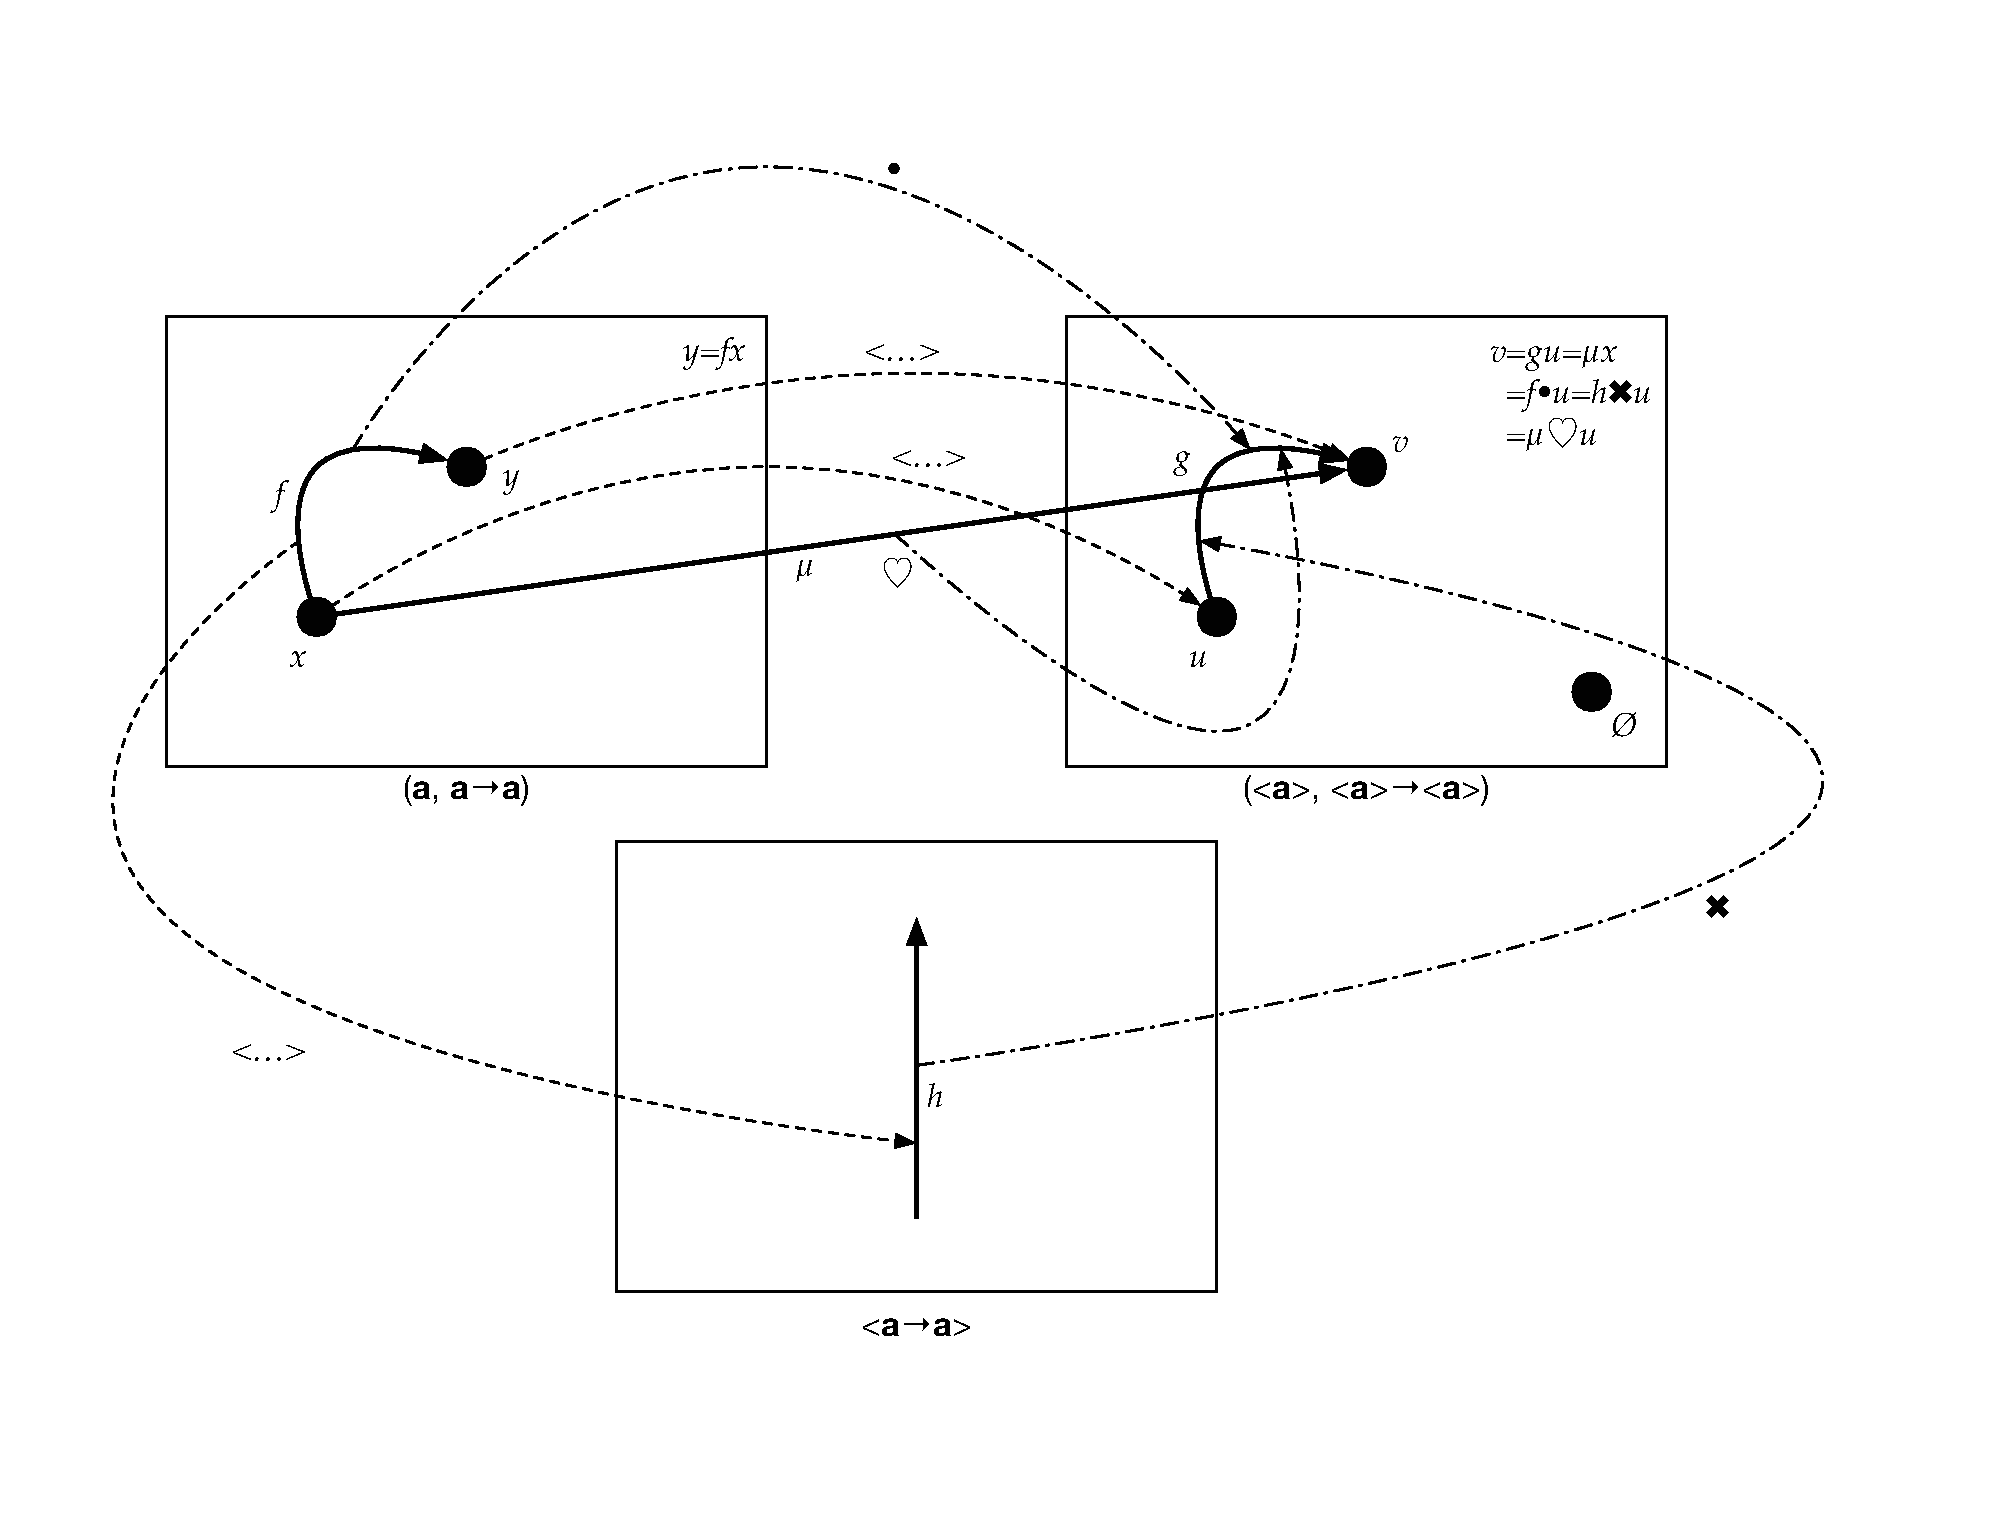
\includegraphics[width=100mm]{fig/functor.eps}
\end{center}
\caption{...}
\label{fig:functor}
\end{figure*}

% \section{IOモナド*}

\begin{table*}
\label{tab:monadplus}
\caption{型と型クラスの関係}
\begin{center}
\begin{tabular}{||c||c|c|c|c|c|c||}
\hline
\multirow{4}{*}{型$\backslash$型クラス}
  &\multicolumn{6}{|c||}{$\mMonadPlusTypeClass$}\\
\cline{2-7}
\multirow{3}{*}{}
  &\multicolumn{4}{|c|}{$\mMonadTypeClass$}
  &\multicolumn{2}{|c||}{$\mMonoidTypeClass$}\\
\cline{3-5}
\multirow{2}{*}{}
  &
  &\multicolumn{3}{|c|}{$\hTypeName{a}pplicativeTypeClass$}
  &\multicolumn{2}{|c||}{}\\
\cline{5-5}
\multirow{1}{*}{}
  &
  &\multicolumn{2}{|c|}{}
  &$\mFunctorTypeClass$
  &\multicolumn{2}{|c||}{}\\
\hline\hline
一般モノイド
  &
  &
  &
  &
  &$\mZero$
  &$\hAnyBinOp$\\
\hline
整数
  &
  &
  &
  &
  &$\hConstant{0}$
  &$+$\\
\hline
整数
  &
  &
  &
  &
  &$\hConstant{1}$
  &$*$\\
\hline\hline
一般コンテナ
  &$\hTypeName{b}ind$
  &$\mPureWith{x}$
  &$\hTypeName{a}ppMap$
  &$\mMap$
  &
  &\\
\hline
リスト
  &$\hTypeName{b}indList$
  &$[x]$
  &$\hTypeName{a}ppMapList$
  &$\hMap$
  &$\mEmptyList$
  &$\hAppend$\\
\hline
Maybe
  &$\hTypeName{b}indMaybe$
  &$\hJustWith{\hVar{x}}$
  &$\hTypeName{a}ppMapMaybe$
  &$\hMaybeMap$
  &$\hNothing$
  &($\hVar{x}$ の型に依存)\\
\hline
関数
  &$\hTypeName{b}indFunc$
  &$\mConstWith{x}$
  &$\hTypeName{a}ppMapFunc$
  &$\mMapFunc$
  &$\hAnonParam$
  &$\hCompose$\\
\hline
% \hline
% 記号
%   &\code{=<<}
%   &\code{pure}
%   &\code{fmap}
%   &\code{map}
%   &\\
% \hline
\end{tabular}
\end{center}
\end{table*}

\section{余談:モナドとしての関数}

関数はアプリカティブ関手であった.関数のピュア演算子とアプリカティブマップ演算子はそれぞれ
\begin{align}
\mConstWith{x}&=\hLambdaSyntax{\_}{\hVar{x}}\\
\hFunc{g}\hTypeName{a}ppMapFunc\hFunc{f}&=\hLambdaSyntax{\hVar{x}}{\hFunc{g}\hVar{x}(\hFunc{f}\hVar{x})}
\end{align}
であった.
% 関数ピュア演算子は,任意の引数 $\hVar{x}$ を関数に置き換える.ただし,その関数は引数を捨てて元の変数 $\hVar{x}$ を返す.例えば
% \begin{equation}
% x=\mFuncWith{x}y
% \end{equation}
% と,ダミー変数 $\hVar{y}$ を使って中身の $\hVar{x}$ を取り出せる.

関数のバインド演算子 $\hTypeName{b}indFunc$ を考えておこう.関数のバインド演算子は
\begin{equation}
g\hTypeName{b}indFunc f=\hLambdaSyntax{x}{g(\hFunc{f}\hVar{x})x}
\end{equation}
と定義する.ピュア演算子とバインド演算子から,関数のマップ演算子を
\begin{align}
\mConstWith{g\hAnonParam}\hTypeName{b}indFunc f
&=\hLambdaSyntax{x}{\mConstWith{g\hAnonParam}(\hFunc{f}\hVar{x})x}\\
&=\hLambdaSyntax{x}{\mConstWith{g(\hFunc{f}\hVar{x})}x}\\
&=\hLambdaSyntax{x}{(\hLambdaSyntax{\_}{g(\hFunc{f}\hVar{x})})x}\\
&=\hLambdaSyntax{x}{g(\hFunc{f}\hVar{x})}\\
&=\hFunc{g}\hCompose f\\
&=\hFunc{g}\mMapFunc f
\end{align}
のように合成できる.

まとめると
\begin{align}
\mConstWith{x}&=\hLambdaSyntax{\_}{x}\\
\hFunc{g}\mMapFunc\hFunc{f}&=\hLambdaSyntax{x}{g(\hFunc{f}\hVar{x})}=\hFunc{g}\hCompose f\\
\hFunc{g}\hTypeName{a}ppMapFunc\hFunc{f}&=\hLambdaSyntax{x}{\hFunc{g}\hVar{x}(\hFunc{f}\hVar{x})}\\
g\hTypeName{b}indFunc f&=\hLambdaSyntax{x}{g(\hFunc{f}\hVar{x})x}
\end{align}
である.

% ***Reason***
% http://south37.hatenablog.com/entry/2014/04/27/Haskell%E3%81%AB%E3%81%8A%E3%81%91%E3%82%8B%E3%83%A2%E3%83%8A%E3%83%89
% https://ja.wikipedia.org/wiki/%E3%83%A2%E3%83%8A%E3%83%89_(%E3%83%97%E3%83%AD%E3%82%B0%E3%83%A9%E3%83%9F%E3%83%B3%E3%82%B0)

\separator

関数はモノイドとしての性質も持つ.関数 $\mId=\hAnonParam$ とすると,任意の関数 $\hFunc{f}$ に対して
\begin{equation}
\mId\hCompose f=\hFunc{f}\hCompose\mId=\hFunc{f}
\end{equation}
であるから,関数全体の集合を $\mFSet$ で表すと,組み合わせ $(\mFSet,\hCompose,\mId)$ はモノイドである.

モナドでありモノイドである型クラスを\keyword{モナドプラス}と呼ぶ.関数はモナドプラスである.

今まで出てきた型と型クラスの関係を表\ref{tab:monadplus}に示す.Maybeに関しては $\hTypeName{a}$ 型がモノイドである場合に限って $\hMaybeConstruct{\hTypeName{a}}$ 型もモノイドである.

\section{この章のまとめ*}

\begin{enumerate}
\item ...
\end{enumerate}

% http://itpro.nikkeibp.co.jp/article/COLUMN/20120110/378061/

\chapter{IO*}
\label{ch:io}

A...

\section{アクション}

計算機の状態を変えることを\keyword{副作用}と呼ぶ.副作用とは変数への破壊的代入に他ならない.例えば,計算機は画面やプリンタに何かを出力するが,それは画面やプリンタという「変数」を書き換えていることになる.また例えば擬似乱数の生成も副作用である.呼び出されるたびに異なる値を返す擬似乱数生成関数は,そのたびに計算機の内部状態を書き換えているのである.

副作用を持つ関数を\keyword{アクション}と呼ぶ.アクションは値を持つが,その値は計算の実行時までわからない.例えば擬似乱数を生成するアクション $\mRand$ があるとしよう.これを変数 $\alpha$ に
\begin{equation}
\alpha=\mRand
\end{equation}
と代入しても,変数 $\alpha$ に擬似乱数が代入されるわけではない.「擬似乱数を生成する」というアクションが $\alpha$ に代入されたのだ.

では,いつ「擬似乱数を生成する」アクションが実行されるのだろうか.それは,プログラムがまさに計算機の状態を変えるタイミング,つまりプログラムが実行されるタイミングなのである.そのためには,プログラムそのものをアクションで表しておかないといけない.我々はプログラム全体を $\omega$ で表すことにしよう.

プログラムが計算機状態を変える一例として,画面に値を出力することを考える.画面に値を出力するアクションを $\mPutStr$ と名付けよう.例えば次のプログラム例は,画面に ``Hello, world.'' と書き出すものとする.
\begin{equation}
\omega=\mPutStr s\mWhereIsEXP{s}{\mString{``Hello, world.''}}
\end{equation}
アクション $\mPutStr$ は変数を一つとり,その値を画面へ出力すなち破壊的代入を行う.では $\omega=\mPutStr\alpha$ とすればアクション $\alpha$ が実行されて,晴れて擬似乱数が生成され,その値が画面へ出力されるだろうか.もちろんそうはならないのである.

ここに $\alpha$ はアクションであり,変数ではない.一方で,アクション $\mPutStr$ は変数を受け取る.つまり,アクションから何らかの方法で値を「安全に」抜き取らないといけない.ここで安全性にこだわるのは,アクション $\alpha$ が副作用を持つからである.副作用を参照透過な変数へ伝播させてはいけない.副作用を持つアクションは,副作用を持つアクションへのみ受け継がれなければならない.

この話は何かと似ていないだろうか.そう,Maybeである.一度ゼロ除算の可能性に汚染されたコンテナ変数は,コンテナから出すことが許されないのである.Maybeを返す関数$\hFunc{f}$の戻り値
\begin{equation}
  \begin{aligned}
    \hFunc{f}\hVar{x}&\hGuard{x\neq0}=\hJustWith{1/x}\\
    &\hGuard{\hOtherwise}=\hNothing
  \end{aligned}
\end{equation}
を,別の関数
\begin{equation}
  gy=1+y
\end{equation}
に渡そうと思ったら,
\begin{equation}
  g\hTypeName{b}ind \hFunc{f}\hVar{x}
\end{equation}
のようにバインド演算子で合成しなければならなかった.

我々はアクションにもバインド演算子を拡張して,
\begin{equation}
  \omega=\mPutStr\hTypeName{b}ind\alpha
\end{equation}
とする.これは第\ref{ch:monad}章で見たバインド演算子と同じものである.同じバインド演算子が使えるカラクリは,次節で見ていくことにする.

\section{IOモナド}

ある関数 $c$ が引数を取らず,いつも決まった $\hDouble$ 型の数を返すとしよう.そうすると,関数 $c$ の型は単純に $\hDouble$ である.

呼び出すたびに異なる擬似乱数を返すアクション $\mRand$ もまた毎回 $\hDouble$ 型の数を返す.そこで $\mRand$ も $\hDouble$ 型としたいところだが,こちらは関数ではなくアクションである.そこを区別するために,$\mRand$ の型は $\mIODoubleType$ 型と $\mIOType{\dotsb}$ に入れ
て区別する.\footnote{\haskell では $\mIODoubleType$ のことを \code{IO Double} と書く.}

呼び出しても何も返さないアクションはどのような型を持つべきだろう.何も返さない関数というものは無意味だが,アクションは副作用を持つので,何も返さないものがあっても良いのである.何も返さないことを「空っぽ」を返すと読み替えて,何も返さないアクションの型を $\mIOUnitType$ 型としよう.ここに $\mUnitType$ は「空っぽ」の意味で,ユニット型と読む.$\mIOUnitType$ 型のアクションの例は,画面に値を出力する $\mPutStr$ アクションである.\footnote{\haskell では $\mIOUnitType$ のことを \code{IO ()} と書く.}

キーボードからの入力を受け取るアクションもある.そのアクションを $\mReadLn$ としよう.アクション $\mReadLn$ は文字列型を返すので,その型は $\mIOStringType$ である.\footnote{\haskell では $\mIOStringType$ のことを \code{IO String} と書く.}

アクション $\mPutStr,\mReadLn,\mRand$ は計算機の状態を変化させる.アクション $\mPutStr,\mReadLn$ はOSのシステムコールを発行して,前者ならビデオメモリの値を書き換えるし,後者ならシリアルインタフェースの入力バッファをフラッシュする.アクション $\mRand$ は呼ばれるたびに内部のカウンタ値を一つ進める.これらのアクションは参照透過性を破壊する.そのために,プログラムの他の部分から隔離されねばならない.その隔離のメカニズムを提供するのがモナドである.

$\hListConstruct{\hTypeName{a}}$ 型が $\hTypeName{a}$ 型のリストであるように,$\mIOType{a}$ 型は $\hTypeName{a}$ 型の\keyword{IO}である.そしてリストがモナドであるように,IOもまたモナドである.モナドには,バインド演算子と,アプリカティブ関手から引き継いだピュア演算子の二つが必要であった.アプリカティブ関手から引き継いだアプリカティブマップ演算子はバインド演算子とピュア演算子の二つから合成できるし,関手から引き継いだマップ演算子もまたアプリカティブマップ演算子とピュア演算子から合成できるから,アプリカティブマップ演算子とマップ演算子は改めて実装しておく必要はない.

$\mIOUnitType$ 型の場合,ピュア演算子は何も返す必要がないから
\begin{equation}
\mPureWith{\_}=()
\end{equation}
であるとする.

% ここに $\hSingleTuppleWith{}$ は空のタプルで,「ユニット」と呼ぶ.一方で
% $\mIOUnitType$ 型のバインド演算子は,処理系の奥深くに隠されている.

% 実装依存である.


% http://tnomura9.exblog.jp/12069145/

\section{do記法}

モナドを使った書き方が従来のプログラムの記法からあまりにもかけ離れていることに,\haskell の設計者は気づいていたようで,\haskell には次に述べる\keyword{do記法}という記法が用意されている.このdo記法はもちろんシンタックスシュガーで,新しいことは何もない.

例えば $\omega=\mPutStr\hTypeName{b}ind\alpha\mWhereIsEXP{\alpha}{\mRand}$ をdo記法
を用いて書き直すと
\begin{equation}
\label{eq:do-print-random}
\omega=\mDo{a\mDoEq\mRand\mDoNext\mPutStr a}
\end{equation}
となる.ここで変数 $a$ は $\{\dotsb\}$ の中でだけ参照できる変数である.バインド演算子が副作用やゼロ除算汚染を中に閉じ込めたように,do記法の括弧は副作用や汚染を閉じ込める役割を果たす.\footnote{\haskell では \code{omega = do \{ a <- rand; putStr
a \}} と書くか,または $\mDoNext$ を改行に置き換えて
\begin{verbatim}
  omega = do
    a <- rand
    putStr a
\end{verbatim}
と書く.}

ここで,同様なことをする\python プログラムを見てみよう.
\begin{pythoncode}
\begin{verbatim}
import random
define main:
  a = random.random() # (1)
  print(a)            # (2)
\end{verbatim}
\end{pythoncode}
コード中の \code{(1)} の行で $a\mDoEq\mRand$ を実行し,\code{(2)} の行で $\mPutStr a$ を実行していると思えば,このコードと式\eqref{eq:do-print-random}の順序はそっくり同じである.もちろんこのdo記法はバインド演算子を使った式を切り貼りして,順序を入れ替えただけである.

do記法には $\mDoEq$ の他に,我々の $\mLetKeyword$ とよく似た $\mDoLetKeyword$ という構文が用意されている.この $\mDoLetKeyword$ は局所変数の導入に用いられて,例えば
\begin{equation}
\omega=\mDo{\mDoLet{y}{\hFunc{f}\hVar{x}}\mDoNext\alpha y}
\end{equation}
のように使う.

以下に,do記法を使った例を示す.
\begin{gather}
\mDo{\alpha x}=\alpha x\\
\mDo{y\mDoEq\alpha x\mDoNext\beta y}=\beta\hTypeName{b}ind\alpha x\\
\mDo{\alpha x\mDoNext\beta y}=(\hLambdaSyntax{\_}{\beta y})\hTypeName{b}ind \alpha x\label{eq:do-alpha-beta}\\
\mDo{\mDoLet{y}{\hFunc{f}\hVar{x}}\mDoNext\alpha y}=\alpha y\mWhereIsEXP{y}{\hFunc{f}\hVar{x}}\\
\mDo{y\mDoEq\alpha x\mDoNext\mDoLet{z}{fy}\mDoNext\beta z}
=\beta\hTypeName{b}ind{}(\hFunc{f}\mMap\alpha x)
\end{gather}
より複雑な例も挙げる.
\begin{multline}
\mDo{y\mDoEq\alpha x\mDoNext y'\mDoEq\alpha'x'\mDoNext\mDoLet{z}{fyy'}
\mDoNext\beta z}\\
=\beta\hTypeName{b}ind{}(\hFunc{f}\mMap\alpha x\hTypeName{a}ppMap\alpha'x')
\end{multline}
最後にdo記法中に変数を2回以上使いまわす例を示す.
\begin{multline}
\mDo{y\mDoEq\alpha x\mDoNext y'\mDoEq\alpha'x'\mDoNext\mDoLet{z}{fyy'}\mDoNext\beta z\mDoNext\mDoLet{z'}{f'yy'}\mDoNext\beta'z'}\\
=(\mLambda yy'\mLambdaArrow{}((\hLambdaSyntax{\_}{\mLetInEXP{z}{fyy'}{\beta z}})\\
\hTypeName{b}ind{}(\mLetInEXP{z'}{f'yy'}{\beta'z'}))) (\alpha x)(\alpha'x')
\end{multline}
この例では変数 $y,y'$ が2回使われている.

% なお $\mFuncWith{f}=\hLambdaSyntax{\_}{f}$ の関係を用いると式\eqref{eq:do-alpha-beta}はより簡潔に
% \begin{equation}
% \mDo{\alpha x\mDoNext\beta y}=\mFuncWith{\beta y}\hTypeName{b}ind\alpha x
% \end{equation}
% と書ける.

我々はバインド演算子を使った通常の記法とdo記法のいずれか読みやすい方を採用すれば良い.

% main =
% do
%   r <- rand
%   print r

% http://qiita.com/saltheads/items/6025f69ba10267bbe3ee

\separator

バインド演算子には,左右の引数を入れ替えた\keyword{右バインド演算子}がある.右バインド演算子は $\hTypeName{b}indRight$ と書き,
\begin{equation}
\alpha x\hTypeName{b}indRight\beta=\beta\hTypeName{b}ind\alpha x
\end{equation}
であるとする.\footnote{\haskell では $\alpha x\hTypeName{b}indRight\beta$ を \code{alpha x >>= beta} と書く.}

\section{余談:関数であるということ*}

IOモナドの変数は,たとえ値を読み出すだけであっても必ず関数適用が必要である.それは,IOモナドの変数が「自分が読み出されたこと」を知る必要があるからである.IOモナドの変数は,自分が読み出されたタイミングで副作用を発生させる.これは\objectivec や\swift に見られる getter メソッドと同じ考え方である.

IOモナドの変数値を読み出すために行われる関数呼び出しはダミーである場合があり,戻り値はしばしば捨てられる.

変数をダミーの関数で包み,それをさらにIOモナドで包んだのがIOモナド変数である.

もうひとつ,アクションが関数でなければならない理由がある.\haskell はいつも遅延評価を行うことを思い出してもらいたい.\python であれば,式は書かれた順に評価される.しかし,例えば
\begin{align}
y_1&=\hFunc{f} \hVar{x}_1\\
y_2&=\hFunc{g} \hVar{x}_2
\end{align}
という式があった場合,関数 $\hFunc{f}$ と $\hFunc{g}$ のどちらが先に評価されるか,あるいは同時に評価されるかは\haskell では未定義である.\haskell で唯一計算順序が保証されているのは,関数適用である.例えば
\begin{equation}
y=\hFunc{g}_2(g_1x)
\end{equation}
であれば,確実に関数 $g_1$ が関数 $g_2$ よりも先に評価される.

直列に評価したい関数の戻り値が,いつも次の関数の引数の型と一致しているとは限らないし,次の関数(アクション)が引数を取らない可能性もある.もし関数 $g_2$ が引数を取らなければ
\begin{equation}
\mConstWith{g_2}(g_1x)
\end{equation}
とする.この時,関数適用 $(g_1x)$ の結果は単純に捨てられる.
\footnote{\clang では \code{void} 型を返す関数 \code{void g1(int)} を引数を取らない関数 \code{int g2(void)} に「食わせる」ことが可能で,\code{g2(g1(x))} は正しいコードである.もっとも\clang プログラマは \code{g1(x), g2()} という書き方の方を好むであろう.}

\separator

ふたつのアクション $\alpha_1,\alpha_2$ があり,アクション $\alpha_2$ が引数を取らない場合,その二つを合成するには
\begin{equation}
\label{eq:ignore-return}
\alpha_1 x\hTypeName{b}indRight\mConstWith{\alpha_2}
\end{equation}
とする.式\eqref{eq:ignore-return}はしばしば
% \begin{equation}
% g_2\twoheadleftarrow g_1x=\mFuncWith{g_2}(g_1x)
% \end{equation}
% または
\begin{equation}
\alpha_1 x\hTypeName{b}indRightIgnore\alpha_2=\alpha_1x\hTypeName{b}indRight\mConstWith{\alpha_2}
\end{equation}
なる演算子 $\hTypeName{b}indRightIgnore$ を用いて記述される.\footnote{\haskell では $\alpha_1x\hTypeName{b}indRightIgnore\alpha_2$ を \code{alpha1 x >> alpha2} と書く.}

\section{この章のまとめ*}

\begin{enumerate}
\item do記法.
\end{enumerate}

\chapter{データ型の定義*}
\label{ch:data-type}

\section{データ型}

我々はしばしば新しい集合を考える必要に迫られる.例えば,イチ,ニ,サン,タクサンからなる集合
\begin{equation}
\mSet{Num}\mDefEq\{\mNumOne,\mNumTwo,\mNumThree,\mNumMany\}
\end{equation}
を考えることがあるだろう.集合 $\mSet{Num}$ の元 $n\hIsTypeOf\mSet{Num}$ は $\mNumOne$, $\mNumTwo$, $\mNumThree$, $\mNumMany$ のいずれかの値を取ることになる.

数学者は新しい集合を定義するが,\haskell プログラマは新しいデータ型を定義する.集合 $\mSet{Num}$ の定義の代わりに,我々はデータ型
$\mType{Num}$ を
\begin{equation}
  \mDataType\;\mType{Num}
  =\mNumOne\mValueOr\mNumTwo\mValueOr\mNumThree\mValueOr\mNumMany
\end{equation}
のように書いて定義するものとする.式の先頭にある $\mDataType$ は,この式がデータ型の定義であることを示すタグである.部分的にアンダーラインが引かれているのは,\haskell が $\mDataType$ を \code{data} と省略してしまうからである.これは不本意なことだが,文字数節約のために仕方ない.ここに $\mSet{Num}$ は型コンストラクタ,$\mNumOne$, $\mNumTwo$, $\mNumThree$, $\mNumMany$ は値コンストラクタである.\footnote{\haskell では \code{data Num = One | Two | Three | Many} と書
  く.}

% 値コンストラクタを列挙したデータ型を\keyword{代数型}と呼ぶ.

この節で紹介したデータ型の定義は\clang で言う \code{enum} に近い.他に\clang で言う \code{struct} や \code{union} すなわち構造体や共用体もこの $\mDataType$ 文で定義できるが,これは次節で見ることにする.

\separator

新しいデータ型がある型クラスに属すとき,$\mDataType$ 文でそれを同時に宣言できる.例えば $\mType{Num}$ 型は同値演算子 $(\hIfEq)$ を持つことが自然である.型 $\mType{Num}$ が $\hEq$ 型クラスに属すとき,
\begin{equation}
  \mDataType\;
  \mType{Num}
  =\mNumOne\mValueOr\mNumTwo\mValueOr\mNumThree\mValueOr\mNumMany
  \mDeriving\hEq
\end{equation}
のように書く.\footnote{\haskell では \code{data Num = One | Two | Three | Many deriving Eq} と書く.}

型 $\mType{Num}$ の同値演算子 $(\hIfEq)$ の実装は\ref{sec:type-class-and-instance}節で見ることにする.

\section{レコード構文}

データ型の定義では,値コンストラクタにパラメタを与えることもできる.例えば $\mType{Rectangle}$ という型を考えよう.この型は,始点の平面座標と幅,高さで合計4個の $\hFloat$ のパラメタを取るものとする.このとき
\begin{multline}
  \label{eq:rectangle}
  \mDataType\;
  \mType{Rectangle}\\
  =\mValueWith{Rectangle}
  {\hFloat\,\hFloat\,\hFloat\,\hFloat}
  \mDeriving\hEq
\end{multline}
という風にデータ型の定義を行う.\footnote{\haskell では \code{data Rectangle = Rectangle Float Float Float Float} と書く.}

$\mType{Rencatngle}$ 型の変数は次のように初期化する.
\begin{equation}
  \left\{
  \begin{aligned}
    r&\hIsTypeOf\mType{Rectangle}\\
    r&=\mValueWith{Rectangle}{1\,2\,3\,4}
  \end{aligned}
  \right.
\end{equation}
これは\clang で言う \code{struct} と似た用法である.\footnote{\haskell では
\begin{verbatim}
  r :: Rectangle
  r = Rectangle 1 2 3 4
\end{verbatim}
と書く.}

$\mType{Rectangle}$ 型から中身を取り出すには,次のような関数を用意しておかねばならない.
\begin{align}
  x\,\mValueWith{Rectangle}{a\,\_\,\_\,\_}
  &=a\\
  y\,\mValueWith{Rectangle}{\_\,a\,\_\,\_}
  &=a\\
  width\,\mValueWith{Rectangle}{\_\,\_\,a\,\_}
  &=a\\
  height\,\mValueWith{Rectangle}{\_\,\_\,\_\,a}
  &=a
\end{align}
この面倒は,次のシンタックスシュガーを使うことで軽減される.
\footnote{\haskell では
\begin{verbatim}
  x      Rectangle a _ _ _ = a
  y      Rectangle _ a _ _ = a
  width  Rectangle _ _ a _ = a
  height Rectangle _ _ _ a = a
\end{verbatim}
と書く.}

型 $\mType{Rectangle}$ のようにパラメタが多いときは,パラメタに名前があると便利である.そこで利用できるのが\keyword{レコード構文}である.レコード構文を使うと,式\eqref{eq:rectangle}は
\begin{multline}
  \mDataType\;\mType{Rectangle}\\
  =\mValueRecordBeginWith{Rectangle}
  x\hIsTypeOf\hFloat,
  y\hIsTypeOf\hFloat,
  width\hIsTypeOf\hFloat,
  height\hIsTypeOf\hFloat
  \mValueRecordEnd\\
  \mDeriving\hEq
\end{multline}
のように書き直すことができる.\footnote{\haskell では
\begin{verbatim}
  data Rectangle = Rectangle {
      x      :: Float,
      y      :: Float,
      width  :: Float,
      height :: Float
    }
    deriving Eq
\end{verbatim}
と書く.}

レコード構文を用いると,型から中身を取り出す関数は自動的に定義される.また
\begin{equation}
  r=
  \mValueRecordWith{Rectangle}{
    x=1,
    y=2,
    width=3,
    height=4
  }
\end{equation}
のようなレコード構文専用の初期化を行っても良いし,従来の初期化方法を用いても良い.\footnote{\haskell では\code{r = Rectangle \{ x = 1, y = 2, width = 3, height = 4 \}} と書く.}

\separator

データ型の定義には,複数の値コンストラクタを指定できる.そのため
\begin{multline}
\mDataType\;\mType{Shape}
=\mValueWith{Circle}{\hFloat\,\hFloat}\\
\mValueOr
\mValueWith{Triangle}{\hFloat\,\hFloat\,\hFloat}
\end{multline}
のようなデータ型の定義も可能である.この例では型 $\mType{Shape}$ は値コンストラクタ $\mValueConstructor{Circle}$ または $\mValueConstructor{Triangle}$ によって初期化され,それぞれ2個または3個の $\hFloat$ 型のパラメタを取る.\footnote{\haskell では \code{data Shape = Circle Float Float | Triangle Float Float Float} と書く.}

\section{型クラスとインスタンス化}
\label{sec:type-class-and-instance}

型クラスとは,複数の型が持つ共通のインタフェースである.その複数の型をいま $\hTypeName{a}$ で表すこととして,型 $\hTypeName{a}$ が型クラス$\hEq$ に属すとしよう.型クラス $\hEq$ は等号$(\hIfEq)$ と不等号 $(\neq)$ をインタフェースとして持つ.このことを
\begin{equation}
  \mTypeClassDecl\hTypeName{a}thop{\hEq}\hHasElementsOf\hTypeName{a}\mWhere{}
  \left\{
  \begin{aligned}
    &(\hIfEq)\hIsTypeOf\mProjEXP{\hTypeName{a} }{\mProjEXP{\hTypeName{a} }{\hBool}}\\
    &(\neq)\hIsTypeOf\mProjEXP{\hTypeName{a} }{\mProjEXP{\hTypeName{a} }{\hBool}}\\
    &x\hIfEq y=\neg(x\neq y)\\
    &x\neq y=\neg(x\hIfEq y)
  \end{aligned}
  \right.
\end{equation}
と書く.\footnote{\haskell では$\mTypeClassDecl$ を \code{class} と書く.また $\hHasElementsOf$ を省略して,
\begin{verbatim}
  class Eq a where
    (==) :: a -> a -> Bool
    (/=) :: a -> a -> Bool
    x==y = not(x/=y)
    x/=y = not(x==y)
\end{verbatim}
と書く.}

\TK{$\mTypeClassDecl$ による具象型の型クラス宣言.}

ここで宣言したのは等号,不等号というインタフェースが「ある」という事だけで,その実装は未定義である.等号,不等号の実装は次に述べる $\mInstanceDecl$ 文を使う.

型クラス $\hEq$ に属す型 $\hTypeName{a}$ は等号と不等号を持つ.我々の型 $\mType{Num}$ が型クラス $\hEq$ に属すことを宣言し,型クラス $\hEq$ が備えるべき等号,不等号を実装するには
\begin{equation}
  \mInstanceDecl\;\hEq\hHasElementsOf\mType{Num}
  \mWhere{}
  \left\{
  \begin{aligned}
    \mNumOne\hIfEq\mNumOne&=\hTrue\\
    \mNumTwo\hIfEq\mNumTwo&=\hTrue\\
    \mNumThree\hIfEq\mNumThree&=\hTrue\\
    \mNumMany\hIfEq\mNumMany&=\hTrue\\
    \_\hIfEq\_&=\hFalse
  \end{aligned}
  \right.
\end{equation}
とする.これを\keyword{型クラスのインスタンス化}と呼ぶ.
\footnote{\haskell では
\begin{verbatim}
  instance Eq Num where
    One==One     = True
    Two==Two     = True
    Three==Three = True
    Many==Many   = True
    _==_         = False
\end{verbatim}
と書く.}

\TK{$\mInstanceDecl$ による具象型のインスタンス宣言.}

型クラスは\keyword{継承関係}を持てる.型クラス $\hOrd$ は型クラス $\hEq$ から等号,不等号を継承し「小なりイコール」 $(\le)$ を追加する.
\begin{equation}
  \mTypeClassDecl\;\hEq\hHasElementsOf\hTypeName{a}
  \hAndThen\hTypeName{a}thop{\hOrd}\hHasElementsOf\hTypeName{a}
  \mWhere{}(\le)\hIsTypeOf\mProjEXP{\hTypeName{a} }{\mProjEXP{\hTypeName{a} }{\hBool}}
\end{equation}
型クラス $\hOrd$ に属する型は,等号,不等号,小なりイコールと,それらから派生させることのできる大なり $(>)$,大なりイコール $(\ge)$,小なり $(<)$,および最大値をとる関数 $\hTypeName{a}x$ と最小値をとる関数 $\hIsTypeOf$を持つ.\footnote{\haskell では
\begin{verbatim}
  class (Eq a) => Ord a where (<=) :: a -> a -> Bool
\end{verbatim}
と書く.}

\separator

型は複数の型クラスに同時に属すことができる.例えば型 $\mType{Num}$ は型クラス $\hEq$ と同時に型クラス $\hOrd$ に属すこともできる.それには
\begin{equation}
\mDataType\;\mType{Num}
=\mNumOne\mValueOr\mNumTwo\mValueOr\mNumThree\mValueOr\mNumMany
\mDeriving{}(\hEq,\hOrd)
\end{equation}
とする.\footnote{\haskell では
\begin{verbatim}
  data Num = One | Two | Three | Many deriving (Eq, Ord)
\end{verbatim}
と書く.}

型クラス $\hOrd$ のインスタンスは小なりイコール演算子 $(\le)$ が定義されていなければならない.我々は
\begin{equation}
  \mInstanceDecl\;\hOrd\hHasElementsOf\mType{Num}
  \mWhere{}
  \left\{
  \begin{aligned}
    \mNumOne\le\mNumOne&=\hTrue\\
    \mNumOne\le\mNumTwo&=\hTrue\\
    \mNumOne\le\mNumThree&=\hTrue\\
    \mNumOne\le\mNumMany&=\hTrue\\
    \mNumTwo\le\mNumTwo&=\hTrue\\
    \mNumTwo\le\mNumThree&=\hTrue\\
    \mNumTwo\le\mNumMany&=\hTrue\\
    \mNumThree\le\mNumThree&=\hTrue\\
    \mNumThree\le\mNumMany&=\hTrue\\
    \mNumMany\le\mNumMany&=\hTrue\\
    \_\le\_&=\hFalse
  \end{aligned}
  \right.
\end{equation}
のように $\mType{Num}$ の $\le$ 演算子を定義することができる.

\section{余談:レンズ*}

\TK{Lens}

% \section{余談:型シノニム*}

---

\TK{Move to 12.4}

データ型には\keyword{シノニム}(別名)がつけられる.例えば $\hChar$ のリスト $[\hChar]$ は
\begin{equation}
  \mTypeSynonymDecl\;
  \mStringType
  =[\hChar]
\end{equation}
とすることで,別名 $\mStringType$ を与えることができる.\haskell では$\mTypeSynonymDecl$ を \code{type} と省略してしまう.これは残念なことだが,\clang の \code{typedef} のようなものだと思って割り切るしかない.\footnote{\haskell では \code{type String = [Char]} と書く.}

\section{この章のまとめ*}

\begin{enumerate}
\item ...
\end{enumerate}

\begin{note}{メタクラス}
オブジェクト指向言語の多くが「クラス」と呼ぶものを,\haskell は「型」と呼ぶ.

% クラスのクラスをメタクラスと言う.

% メタクラスのクラスはメタメタクラスである.全てのメタクラスはメタメタクラスに属す.それ故,メタメタクラスもまたメタメタクラスに属す.
\end{note}


\chapter{多相型の定義*}
\label{ch:polymorphic-data-type}
...

\section{多相型}

Maybeのように型パラメタを取る型を\keyword{多相型}と呼ぶ.多相型はどのように定義されるかと言うと,
\begin{equation}
  \mDataTypePolymorphic\;
  \hMaybe\,\hTypeName{a}
  =\hJustWith{\hTypeName{a}}\mValueOr\hNothing
\end{equation}
のように,やはり $\mDataType$ を使って定義される.念のため型パラメタを取る場合は $\mDataTypePolymorphic$ と区別しておこう.\footnote{\haskell は $\mDataType$ と $\mDataTypePolymorphic$ を区別せず,$\mDataTypePolymorphic\;\hMaybe\hTypeName{a}=\hJustWith{\hTypeName{a} }\mValueOr\hNothing$ を \code{data Maybe a = Just a | Nothing} と書く.}
% この $\hJustWith{\hTypeName{a}}$ は $\hTypeName{a}$ のMaybe型 $(\hMaybeConstruct{\hTypeName{a}})$ という
% 意味ではなく,$\hTypeName{a}$ 型の変数を型コンストラクタ $\hJustWith{\dotsb}$
% に入れなさいという意味.

Maybeが型クラス $\hEq$ に属すものとして,$\hEq$ からのインスタンス化をしておこう.ここでも型パラメタ付きの $\mInstanceDecl$ を仮に $\mInstanceDeclPolymorphic$ とすると次のように書けそうである.
\begin{equation}
  \mInstanceDeclPolymorphic\;
  \hEq\hHasElementsOf{}(\hMaybe\,\hTypeName{a})
  \mWhere
  \left\{
  \begin{aligned}
    \hJustWith{\hVar{x}}\hIfEq\hJustWith{y}
    &=x\hIfEq y\\
    \hNothing\hIfEq\hNothing
    &=\hTrue\\
    \_\hIfEq\_
    &=\hFalse
  \end{aligned}
  \right.
\end{equation}
残念ながら,この式は $\hTypeName{a}$ 型の変数 $\hVar{x},\hVar{y}$ の間に等号 $(\hIfEq)$ が定義されていることが隠れた前提になっているため,正しくない.我々は $\hTypeName{a}$ が型クラス $\hEq$ に属すことを要求するので,次のように言い換える.
\begin{multline}
\mInstanceDeclPolymorphic\;
\hEq\hHasElementsOf\hTypeName{a}
\hAndThen
\hEq\hHasElementsOf{}(\hMaybe\,\hTypeName{a} )\\
\mWhere
\left\{
\begin{aligned}
\hJustWith{\hVar{x}}\hIfEq\hJustWith{y}&=x\hIfEq y\\
\hNothing\hIfEq\hNothing&=\hTrue\\
\_\hIfEq\_&=\hFalse
\end{aligned}
\right.
\end{multline}
この $\hEq\hHasElementsOf\hTypeName{a} \hAndThen$ の部分が「以下 $\hTypeName{a}$ 型は $\hEq$ 型クラスに属すものとして」という意味になる.\footnote{\haskell では
\begin{verbatim}
  instance Eq a => Eq (Maybe a) where
    Just x == Just y = x==y
    Nothing==Nothing = True
    _==_             = False
\end{verbatim}
と書く.}

Maybeの間に新たに定義された等号 $(\hIfEq)$ は次の型を持つ.
\begin{equation}
(\hIfEq)
\hIsTypeOf{}\hEq\hHasElementsOf\hTypeName{a}
\hAndThen\mProjEXP{\hMaybeConstruct{\hTypeName{a}}}{\mProjEXP{\hMaybeConstruct{\hTypeName{a}}}{\hBool}}
\end{equation}

\separator

多相型を定義するとき,型パラメタは2個以上与えられても良い.例えばEitherは次のように定義できる.
\begin{equation}
\mDataTypePolymorphic\;\hEither\,\hTypeName{a} \,\hTypeName{b}
=\hLeftWith{\hTypeName{a} }
\mValueOr
\hRightWith{\hTypeName{b} }
\end{equation}

\section{自己参照型}

型の定義中に自分自身を参照する型を\keyword{自己参照型}または
\keyword{再帰型}と呼ぶ.例えばリストは
\begin{equation}
\mDataTypePolymorphic\;\mListTypeConstructor\,\hTypeName{a} =\mEmptyList\mValueOr\hTypeName{a} :\mListTypeConstructor\,\hTypeName{a}
\end{equation}
のように定義できる.

\section{関手の拡張}

\TK{Writing.}

\begin{equation}
  \mTypeClassDeclPolymorphic\;
  \mFunctorTypeClass\hHasElementsOf\mTypeConstructor{f}
  \mWhere{}
  (\mMap)
  \hIsTypeOf{}(\hTypeName{a}\hFunctionArrow\hTypeName{b})
  \hFunctionArrow\mPolymorphicTypeAssemble{f}{a}
  \hFunctionArrow\mPolymorphicTypeAssemble{f}{b}
\end{equation}

\TK{$\mTypeClassDeclPolymorphic$ による型コンストラクタの型クラス宣言.}

型クラス $\mFunctorTypeClass$ はマップ演算子 $(\mMap)$ を提供する.リ
スト型は $\mFunctorTypeClass$ 型クラスのインスタンスなので,
\begin{equation}
  \mInstanceDeclPolymorphic\;
  \mFunctorTypeClass\hHasElementsOf\mListTypeConstructor{}
  \mWhere{}
  (\mMap)
  =(\hMap)
\end{equation}
と定義する.\footnote{\haskell では
\begin{verbatim}
  instance Functor [] where fmap = map
\end{verbatim}
と書く.}

\TK{$\mInstanceDeclPolymorphic$ による型コンストラクタのインスタンス宣言.}

\TK{Follow:} That's it! Notice how we didn't write instance Functor
   [a] where, because from fmap :: (a $\hTypeName{a}psto$ b) $\hTypeName{a}psto$ f a
   $\hTypeName{a}psto$ f b, we see that the f has to be a type constructor that
   takes one type. [a] is already a concrete type (of a list with any
   type inside it), while [] is a type constructor that takes one type
   and can produce types such as [Int], [String] or even [[String]].

Maybe型の場合は
\begin{equation}
  \mInstanceDeclPolymorphic\;
  \mFunctorTypeClass\hHasElementsOf\hMaybe
  \mWhere\left\{
  \begin{aligned}
    \hFunc{f}\mMap{}\hJustWith{\hVar{x}}&=\hJustWith{\hFunc{f}\hVar{x}}\\
    \hFunc{f}\mMap\hNothing&=\hNothing
  \end{aligned}
  \right.
\end{equation}
となる.\footnote{\haskell では
\begin{verbatim}
  instance Functor Maybe where
    fmap f (Maybe x) = Maybe (f x)
    fmap f Nothing = Nothing
\end{verbatim}
と書く.}

Either型の場合は
\begin{equation}
  \mInstanceDeclPolymorphic\;
  \mFunctorTypeClass\hHasElementsOf{}(\hEither\,\hTypeName{a})
  \mWhere{}
  \left\{
  \begin{aligned}
    \hFunc{f}\mMap{}\hRightWith{x}&=\hRightWith{\hFunc{f}\hVar{x}}\\
    \hFunc{f}\mMap{}\hLeftWith{x}&=\hLeftWith{x}
  \end{aligned}
  \right.
\end{equation}
となる.\footnote{\haskell では
\begin{verbatim}
  instance Functor (Either a) where
    fmap f (Right x) = Right (f x)
    fmap f (Left x)  = Left x
\end{verbatim}
と書く.}

\TK{Multiple parameter extension.}

\section{余談: \code{newtype}*}

リストに新しいマップ演算子 $\mZip$ を定義したいとしよう.この演算子 $\mZip$ は
\begin{equation}
  [\hFunc{f},\hFunc{g},\mHFunc]\mZip[x,\hVar{y},\hVar{z}]
  =[\hFunc{f}\hVar{x},gy,hz]
\end{equation}
のように働くとする.新しいマップ演算子 $\mZip$ のことを我々は\keyword{ジップ演算子}と呼ぶことにする.

ジップ演算子を定義するにはどうしたら良いだろうか.汎用性を考えると,ジップ演算子もまたリストのアプリカティブマップ演算子であって欲しい.ところが,リストには既に $\hTypeName{a}ppMapList$ というアプリカティブマップ演算子が定義されている.念のためにアプリカティブマップ演算子を用いると
\begin{equation}
  [\hFunc{f},\hFunc{g},\mHFunc]\hTypeName{a}ppMapList[x,\hVar{y},\hVar{z}]
  =[\hFunc{f}\hVar{x},\hFunc{f}\hVar{y},\hFunc{f}\hVar{z},\hFunc{g}\hVar{x},\hFunc{g}\hVar{y},\hFunc{g}\hVar{z},\mHFunc\hVar{x},\mHFunc\hVar{y},\mHFunc\hVar{z}]
\end{equation}
である.ある型のインスタンス化は一種類しか行えないので,リスト型に新しいアプリカティブマップ演算子を追加することは出来ない.

そこで $\mDataTypePolymorphic$ を使ってリスト型をラップした新しい型を作る.例えば新しい型を $\mZipListType{a}$ とすると
\begin{equation}
  \label{eq:data-type-ziplist}
  \mDataTypePolymorphic\;
  \hTypeName{a}thop{\mZipListTypeConstructor}\hTypeName{a}
  =\mValueRecordWith{ZipList}{\mGetList\hIsTypeOf{}\hListConstruct{\hTypeName{a}}}
\end{equation}
のように定義することになる.念のため,左辺の $\mZipListTypeConstructor$ は型コンストラクタ,右辺の $\mValueConstructor{ZipList}$ は値コンストラクタである.すなわち
\begin{equation}
  \mZipListType{a}
  =\mZipListTypeConstructor\hTypeName{a}
\end{equation}
である.

こうしておいて,あとは
\begin{multline}
  \mInstanceDeclPolymorphic\;
  \mFunctorTypeClass\hHasElementsOf\mZipListTypeConstructor\\
  \mWhere
  \hFunc{f}\mMap{}\mZipListWith{\hListVar{x}}=\mZipListWith{\hFunc{f}\hMap\hListVar{x}}
\end{multline}
および
\begin{multline}
  \mInstanceDeclPolymorphic\;
  \hTypeName{a}pplicativeTypeClass\hHasElementsOf\mZipListTypeConstructor\\
  \mWhere
  \left\{
  \begin{aligned}
    \mPureWith{x}
    &=\mZipListWith{\mRepeat x}\\
    \mZipListWith{\hListVar{f}}\hTypeName{a}ppMap\mZipListWith{\hListVar{x}}
    &=\mZipListWith{\hListVar{f}\mZip\hListVar{x}}
  \end{aligned}
  \right.
\end{multline}
と定義する.ここで
\begin{equation}
  \label{eq:zip}
  \left\{
  \begin{aligned}
    (\mZip)\_\mEmptyList&=\mEmptyList\\
    (\mZip)\mEmptyList\_&=\mEmptyList\\
    (\mZip)(\hVar{x}:\hListVar{x})(y:\hListVar{y})&=(x\hApply y):\hListVar{x}\mZip\hListVar{y}
  \end{aligned}
  \right.
\end{equation}
であると定義する.

関数 $\mRepeat$ は引数を無限回繰り返すリストを返す関数である.念のため関数 $\mRepeat$ の実装方法を書いておくと
\begin{equation}
  \left\{
  \begin{aligned}
    &\mRepeat\hIsTypeOf{}\mProjEXP{\hListConstruct{\hTypeName{a}}}{\hListConstruct{\hTypeName{a}}}\\
    &\mRepeat x=\hVar{x}:\mRepeat x
  \end{aligned}
  \right.
\end{equation}
である.

任意のリスト $\hListVar{x}$ と任意の関数リスト $\hListVar{f}$ ただし
\begin{align}
\hListVar{x}&=[\hVar{x}_0,\hVar{x}_1,\dotsb]\\
\hListVar{f}&=[\hFunc{f}_0,\hFunc{f},\dotsb]
\end{align}
の両方をそれぞれ値コンストラクタで包んでアプリカティブマップ演算子を適用すると
\begin{equation}
  \mZipListWith{\hListVar{f}}\hTypeName{a}ppMap\mZipListWith{\hListVar{x}}
  =[\hFunc{f}_0\hVar{x}_0,\hFunc{f} \hVar{x}_1,\dotsb]
\end{equation}
のようにジップ演算子を適用できる.

このままでも問題はないのだが,式\eqref{eq:data-type-ziplist}を次のように書き換えることがより好ましい.
\begin{equation}
  \mNewTypeDeclPolymorphic\;
  \mZipListTypeConstructor\hTypeName{a}
  =\mZipListRecordWith{\mGetList\hIsTypeOf{}\hListConstruct{\hTypeName{a}}}
\end{equation}
やったことはキーワード $\mDataTypePolymorphic$ を
$\mNewTypeDeclPolymorphic$ に置き換えたことである.これは,字面に反して,型 $\mZipListType{a}$ が何一つ「新しくない」ことを\haskell コンパイラに伝えるためである.その結果\haskell コンパイラは型 $\mZipListType{a}$ に対する最適化の機会を得る.

\separator

式\eqref{eq:zip}にもう一段の抽象化をしておこう.関数 $\mZipWith$ を
\begin{equation}
  \left\{
  \begin{aligned}
    {}&\mZipWith\hIsTypeOf{}\mProjEXP{\mProjEXP{\mProjEXP{(\mProjEXP{\hTypeName{a} }
          {\mProjEXP{\hTypeName{b} }{\mC }})}
        {\hListConstruct{\hTypeName{a}}}}{[\hTypeName{b}]}}{[\mC]}\\
    {}&\left\{\begin{aligned}
    \mZipWith\_\mEmptyList\_
    &=\mEmptyList\\
    \mZipWith\_\_\mEmptyList
    &=\mEmptyList\\
    \mZipWith f(\hVar{x}:\hListVar{x})(y:\hListVar{y})
    &=\hFunc{f}\hVar{x}\hVar{y}:\mZipWith f\hListVar{x}\hListVar{y}
    \end{aligned}
    \right.
  \end{aligned}
  \right.
\end{equation}
と定義する.こうすれば,演算子 $\mZip$ は
\begin{equation}
  (\mZip)
  =\mZipWith(\hApply)
\end{equation}
と関数 $\mZipWith$ から定義できる.

関数 $\mZipWith$ を再帰的に定義したが,再帰をリストのマップ演算子に押し込むこともできる.それには
\begin{equation}
  \mZipWith f(\hVar{x}:\hListVar{x})(y:\hListVar{y})
  =\hFunc{f}'\hMap\hListVar{z}
  \mWhere
  \left\{
  \begin{aligned}
    f'
    &\mLetEq\hUncurry f\\
    \hListVar{z}
    &\mLetEq\mZipFunc\hListVar{x}\hListVar{y}
  \end{aligned}
  \right.
\end{equation}
と,先に $\mZipFunc$ 関数を定義しておいて,その後 $\mZipWith$ 関数を定義する.ここに $\mZipFunc$ 関数は
\begin{equation}
  \left\{
  \begin{aligned}
    {}&\mZipFunc\hIsTypeOf{}\mProjEXP{\hListConstruct{\hTypeName{a}}}
    {\mProjEXP{[\hTypeName{b}]}
      {(\hListConstruct{\hTypeName{a}},[\hTypeName{b}])}}\\
    {}&\mZipFunc \hVar{x}\hVar{y}=(x,y)
  \end{aligned}
  \right.
\end{equation}
であり,$\hUncurry$ 関数は
\begin{equation}
  \left\{
  \begin{aligned}
    {}&\hUncurry\hIsTypeOf{}
    \mProjEXP{(\mProjEXP{\hTypeName{a} }{\mProjEXP{\hTypeName{b} }{\mC }})}
          {\mProjEXP{(\hTypeName{a} ,\hTypeName{b} )}{\mC }}\\
          {}&\hUncurry f\hVar{x}\hVar{y}=\hFunc{f}(x,y)
  \end{aligned}
  \right.
\end{equation}
である.\footnote{\haskell では $\mZipWith$ 関数を
\begin{verbatim}
  zipWith :: (a -> b -> c) -> [a] -> [b] -> [c]
  zipWith f (\hVar{x}:xs) (y:ys) = f' `map` zs where
    f' = uncurry f
    zs = zip xs ys
\end{verbatim}
と書ける.ただし \code{zipWith} は \filename{Prelude} から提供される.}

% http://haskell.g.hatena.ne.jp/hyuki/20060603/zipwith

\section{この章のまとめ*}

\begin{enumerate}
\item ...
\end{enumerate}

\chapter{カテゴリ*}
\label{ch:category}

\section{多値*}

\haskell の関数の引数は常にひとつであり,戻り値も常にひとつである.しか
し,複数の戻り値を返したい場合もある.例えば実数 $\hVar{x}$ の平方根は
$\sqrt{x}$ および $-\sqrt{x}$ のふたつである.そこで次のような関数
$\mSqrts$ ただし
\begin{equation}
  \left\{
  \begin{aligned}
    &\mSqrts\hIsTypeOf{}\hReal\hHasElementsOf\hTypeName{a} \hAndThen
    \hTypeName{a}\hFunctionArrow\hListConstruct{\hTypeName{a}}\\
    &\mSqrts x=[\mSqrt x,(-\mSqrt x)]
  \end{aligned}
  \right.
\end{equation}
を考えてみる.\footnote{\haskell では
\begin{verbatim}
  sqrts :: Real a => a -> [a]
  sqrts = [sqrt x, (-sqrt x)]
\end{verbatim}
と書く.}

ここで型 $\hTypeName{a}\hFunctionArrow\hListConstruct{\hTypeName{a}}$ に別名を与えよう.別名を与えるには型シノニ
ムを定義する方法と,$\mNewTypeDecl$ を用いる方法とがある.前者は単に読
みやすさの向上のためだけであるが,後者は第\ref{ch:polymorphic-data-type}章
で見たように特定の型クラスの新しいインスタンスとしてその型を定義するた
めである.我々は後者を選択することにして
\begin{equation}
  \mNewTypeDecl\;
  \mTypeConstructor{NonDet}\,\hTypeName{a}\,\hTypeName{b}
  =\mValueRecordWith{NonDet}{\mRun\hIsTypeOf\hTypeName{a}\hFunctionArrow[\hTypeName{b}]}
\end{equation}
とする.\footnote{\haskell では
\begin{verbatim}
  newtype NonDet a b = NonDet { run :: a -> [b] }
\end{verbatim}
と書く.}

型コンストラクタ $\mTypeConstructor{NonDet}$ によって作られる型
$\mTypeAssemble{NonDet}{\hTypeName{a}\,\hTypeName{b}}$ は型 $\hTypeName{a}\hFunctionArrow\hListConstruct{\hTypeName{a}}$ とは異な
る型であるため,関数 $\mSqrts$ の新しいバージョンが必要になる.そこで
\begin{equation}
  \left\{
  \begin{aligned}
    &\mSqrts'
    \hIsTypeOf\hReal\hHasElementsOf\hTypeName{a}
    \hAndThen\mTypeAssemble{NonDet}{\hTypeName{a}\,\hTypeName{a}}\\
    &\mSqrts'
    =\mValueWith{NonDet}{\mSqrts}
  \end{aligned}
  \right.
\end{equation}
のように定義しよう.\footnote{\haskell では
\begin{verbatim}
  sqrts' :: Real a => NonDet a a
  sqrts' = NonDet sqrts
\end{verbatim}
と書く.}

関数 $\mSqrts'$ はコンテナ $\mValueWith{NonDet}{\dotsb}$ に包まれ
ているので,
\begin{equation}
  y=\mRun\mSqrts'x
\end{equation}
のようにして呼び出さねばならない.\footnote{\haskell では
\begin{verbatim}
  y = run sqrts' x
\end{verbatim}
と書く.}

次節から,多値を返す関数の適用と合成を一般化する.その前に用語の説明を
しておこう.複数の値を返す関数のうち,返す値の数が定まらないような関数
を\keyword{非決定的}な関数と呼ぶ.リストは一般に長さが定まらないので,
リストを返す関数は非決定的な関数である.

% https://practical-scheme.net/wiliki/wiliki.cgi?Scheme%3A多値

\section{カテゴリ*}

\TK{Writing.}

$\mFunctorTypeClass$ は一般マップ演算子 $(\mMap)$ を共通のインタフェー
スとして持つ型を抽象化した型クラス.インスタンスであるリストの実装は
$\hMap$ を使う.

---

非決定的な関数 $\mDuplicate$ と $\mTriplicate$ を
\begin{equation}
  \left\{
  \begin{aligned}
    &\mDuplicate,\mTriplicate
    \hIsTypeOf\hTypeName{a}\hFunctionArrow\hListConstruct{\hTypeName{a}}\\
    &\mDuplicate x
    =[x,x]\\
    &\mTriplicate x
    =[x,x,x]
  \end{aligned}
  \right.
\end{equation}
のように定義しよう.\footnote{\haskell では
\begin{verbatim}
  duplicate, triplicate :: a -> [a]
  duplicate x = [x, x]
  triplicate x = [x, x, x]
\end{verbatim}
と書く.}

このふたつの関数 $\mDuplicate$ と $\mTriplicate$ をもし合成できるとし
たら,合成された関数は $\hVar{x}$ を引数に取り $[x,x,x,x,x,x]$ を返すものと考
えるのが自然であろう.しかし,どのように合成したら良いだろうか.

いま欲しいのは,
\begin{equation}
  y
  =(\mTriplicate\mSomeOp\mDuplicate)x
\end{equation}
としたときに $y=[x,x,x,x,x,x]$ となるような合成演算子 $\mSomeOp$ であ
る.ここで関数合成演算子 $(\hCompose)$ が使えないことは明らかである.と言
うのも,関数 $\mTriplicate$ はリストを引数に取らないため
\begin{equation}
  \mTriplicate\hCompose\mDuplicate x
  =\mTriplicate[x,x]
  \dots\text{型エラー!}
\end{equation}
となってしまうからである.リストのマップ演算子 $(\hMap)$ を使うと
\begin{align}
  \mTriplicate\hMap{}(\mDuplicate x)
  &=\mTriplicate\hMap{}[x,x]\\
  &=[[x,x,x],[x,x,x]]
\end{align}
であるから,型エラーは回避できる.

このように検討していくと,このふたつの関数 $\mDuplicate$ と
$\mTriplicate$ は
\begin{equation}
  y
  =\mJoinList(\mTriplicate\hMap{}(\mDuplicate x))
\end{equation}
のように合成できることがわかる.これを関数合成演算子を使って分解すると
\begin{equation}
  \label{eq:triplicate-duplicate}
  y
  =\mJoinList\hCompose{}(\mTriplicate\hMap)\hCompose\mDuplicate\hApply x
\end{equation}
となり,少しは読みやすくなる.しかし,合成のたびに平坦化演算子
$(\mJoinList)$ やマップ演算子 $(\hMap)$ を書くのは煩雑であるし,3段以
上の合成になると手に負えなくなる.

そこで,関数合成をオーバーライドする方法が欲しくなる.関手のマップ演算
子 $(\mMap)$ は各々のインスタンスで独自にオーバーライドされていた.リ
ストのマップ演算子 $(\hMap)$ や Maybe のマップ演算子
$(\hMaybeMap)$ がそれらである.同じように,関数合成 $(\hCompose)$ も
一般化したものが欲しい.

それが\keyword{カテゴリ}の合成演算子 $(\mCompCat)$ である.カテゴリは
$\mCatTypeClass$ で表される型クラスである.

カテゴリ型クラスの定義に立ち入る前に,新しい表記を導入しておこう.これ
まで型 $\hTypeName{a}$ の引数をひとつ取り,型 $\hTypeName{b}$ の戻り値を返す関数の型を
$\hTypeName{a}\hFunctionArrow\hTypeName{b}$ または $(\hFunctionArrow)\hTypeName{a}\hTypeName{b}$ と書いてきた.これか
ら導入する型は,やはり型 $\hTypeName{a}$ の引数を取り,型 $\hTypeName{b}$ の戻り値を返す.
この新しい型を $\hTypeName{a}\mCatArrowC\hTypeName{b}$ または $(\mCatArrowC)\hTypeName{a}\hTypeName{b}$ と書こ
う.ここに $\mTypeConstructor{c}$ は型コンストラクタであり,
カテゴリ型クラスのインスタンスである.型 $(\mCatArrowC)\hTypeName{a}\hTypeName{b}$ の値は
関数ではなく\keyword{射}と呼ぶ.\footnote{\haskell では
  $(\mCatArrowC)\hTypeName{a}\hTypeName{b}$ を \code{c a b} と書く.}

カテゴリ型クラス $(\mCatTypeClass)$ は次のように定義されている.
\begin{equation}
  \mTypeClassDeclPolymorphic\;
  \mCatTypeClass\hHasElementsOf\mTypeConstructor{c}
  \mWhere\left\{
  \begin{aligned}
    \mIdCat
    &\hIsTypeOf\mX\mCatArrowC\mY\\
    (\mCompCat)
    &\hIsTypeOf{}(\mX\mCatArrowC\mY)\hFunctionArrow(\mX\mCatArrowC\mY)\hFunctionArrow(\mX\mCatArrowC\mY)
  \end{aligned}
  \right.
\end{equation}

---

\begin{equation}
  \mCatArrow{\mTypeConstructor{NonDet}}{}
  =\hTypeName{a}\hFunctionArrow\hListConstruct{\hTypeName{a}}
\end{equation}
としよう.\footnote{\haskell では
\begin{verbatim}
  newtype NonDet = NonDet a -> [a]
  instance Category NonDet where ...
\end{verbatim}
と書く.\code{...} の部分は後述する.}

---

\begin{align}
  \mIdCat
  &\hIsTypeOf{}\hTypeName{a}\mCatArrowC\hTypeName{b}\\
  (\mCompCat)
  &\hIsTypeOf{}(\hTypeName{b}\mCatArrowC\mC)
  \hFunctionArrow(\hTypeName{a}\mCatArrowC\hTypeName{b})
  \hFunctionArrow(\hTypeName{a}\mCatArrowC\mC)
\end{align}

e.g.

\begin{equation}
  \hTypeName{a}\mCatArrowC\hTypeName{b}
  =\hTypeName{a}\hFunctionArrow\hListConstruct{\hTypeName{a}}
\end{equation}

---


このような問題を解決するのが\keyword{カテゴリ}すなわち
$\mCatTypeClass$ 型クラスである.

$\mCatTypeClass$ 型クラスは次のように定義されている.
\begin{equation}
  \mTypeClassDeclPolymorphic\;
  \mCatTypeClass\hHasElementsOf\mTypeConstructor{c}
  \mWhere\left\{
  \begin{aligned}
    \mIdCat&\hIsTypeOf\mTypeConstructor{c}\,\mX\,\mX\\
    (\mCompCat)
    &\hIsTypeOf\mTypeConstructor{c}\,\mX\,\mY
    \hFunctionArrow\mTypeConstructor{c}\,\mX\,\mY
    \hFunctionArrow\mTypeConstructor{c}\,\mX\,\mY
  \end{aligned}
  \right.
\end{equation}
型パラメタ $\mTypeConstructor{c}$ が
$\mTypeConstructor{c}=(\hFunctionArrow)$ のとき$\mIdCat=\mId$ かつ
$\mCompCat=\hCompose$ になるので,圏は関数を何やら拡張したものであること
がわかる.

---

---

我々は $\mDuplicate$ や $\mTriplicate$ の型を考えて
\begin{equation}
  \mTypeConstructor{c}\,\mX\,\mY
  =\mX\hFunctionArrow[\mY]
\end{equation}
と考えてみよう.つまり
$\mTypeConstructor{c}=((\hFunctionArrow)\hAnonParam[\hAnonParam])$
と考えるわけである.

そうすると,まず $\mIdCat$ は $\hTypeName{a}\hFunctionArrow\hListConstruct{\hTypeName{a}}$ 型でなければならないか
ら
\begin{equation}
  \label{eq:id-category}
  \mIdCat
  =\mLambda x\mLambdaArrow[x]
\end{equation}
となる.

次に $(\mCompCat)$ であるが,$\mX=\mY$ とすると,型は
$(\mX\hFunctionArrow[\mX])\hFunctionArrow(\mX\hFunctionArrow[\mX])\hFunctionArrow(\mX\hFunctionArrow[\mX])$
であるから,式\eqref{eq:triplicate-duplicate}から
\begin{equation}
  \mTriplicate\mCompCat\mDuplicate
  =\mJoinList\hCompose{}(\mTriplicate\hMap)\hCompose\mDuplicate
\end{equation}
をそのまま抽象化して
\begin{equation}
  \label{eq:triplicate-duplicate-comp}
  f\mCompCat g=\mJoinList\hCompose{}(\hFunc{f}\hMap)\hCompose g
\end{equation}
とすれば,そのまま使えそうである.

これで,我々の型コンストラクタ $\mTypeConstructor{NonDet}$ を
$\mCatTypeClass$ 型クラスのインスタンスにできる.ただし,式
\eqref{eq:id-category} ならびに式 \eqref{eq:triplicate-duplicate-comp}
は型 $\mTypeAssemble{NonDet}{\hTypeName{a}\,\hTypeName{b}}$ に対応していないので,次
のように値コンストラクタで包んだ上でインスタンス化を行う.
\begin{multline}
  \label{eq:nondet-instance}
  \mInstanceDeclPolymorphic\;
  \mTypeClass{Category}\hHasElementsOf\mTypeConstructor{NonDet}\\
  \mWhere\left\{
  \begin{aligned}
    \mIdCat
    &=\mValueWith{NonDet}{\hLambdaSyntax{x}{[x]}}\\
    \mValueWith{NonDet}{f}\mCompCat\mValueWith{NonDet}{g}
    &=\mValueWith{NonDet}{\mJoinList\hCompose{}(\hFunc{f}\hMap)\hCompose g}
  \end{aligned}
  \right.
\end{multline}
続けて,$\mTypeAssemble{NonDet}{\hTypeName{a}\,\hTypeName{b}}$ 型バージョンの
$\mDuplicate$ と $\mTriplicate$ を定義しておこう.
\begin{align}
  &\left\{
  \begin{aligned}
    &\mDuplicate'
    \hIsTypeOf\mTypeAssemble{NonDet}{\hTypeName{a}\,\hTypeName{a}}\\
    &\mDuplicate'
    =\mValueWith{NonDet}{\mDuplicate}
  \end{aligned}
  \right.\\
  &\left\{
  \begin{aligned}
    &\mTriplicate'
    \hIsTypeOf\mTypeAssemble{NonDet}{\hTypeName{a}\,\hTypeName{a}}\\
    &\mTriplicate'
    =\mValueWith{NonDet}{\mTriplicate}
  \end{aligned}
  \right.
\end{align}

これで,式\eqref{eq:triplicate-duplicate}は
\begin{equation}
  y=\mRun(\mTriplicate'\mCompCat\mDuplicate')x
\end{equation}
のようにシンプルに書き下すことができる.念のため右辺の括弧の中身を展開
しておくと
\begin{align}
  \mTriplicate'\mCompCat\mDuplicate'
  &=\mValueWith{NonDet}{\mTriplicate}\mCompCat\mValueWith{NonDet}{\mDuplicate}\\
  &=\mValueWith{NonDet}{\mJoinList\hCompose{}(\mTriplicate\hMap)\hCompose\mDuplicate}
\end{align}
である.

\separator

$\mCatTypeClass$ 型クラスは \filename{Control.Category}で
\begin{haskellcode}
\begin{verbatim}
class Category c where
  id  :: c x x
  (.) :: c y z -> c x y -> c x z
\end{verbatim}
\end{haskellcode}
と定義されており,\filename{Prelude} の \code{id} および \code{.} と名
前が衝突している.従って \code{Category} 型クラスの \code{id} および
\code{.} を使用する際は
\begin{haskellcode}
\begin{verbatim}
import Control.Category as Cat
\end{verbatim}
\end{haskellcode}
としておき,\code{Cat.id} および \code{Cat..} として使用する.なお
\code{Cat..} は \code{<<<} とも定義されている.

インスタンス化のことまで考えると,次のようにインポートしインスタンス化
するのが良いだろう.
\begin{haskellcode}
\begin{verbatim}
-- duplicate-triplicate.hs
import qualified Control.Category as Cat

newtype NonDet a b = NonDet { run :: a -> [b] }

instance Cat.Category NonDet where
  id                      = NonDet (\x -> [x])
  (NonDet f) . (NonDet g) = NonDet (concat . map f . g)

duplicate :: a -> [a]
duplicate x = [x, x]

triplicate :: a -> [a]
triplicate x = [x, x, x]

duplicate' :: NonDet a a
duplicate' = NonDet duplicate

triplicate' :: NonDet a a
triplicate' = NonDet triplicate

x = "Hello."
y = run (triplicate' Cat.. duplicate') x
\end{verbatim}
\end{haskellcode}

ところで,リストのバインド演算子 $(\hTypeName{b}indList)$ は
\begin{equation}
  f\hTypeName{b}indList\hListVar{x}
  =\mJoinList{}(\hFunc{f}\hMap\hListVar{x})
  \label{eq:leftleftarrows}
\end{equation}
であった.関数 $\hFunc{f}$, $\hFunc{g}$ が $\mValueWith{NonDet}{f}$,
$\mValueWith{NonDet}{g}$ として与えられることを考えると,関数 $\hFunc{f}$, $\hFunc{g}$
の型は $\hTypeName{a}\hFunctionArrow\hListConstruct{\hTypeName{a}}$ で確定するので,式\eqref{eq:leftleftarrows}
の中のバインド演算子 $(\hTypeName{b}ind)$ はリストのバインド演算子
$(\hTypeName{b}indList)$ で確定する.

そこでリストのバインド演算子を用いると
\begin{align}
  \mJoinList\hCompose{}(\hFunc{f}\hMap)\hCompose g
  &=\mLambda x\mLambdaArrow\mJoinList{}(\hFunc{f}\hMap(\hFunc{g}\hVar{x}))\\
  &=\mLambda x\mLambdaArrow f\hTypeName{b}indList(\hFunc{g}\hVar{x})\\
  &=\hFunc{f}\hTypeName{b}indComp g
\end{align}
であるから,式\eqref{eq:nondet-instance}の2行目は
\begin{equation}
  \mValueWith{NonDet}{f}\hCompose\mValueWith{NonDet}{g}
  =\mValueWith{NonDet}{f\hTypeName{b}indComp g}
\end{equation}
とも書ける.改めて式\eqref{eq:nondet-instance}を書き直すと
% pureも説明!!
\begin{multline}
  \mInstanceDeclPolymorphic\;
  \mCatTypeClass\hHasElementsOf\mTypeConstructor{NonDet}\\
  \mWhere\left\{
  \begin{aligned}
    \mIdCat x
    &=\mValueWith{NonDet}{\mPureWith{x}}\\ % ???
    \mValueWith{NonDet}{f}\mCompCat\mValueWith{NonDet}{g}
    &=\mValueWith{NonDet}{f\hTypeName{b}indComp g}
  \end{aligned}
  \right.
\end{multline}
である.\haskell で書けば
\begin{haskellcode}
\begin{verbatim}
instance Cat.Category NonDet where
  id                      = NonDet pure
  (NonDet f) . (NonDet g) = NonDet (f <=< g)
\end{verbatim}
\end{haskellcode}
である.

\section{カテゴリ則*}

\begin{align}
\mIdCat\mCompCat f&=\hFunc{f}\mCompCat\mIdCat=\hFunc{f}\\
(f\mCompCat g)\mCompCat h&=\hFunc{f}\mCompCat(g\mCompCat h)
\end{align}

\section{余談: Kleisli型*}

\begin{equation}
  \mNewTypeDecl\;
  \mTypeConstructor{ItCouldBe}\,\hTypeName{a}\,\hTypeName{b}
  =\mValueRecordWith{ItCouldBe}{\hTypeName{a}thrm{runIt}\hIsTypeOf\hTypeName{a}\hFunctionArrow\hMaybeConstruct{b}}
\end{equation}

\begin{equation}
  \left\{
  \begin{aligned}
    &\hTypeName{a}thrm{rec}
    \hIsTypeOf{}(\hReal\hHasElementsOf\hTypeName{a})
    \hAndThen\hTypeName{a}\hFunctionArrow\hTypeName{a}\\
    &
    \begin{aligned}
      \hTypeName{a}thop{\hTypeName{a}thrm{rec}}x&\hGuard{x\neq0}
      =\hJustWith{1/x}\\
      &\hGuard{\hOtherwise}
      =\hNothing
    \end{aligned}
  \end{aligned}
  \right.
\end{equation}

\begin{equation}
  y
  =\sharp\hCompose(\hFunc{f}\hMaybeMap)\hCompose g\hApply x
\end{equation}

\begin{equation}
  \hTypeName{a}thrm{rec}'
  =\mValueWith{ItCouldBe}{\hTypeName{a}thrm{rec}}
\end{equation}

---

\begin{align}
  \mNewTypeDecl\;
  &\mTypeConstructor{NonDet}\,\hTypeName{a}\,\hTypeName{b}
  =\mValueWith{NonDet}{\hTypeName{a}\hFunctionArrow[\hTypeName{b}]}\\
  \mNewTypeDecl\;
  &\mTypeConstructor{ItCouldBe}\,\hTypeName{a}\,\hTypeName{b}
  =\mValueWith{ItCouldBe}{\hTypeName{a}\hFunctionArrow\hMaybeConstruct{b}}
\end{align}

\begin{equation}
  \mNewTypeDecl\;
  \mTypeConstructor{Kleisli}\,\mTypeConstructor{m}\,\hTypeName{a}\,\hTypeName{b}
  =\mValueWith{Kleisli}{\hTypeName{a}\hFunctionArrow\mTypeAssemble{m}{\hTypeName{b}}}
\end{equation}

\begin{equation}
  \mTypeSynonymDecl\;
  \mTypeConstructor{ItCouldBe}\,\hTypeName{a}\,\hTypeName{b}
  =\mTypeConstructor{Kleisli}\,\hTypeName{a}\,\hTypeName{b}
\end{equation}

\chapter{アロー*}
\label{ch:arrow}

\begin{leader}
  カテゴリが抽象化したのは関数の合成すなわち関数の分解方法である.モナ
  ドもカテゴリの一種である.% *** CHECK!!! ***
  ただし関数 $\hFunc{g}$ の値が関数 $\hFunc{f}$ の引数に依存する場合は
  $\hFunc{g}\mCompCat \hFunc{f}$ のように両者を合成できない.そこで考えられたのが
  アローである.
\end{leader}

\section{アロー*}

数値のリスト $\hListVar{x}$ の平均をとる関数 $\mMean$ を考えてみよう.実装は単純で
\begin{equation}
  \mMean\hListVar{x}
  =\hSum\hListVar{x}/\mLength\hListVar{x}
\end{equation}
である.

問題はここからである.関数 $\mMean$ を関数 $\hSum$ と関数 $\mLength$ の合成の形にできるだろうか.つまり
\begin{equation}
  \mMean\hListVar{x}
  =(\hSum\mSomeOp\mLength)\hListVar{x}
\end{equation}
あるいは
\begin{equation}
  \mMean
  =\hSum\mSomeOp\mLength
\end{equation}
の形に分解するような関数合成演算子は存在するだろうか.

残念なことに関数 $\hSum$ も $\mLength$ も同じ引数 $(\hListVar{x})$ をとる必要がある.そのため従来の方法では関数を合成出来ない.しかし次のように演算の結果をペアに収めることが出来れば何とかなりそうである.
\begin{equation}
  \label{eq:mean}
  \mMean\hListVar{x}
  =
  \left(\mLambda\hPairWith{\hVar{x}}{\hVar{y}}\mLambdaArrow x/y\right)\hPairWith{\hSum\hListVar{x}}{\mLength\hListVar{x}}
\end{equation}
幸いカリー化された2引数関数をペアを引数にとる関数へ変換する
$\hUncurry$ 関数があり,
\begin{equation}
  \hUncurry(\hAnyBinOp)
  =\mLambda\hPairWith{\hVar{x}}{\hVar{y}}\mLambdaArrow x\hAnyBinOp y
\end{equation}
であるから,式\eqref{eq:mean}の第1項(前半の括弧)は $\hUncurry(/)$ と
出来る.

式\eqref{eq:mean}の第2項(後半の括弧)は
\begin{equation}
  \hPairWith{\hSum\hListVar{x}}{\mLength\hListVar{x}}
  =\begin{bmatrix}
  \hSum\\
  \mLength
  \end{bmatrix}
  % \hTypeName{a}thop{\square}{}
  \hPairWith{\hListVar{x}}{\hListVar{x}}
\end{equation}
という形にしたい.そうすれば
\begin{equation}
  \mSplit x
  =\hPairWith{x}{x}
\end{equation}
なる関数 $\mSplit$ を用意すると,後は新しく導入したブラケット
$\begin{bmatrix}\vdots\end{bmatrix}$ だけの問題になる.

問題を整理すると,式\eqref{eq:mean}を
\begin{equation}
  \mMean\hListVar{x}
  =\hUncurry(/)
  \hCompose
  \begin{bmatrix}
    \hSum\\
    \mLength
  \end{bmatrix}
  \hCompose{}
  \mSplit
  \hApply
  \hListVar{x}
\end{equation}
という形に持っていきたい.それには
\begin{equation}
  \hPairWith{\hFunc{f}\hVar{x}}{gy}
  =
  \begin{bmatrix}
    f\\
    g
  \end{bmatrix}
  % \hTypeName{a}thop{\square}{}
  \hPairWith{\hVar{x}}{\hVar{y}}
\end{equation}
となるような関数 $\hFunc{f}$ と関数 $\hFunc{g}$ の合成
$\begin{bmatrix}\vdots\end{bmatrix}$ が是非とも必要である.この特殊な
  関数合成を仮に\keyword{ブラケット}と呼ぶことにしよう.

そして,関数の合成を考える以上
\begin{equation}
  \begin{bmatrix}
    f\hCompose f'\\
    \hFunc{g}\hCompose g'
  \end{bmatrix}
  =
  \begin{bmatrix}
    f\\
    g
  \end{bmatrix}
  \mCompCat
  \begin{bmatrix}
    f'\\
    g'
  \end{bmatrix}
\end{equation}
なる合成演算子 $(\mCompCat)$ も同時に考えておく必要がある.と言うのも,
ブラケットの合成が自由にできるようになると
\begin{equation}
  \hPairWith{\hFunc{f}\hVar{x}}{y}
  =
  \begin{bmatrix}
    f\\
    \mId
  \end{bmatrix}
  \hPairWith{\hVar{x}}{\hVar{y}}
\end{equation}
のようにペアの片側だけに作用するブラケットだけを考えておけば良くなるか
らである.

\separator

カテゴリは関数の合成演算子をオーバーライドする仕組みであった.いま欲し
いのは,関数をオーバーライドし,かつブラケットを生成できる仕組みである.

そのような型全体が所属する型クラスを\keyword{アロー型クラス}と呼ぶ.ア
ロー型クラスは $\hTypeName{a}rrowTypeClass$ と表記する.アロー型クラスのインスタ
ンスを $\mTypeConstructor{a}$ で表すとしよう.もちろん
$\mTypeConstructor{a}$ は型コンストラクタである.

$\mTypeConstructor{a}$ 型コンストラクタによって作られる値を
\keyword{アロー}と呼ぶ.アローは関数から作られるものとする.関数 $\hFunc{f}$
が $\hTypeName{b}\hFunctionArrow\mC$ という型を持つとき,関数 $\hFunc{f}$ から作られたアロー
を $\hTypeName{a}rrow{f}$ と書き,アロー $\hTypeName{a}rrow{f}$ は
$\hTypeName{b}\hTypeName{a}rrowArrow{\mTypeConstructor{a}}\mC$ という型を持つとす
る.

型 $\hTypeName{b}\hFunctionArrow\mC$ は $(\hFunctionArrow)\hTypeName{b}\mC$ の中置記法バージョンで
あった.我々の $\hTypeName{b}\hTypeName{a}rrowArrow{\mTypeConstructor{a}}\mC$ も
$(\hTypeName{a}rrowArrow{\mTypeConstructor{a}})\hTypeName{b}\mC$ の中置記法バージョ
ンである.ただし $(\hTypeName{a}rrowArrow{\mTypeConstructor{a}})$ は単
純に $\mTypeConstructor{a}$ と書いて良い.

\separator

関数 $\hFunc{f}$ をアロー $\hTypeName{a}rrow{f}$ にする演算子(アロー演算子)を用意しよ
う.これを
\begin{equation}
  \hTypeName{a}rrow{f}
  =\hTypeName{a}rrowWith{f}
\end{equation}
とする.

アロー $\hTypeName{a}rrow{f}$ からブラケットを作る演算子 $\mFirst$ ただし
\begin{equation}
  \begin{bmatrix}
    f\\
    \mId
  \end{bmatrix}
  =
  \mFirst\hTypeName{a}rrow{f}
\end{equation}
を用意する.左辺のブラケットもまたアローであるとする.

ふたつのアローを合成する演算子を
\begin{equation}
  \hTypeName{a}rrow{\hFunc{f}}\mCompCat\hTypeName{a}rrow{\hFunc{g}}
  =
  \begin{bmatrix}
    f_{\hConstant{1},\hConstant{1}}\hCompose f_{2,1}\\
    f_{1,2}\hCompose f_{2,2}
  \end{bmatrix}
\end{equation}
と定義する.

最後にアローのid関数を改めて定義しておこう.アロー $\hTypeName{a}rrow{\mIdCat}$
は
\begin{equation}
  \hTypeName{a}rrow{\mIdCat}\mCompCat\hTypeName{a}rrow{f}
  =\hTypeName{a}rrow{f}\mCompCat\hTypeName{a}rrow{\mIdCat}
  =\hTypeName{a}rrow{f}
\end{equation}
とする.

これらの実装を与える.アロー型クラスは次のように定義されている.
\begin{multline}
  \mTypeClassDeclPolymorphic\;
  \mCatTypeClass\hHasElementsOf\mTypeConstructor{a}
  \hAndThen
  \hTypeName{a}rrowTypeClass\hHasElementsOf\mTypeConstructor{a}\\
  \mWhere{}
  \left\{
  \begin{aligned}
    \hTypeName{a}rrowWith{}
    &\hIsTypeOf{}(\hTypeName{b}\hFunctionArrow\mC)
    \hFunctionArrow(\hTypeName{b}\hTypeName{a}rrowArrow{\mTypeConstructor{a}}\mC)\\
    \mFirst
    &\hIsTypeOf{}(\hTypeName{b}\hTypeName{a}rrowArrow{\mTypeConstructor{a}}\mC)
    \hFunctionArrow\left(\hPairWith{\hTypeName{b}}{\mD}
    \hTypeName{a}rrowArrow{\mTypeConstructor{a}}\hPairWith{\mC}{\mD}\right)
  \end{aligned}
  \right.
\end{multline}
つまり値コンストラクタ $\hTypeName{a}rrowWith{f}$ と関数 $\mFirst$ を実装した新
しい型を用意すればよいことになる.いや,アロー型クラスはカテゴリ型クラ
スから派生しているので,カテゴリ型クラスが備える関数合成 $(\mCompCat)$
とid関数 $(\mIdCat)$ の実装も必要である.

これらを踏まえて,新しい型コンストラクタ
$\mTypeConstructor{SimpleFunc}$ を考えてみる.
\begin{equation}
  \mNewTypeDecl\;
  \mTypeConstructor{SimpleFunc}\,\hTypeName{a}\,\hTypeName{b}
  =\mValueRecordWith{SimlpeFunc}{\mFuncall\hIsTypeOf\hTypeName{a}\hFunctionArrow\hTypeName{b}}
\end{equation}
型 $\mTypeConstructor{SimpleFunc}\,\hTypeName{a}\,\hTypeName{b}$ は $\hTypeName{a}\hFunctionArrow\hTypeName{b}$ 型
の変数を唯一のメンバに持つ型で,つまりは1引数1戻値の関数をラップしただ
けのものである.

この型コンストラクタ $\mTypeConstructor{SimpleFunc}$ を型クラス
$\hTypeName{a}rrowTypeClass$ のインスタンスにしてみよう.
\begin{multline}
  \mInstanceDeclPolymorphic\;
  \hTypeName{a}rrowTypeClass\hHasElementsOf\mTypeConstructor{SimpleFunc}\\
  \mWhere{}
  \left\{
  \begin{aligned}
    \hTypeName{a}rrowWith{f}
    &=\mValueWith{SimpleFunc}{f}\\
    \mFirst\mValueWith{SimpleFunc}{f}
    &=\mValueWith{SimpleFunc}{\mLambda\hPairWith{\hVar{x}}{\hVar{y}}\mLambdaArrow\hPairWith{\hFunc{f}\hVar{x}}{y}}
  \end{aligned}
  \right.
\end{multline}
これがブラケットの正体である.
\TK{...}

型コンストラクタ $\mTypeConstructor{SimpleFunc}$ はまた型クラス
$\hTypeName{a}rrowTypeClass$ のインスタンスでもなければならないので,
\begin{multline}
  \mInstanceDeclPolymorphic\;
  \mCatTypeClass\hHasElementsOf\mTypeConstructor{SimpleFunc}\\
  \mWhere{}
  \left\{
  \begin{aligned}
    \mIdCat
    &=\hTypeName{a}rrowWith{\mId}\\
    \mValueWith{SimpleFunc}{f}\mCompCat\mValueWith{SimpleFunc}{g}
    &=\mValueWith{SimpleFunc}{f\hCompose g}
  \end{aligned}
  \right.
\end{multline}
のように $\mIdCat$ と $\mCompCat$ の実装を与える.

ユーティリティとして,関数 $\mSplit$ と関数 $\mUnsplit$ のアローバージョ
ンを用意しておく.
\begin{align}
  &\left\{
  \begin{aligned}
    &\mSplit'
    \hIsTypeOf\hTypeName{a}rrowTypeClass\hHasElementsOf\mTypeConstructor{a}
    \hAndThen\hTypeName{b}\hTypeName{a}rrowArrow{\mTypeConstructor{a}}(\hTypeName{b},\hTypeName{b})\\
    &\mSplit'
    =\hTypeName{a}rrowWith{\mSplit}
  \end{aligned}
  \right.\\
  &\left\{
  \begin{aligned}
    &\mUnsplit'
    \hIsTypeOf\hTypeName{a}rrowTypeClass\hHasElementsOf\mTypeConstructor{a}
    \hAndThen{}(\hTypeName{b}\hFunctionArrow\mC\hFunctionArrow\mD)
    \hFunctionArrow\left(\hPairWith{\hTypeName{b}}{\mC}\hTypeName{a}rrowArrow{\mTypeConstructor{a}}\mD\right)\\
    &\mUnsplit'
    =\hTypeName{a}rrowWith{\mUnsplit}
  \end{aligned}
  \right.
\end{align}

型クラス $\hTypeName{a}rrowTypeClass$ には関数 $\mSecond$ のデフォルト実装
\begin{equation}
  \mSecond
  =\hTypeName{a}rrowWith{\mSwap}\mCompCat\mFirst
  \mWhere\mSwap\hPairWith{\hVar{x}}{\hVar{y}}\mLetEq\hPairWith{y}{x}
\end{equation}
が与えられており,この $\mSecond$ を使ってブラケットの定義
\begin{equation}
  \begin{bmatrix}
    f\\
    g
  \end{bmatrix}
  =\mSecond g\mCompCat\mFirst f
\end{equation}
が与えられている.\haskell ではこのブラケットを \code{f***g} と表現す
る.

もう一つ便利なユーティリティ関数 $\mLiftATwo$ が定義されており,
\begin{equation}
  \mLiftATwo\hAnyBinOp fg
  =\hTypeName{a}rrowWith{\mUnsplit\hAnyBinOp}\mCompCat\mSecond g\mCompCat\mFirst f\mCompCat{}\hTypeName{a}rrowWith{\mSplit}
\end{equation}
である.

使ってみる.

\begin{align}
  f,g&\hIsTypeOf\mValueWith{SimpleFunc}{\hInt\,\hInt}\\
  f&=\hTypeName{a}rrowWith{(/2)}\\
  g&=\hTypeName{a}rrowWith{\mLambda x\mLambdaArrow x*3+1}\\
  h&=\mLiftATwo(+)fg\\
%  &=(\mUnsplit(+))\mCompCat\mSecond g\mCompCat\mFirst f\mCompCat\mSplit\\
  z&=(\mFuncall h)8
\end{align}

結果として $\hVar{z}=29$ を得る.

\begin{align}
  \hSum'
  &=\mValueWith{SimpleFunc}{\hSum}\\
  \mLength'
  &=\mValueWith{SimpleFunc}{\mLength}
\end{align}

\begin{equation}
  \mMean'
  =\mLiftATwo(/)\hSum'\mLength'
\end{equation}

\begin{align}
  \mMean'
  &=\mUnsplit'(/)\mCompCat\mSecond\hSum'\mCompCat\mFirst\mLength'\mCompCat\mSplit'\\
  &=\mUnsplit'(/)\mCompCat\begin{bmatrix}\mLength'\\\hSum'\end{bmatrix}\mCompCat\mSplit'
\end{align}

\begin{equation}
  m
  =\mFuncall\mMean'\hListVar{x}
\end{equation}


---

\begin{equation}
  \begin{pmatrix}
    \hFunc{f}\hVar{x}\\
    gy
  \end{pmatrix}
  =
  \left(
  \begin{bmatrix}
    f\\
    \mId
  \end{bmatrix}
  \mCompCat
  \begin{bmatrix}
    \mId\\
    g
  \end{bmatrix}
  \right)
  \begin{pmatrix}
    x\\
    y
  \end{pmatrix}
\end{equation}

---

\begin{equation}
  \hTypeName{a}rrowWith{f}=\hTypeName{a}rrow{f}
\end{equation}

\begin{equation}
  \mFirst\hTypeName{a}rrow{f}=\begin{bmatrix}f\\\mId\end{bmatrix}
\end{equation}

\begin{equation}
  \hTypeName{a}rrow{f}\mCompCat\hTypeName{a}rrow{g}
  =
  \begin{bmatrix}
    \hFunc{f}\hCompose g_1\\
    \hFunc{g}\hCompose g_2
  \end{bmatrix}
  \mWhere...
\end{equation}

---

議論を簡単にするために
\begin{equation}
  \hPairWith{\hFunc{f}\hVar{x}}{y}
  =\begin{bmatrix}
  f\\
  \mId
  \end{bmatrix}
  % \hTypeName{a}thop{\square}{}
  \hPairWith{\hVar{x}}{\hVar{y}}
\end{equation}
と
\begin{equation}
  \hPairWith{x}{gy}
  =\begin{bmatrix}
  \mId\\
  g
  \end{bmatrix}
  \hPairWith{\hVar{x}}{\hVar{y}}
\end{equation}
を考えよう.この二つを合成すると
\begin{equation}
  \begin{bmatrix}
    \hFunc{f}\hVar{x}\\
    gy
  \end{bmatrix}
  =
  \begin{bmatrix}
    \mId\\
    g
  \end{bmatrix}
  \mCompCat
  \begin{bmatrix}
    f\\
    \mId
  \end{bmatrix}
  \hPairWith{\hVar{x}}{\hVar{y}}
\end{equation}
であるとする.つまり,合成則も一緒に考えておくのである.

合成と言えばカテゴリである.つまりブラケットは,カテゴリのインスタンス
でなくてはならない.

---

\begin{equation}
  \mIdCat
  =
  \begin{bmatrix}
    \mId\\
    \mId
  \end{bmatrix}
\end{equation}

---

ブラケットの型をカプラと呼ぶことにしよう.

いま関数 $\mFirst$ があり,
\begin{equation}
  \begin{bmatrix}
    f\\
    \mId
  \end{bmatrix}
  =\mFirst f
\end{equation}


であるならば嬉しい.

あとはブラケットとペアの間の関数適用さえ定義できればいい.

いや,ちょっと待った.ブラケットの合成はどうなるのだろう.

---

\begin{equation}
  f
  \xrightarrow{\mFirst}
  \begin{bmatrix}
    f\\
    \mId
  \end{bmatrix}
\end{equation}

このブラケットは関数だろうか.

これをアローと呼ぶ.

ならば $\hFunc{f}$ もアローであるべきだ.

これまでの関数の型は $\hTypeName{a}\hFunctionArrow\hTypeName{b}$ であった.
これから新しい「関数風」の型 $\hTypeName{a}\mCatArrowC\hTypeName{b}$ を考える.

\begin{equation}
  \Vec{f}
  =\hTypeName{a}rrowWith{f}
\end{equation}

\begin{equation}
  \mFirst\Vec{f}
  =\mLambda{\hPairWith{x}{z}}\mLambdaArrow\hPairWith{\hFunc{f}\hVar{x}}{z}
\end{equation}

\begin{equation}
  \begin{bmatrix}
    f\\
    \mId
  \end{bmatrix}
  =\mFirst\Vec{f}
\end{equation}

\begin{equation}
  \begin{bmatrix}
    f\\g
  \end{bmatrix}
  =\mFirst\Vec{f}\mCompCat\mSecond\Vec{g}
\end{equation}

---

より抽象度の高い議論を行うと
\begin{equation}
  \hPairWith{\hFunc{f}\hVar{x}}{y}
  =\begin{bmatrix}f\\g\end{bmatrix}
  \hPairWith{\hVar{x}}{\hVar{y}}
\end{equation}
さえあれば良いことがわかる.


ただし $\Vec{\hFunc{f}}$, $\Vec{\hFunc{g}}$ はもはや関数ではなく,
$\Vec{\hFunc{f}}***\Vec{\hFunc{g}}$ も関数ではない.

---

\newcommand{\mFirstFunc}{\hTypeName{a}thop{\hTypeName{a}thrm{first}}}

\begin{multline}
  \mTypeClassDeclPolymorphic\;
  (\mCatTypeClass\hHasElementsOf\mTypeConstructor{c})
  \hAndThen(\hTypeName{a}rrowTypeClass\hHasElementsOf\mTypeConstructor{c})\\
  \mWhere{}\left\{
  \begin{aligned}
    \hTypeName{a}rrowWith{\dotsb}
    &\hIsTypeOf{}(\mX\hFunctionArrow\mY)\hFunctionArrow\mTypeConstructor{c}\,\mX\,\mY\\
    \mFirstFunc
    &\hIsTypeOf{}\mTypeConstructor{c}\,\mX\,\mY
    \hFunctionArrow\mTypeConstructor{c}\,\hPairWith{\mX}{\mZ}\,\hPairWith{\mY}{\mZ}
  \end{aligned}
  \right.
\end{multline}

\begin{equation}
  \hVar{z}=\hFunc{g}\hCompose \hFunc{f} x
\end{equation}

\begin{equation}
  \hVar{z}=\hTypeName{a}thop{\hTypeName{a}thrm{app}}\hPairWith{\hTypeName{a}rrowWith{\hUncurry \hFunc{g}}\mCompCat\mFirstFunc\hTypeName{a}rrowWith{\hFunc{f}}\mCompCat{}\hTypeName{a}rrowWith{\left(\mLambda x\mLambdaArrow\hPairWith{x}{x}\right)}}{x}
\end{equation}

---

% from haskell wiki

\newcommand{\mUncircuit}{\hTypeName{a}thop{\hTypeName{a}thrm{uncircuit}}}
\newcommand{\mCircuitType}{\mTypeConstructor{Circ}}
\newcommand{\mCircuitWith}[1]{\mValueWith{Circ}{#1}}

\begin{equation}
  \mNewTypeDecl\;
  \mCircuitType\,\hTypeName{a}\,\hTypeName{b}
  =\mCircuitWith{\mUncircuit\hIsTypeOf\hTypeName{a}\hFunctionArrow(\mCircuitType\,\hTypeName{a}\,\hTypeName{b},\hTypeName{b})}
\end{equation}

\begin{multline}
  \mInstanceDecl\;
  \mTypeClass{Category}\hHasElementsOf\mCircuitType\\
  \mWhere
  \left\{
  \begin{aligned}
    \mIdCat
    &=\mCircuitWith{\mLambda x\mLambdaArrow(\mIdCat,x)}\\
    \mCircuitWith{\hFunc{g}}\mCompCat\mCircuitWith{\hFunc{f}}
    &={}^{\textrm{Circ}}[[\mLambda x\mLambdaArrow(\hFunc{g}'\mCompCat \hFunc{f}',z)\\
    &\quad\mWhere{}\left\{
    \hPairWith{\hFunc{f}'}{y}\mLetEq \hFunc{f} x;
    \hPairWith{\hFunc{g}'}{z}\mLetEq \hFunc{g} y\right\}]]
  \end{aligned}
  \right.
\end{multline}

\begin{multline}
  \mInstanceDecl\;
  \mTypeClass{Arrow}\hHasElementsOf\mCircuitType\\
  \mWhere\left\{
  \begin{aligned}
    \hTypeName{a}rrowWith{f}
    &=\mCircuitWith{\mLambda x\mLambdaArrow\hPairWith{\hTypeName{a}rrowWith{f}}{\hFunc{f}\hVar{x}}}\\
    \mFirstFunc\mCircuitWith{f}
    &={}^{\hTypeName{a}thrm{Circ}}\[\mLambda \hVar{x}\hVar{y}\mLambdaArrow\hPairWith{\mFirstFunc f'}{\hPairWith{z}{y}}
    \mWhere{}\hPairWith{f'}{z}\mLetEq \hFunc{f}\hVar{x}\]
  \end{aligned}
  \right.
\end{multline}

\newcommand{\mRunCircuit}{\hTypeName{a}thop{\hTypeName{a}thrm{runCircuit}}}

\begin{align}
  \mRunCircuit&\hIsTypeOf\mCircuitType\,\hTypeName{a}\,\hTypeName{b}\hFunctionArrow\hListConstruct{\hTypeName{a}}\hFunctionArrow[\hTypeName{b}]\\
  \mRunCircuit\_\mEmptyList&=\mEmptyList\\
  \mRunCircuit c(\hVar{x}:\hListVar{x})&=x':\mRunCircuit c'\hListVar{x}\\
  &\quad\mWhere{}(c',x')\mLetEq\mUncircuit cx
\end{align}

\newcommand{\mAccum}{\mathop{\mathrm{accum}}}

\begin{align}
  \mAccum a\hAnyBinOp
  &=\mCircuitWith{\mLambda x\mLambdaArrow(\mAccum a'\hAnyBinOp,y)
    \mWhere{}(y',a')\mLetEq x\hAnyBinOp a}\\
  {\mAccum}' a\hAnyBinOp
  &=\mAccum a(\mLambda \hVar{x}\hVar{y}\mLambdaArrow(y',y')
  \mWhere y'\mLetEq x\hAnyBinOp y)
\end{align}

\newcommand{\mTotal}{\hTypeName{a}thop{\hTypeName{a}thrm{total}}}

\begin{align}
  \mTotal&\hIsTypeOf\mCircuitType\,\hTypeName{a}\,\hTypeName{a}\\
  \mTotal&={\mAccum}'0(+)
\end{align}

% \newcommand{\mMean}{\hTypeName{a}thop{\hTypeName{a}thrm{mean}}}

\begin{align}
  \mMean&\hIsTypeOf\mCircuitType\,\hTypeName{a}\,\hTypeName{a}\\
  \mMean&=(\mTotal\mathbin{\bigvee}\hTypeName{a}rrowWith{\mConst1}\Rrightarrow\mTotal)\Rrightarrow\hTypeName{a}rrowWith{\hUncurry(/)}
\end{align}

---

\newcommand{\mKleisliType}{\mType{Kleisli}}
\newcommand{\mKleisliWith}[1]{\mValueWith{Kleisli}{#1}}
\newcommand{\mRunKleisli}{\hTypeName{a}thop{\hTypeName{a}thrm{runKleisli}}}

\begin{equation}
  \mNewTypeDecl\;
  \mKleisliType\,\mTypeConstructor{m}\,\hTypeName{a}\,\hTypeName{b}
  =\mKleisliWith{\mRunKleisli\hIsTypeOf\hTypeName{a}\hFunctionArrow\mTypeAssemble{m}{b}}
\end{equation}

\begin{equation}
  \mLambda x\mLambdaArrow((\mLambda y\mLambdaArrow\hJustWith{y*2})\hTypeName{b}ind{}\hJustWith{x*3}))
  =(\hJustWith{\hAnonParam}\hCompose(*2))\hTypeName{b}indComp(\hJustWith{\hAnonParam}\hCompose(*3))
\end{equation}

\begin{multline}
  \mLambda x\mLambdaArrow((\mLambda y\mLambdaArrow\hJustWith{y*x})\hTypeName{b}ind{}\hJustWith{x*2})\\
  =(\hJustWith{\hAnonParam}\hCompose\hUncurry(*))\hTypeName{b}indComp(\hJustWith{\hAnonParam}\hCompose{}((*2),\mId))
\end{multline}

---

\begin{equation}
  \left(f\bigvee g\right)\hPairWith{\hVar{x}}{\hVar{y}}=\hPairWith{\hFunc{f}\hVar{x}}{gy}
\end{equation}

\begin{equation}
  \left(f\bigwedge g\right)x=\hPairWith{\hFunc{f}\hVar{x}}{\hFunc{g}\hVar{x}}
\end{equation}

---


% http://qiita.com/CyLomw/items/a618b7c7326d9abede63
% http://qiita.com/CyLomw/items/ff1e5d1600291c952c5e
% http://qiita.com/CyLomw/items/a874cee33c69653f53c6
% http://qiita.com/CyLomw/items/688942f19a5bc3a25037
% http://www.kotha.net/ghcguide_ja/7.6.2/arrow-notation.html
% http://d.hatena.ne.jp/haxis_\hFunc{f}\hVar{x}/20110720/1311149995
% http://d.hatena.ne.jp/r-west/20070720/1184946510
% http://d.hatena.ne.jp/r-west/20070531/1180630841
% http://d.hatena.ne.jp/r-west/20070604/1180976373
% http://d.hatena.ne.jp/r-west/20070529/1180455881
% https://wiki.haskell.org/Arrow_tutorial

% http://qiita.com/CyLomw/items/688942f19a5bc3a25037
% http://d.hatena.ne.jp/r-west/20070720/1184946510
% https://www.haskell.org/arrows/
% https://wiki.haskell.org/Arrow_tutorial

\chapter{プログラム}
\label{ch:program}

\begin{leader}
A...
\end{leader}

\section{文字セットとコメント}

\haskell コンパイラを含む多くのコンパイラがUnicode文字セットに対応して
いるものの,従来からの習慣や英語圏での使いやすさを考慮してか,ASCII文
字セットだけでプログラムを書けるようにしているし,またそれを推奨してい
る.

\haskell プログラムもまた,文字定数を除いてはASCII文字セットの範囲で書
くことが普通である.そこで我々もその習慣に従うことにしよう.例えば円周
率を代入する変数を $\pi$ と書きたいところだが,我々は \code{pi} と書く.

数学記号のほとんども,ASCII文字セットの中から記号を組み合わせるか,さ
もなくば言葉で表現する.例えば\haskell では $\mFrom$ の代わりに
\code{<-} を使うし,$\neg$ の代わりに \code{not} を使う.

また計算機科学者たちの絶えざる努力にもかかわらず,プログラム中の文字の
装飾はこれまでほとんど受け入れられていない.我々は本書で \textrm{f},
\textit{f}, \textsl{f}, \textbf{f}, \textbf{\textit{f}}, $\hFunc{f}$,
$\hTypeName{a}thfrak{f}$ を使い分けてきたが,\haskell プログラム中では全て
\code{f} と書く.

以上のような制約にもかかわらず,\haskell プログラムと我々が見えきた
「カリー風の」数学記法は本質的に差がない.本書を読み進めてきた読者なら,
\haskell プログラムを読むのに苦労はいらないだろう.

\haskell では \code{--} から行の終わりまでがコメントとして扱われる.ま
た \code{\{-} で始まり \code{-\}} で終わる文字列もコメントとして扱われ
る.

\separator

習慣的に\haskell プログラムのファイルには拡張子 \filename{.hs} を付け
る.

\section{main関数と一般の関数定義}

\python インタプリタはプログラムを頭から実行していくので,main関数は書
かなくてもよいが,アプリケーションプログラマにとっての一番の関心事は
main関数(\haskell では $\mMain$ アクション)の書き方だろう.iOSアプリ
ケーション開発のように,基本的にはmain関数をプログラマが触れないという
スタイルもあるが,それでもデバッグの時にはmain関数から辿ることになるの
で,main関数のありかを知っておくことはいつでも重要だ.

\haskell コンパイラも $\mMain$ アクションをアプリケーションプログラム
のエントリポイントとして認識する.というよりも,\haskell プログラムと
は $\mMain$ という一つのアクションである.$\mMain$ を含む一般の関数や
アクションはこれまで通り
\begin{equation}
\mMain=\dots
\end{equation}
のように関数名のあとに等号 $(=)$ を置いて定義する.

\clang でmain関数の型がOSの都合で \code{int main(void)} または
\code{int main(int, const char *const *)} と決められているように,
\haskell でも $\mMain$ アクションの型はあらかじめ決められている.その
型は $\mIOIntType$ である.

UNIXおよびUNIXに影響を受けたOSでは,プログラムは終了時に整数値をOSへ返
すことになっている.プログラムが $\hConstant{0}$ を返せば,そのプログラムは正常終
了したとみなされる.例えばUNIXシェル(\filename{sh} や \filename{csh}
  のこと)で,
\begin{verbatim}
$ program1 && program2
\end{verbatim}
としたとき,\filename{program1} の戻り値が $\hConstant{0}$ のときに限って
\filename{program2} が実行される.

何もせずにOSに $\hConstant{0}$ を返すプログラムすなわち
\begin{equation}
\left\{
\begin{aligned}
\mMain&\hIsTypeOf{}\mIOIntType\\
\mMain&=\mPureWith{0}
\end{aligned}
\right.
\end{equation}
を\haskell で書くと,
\begin{haskellcode}
\begin{verbatim}
-- do-nothing.hs
main :: IO Int
main = pure 0
\end{verbatim}
\end{haskellcode}
または
\begin{haskellcode}
\begin{verbatim}
-- do-nothing.hs
main :: IO Int
main = return 0
\end{verbatim}
\end{haskellcode}
のようになる.ここに \code{return} はモナドのピュア演算子の別名で,特
別に\keyword{ユニット演算子}と呼ぶ.\footnote{GHC v7.8 以前はモナドに
  ピュア演算子が定義されず,モナド独自のユニット演算子が定義されていた.}

このプログラムは\clang の
\begin{ccode}
\begin{verbatim}
/* do-nothing.c */
int main(void) {
  return 0;
}
\end{verbatim}
\end{ccode}
と等しい.

\section{プログラミングの本質}

副作用のないプログラムはひとつの関数で書ける.その関数を $\mMainFunc$
と呼ぶことにすると,この $\mMainFunc$ 関数を
\begin{equation}
\mMainFunc=\hFunc{f}_n\hCompose f_{n-1}\hCompose\dotsb\hCompose \hFunc{f}
\end{equation}
と部分関数に分解することがプログラマの能力である.副作用のないプログラ
ムとは,コマンドラインから引数 $\hVar{x}$ を受け取り,なんらかの処理を行い,
OSに終了値を返すだけのプログラムである.このようなプログラムは普通役に
立たないが,議論が簡単になるので少し見てみよう.

副作用のない関数を合成するのはわけのないことだ.もし\python ならば
\begin{pythoncode}
\begin{verbatim}
y = f2(f1(x))
\end{verbatim}
\end{pythoncode}
のように関数を入れ子にしても良いし,読みづらければ途中経過を一時変数に
して
\begin{pythoncode}
\begin{verbatim}
y1 = f1(x)
y2 = f2(y1)
\end{verbatim}
\end{pythoncode}
としてもよい.副作用のない関数の場合,これが関数合成の規則である.

プログラムが副作用を持つ場合は,プログラム自身がIOモナドであるため,関
数へと分解できないのであった.副作用を持つプログラムはアクションであり,
そのアクションを $\mMain$ アクションと名付けると,その $\mMain$ アクショ
ンを
\begin{equation}
\mMain=\alpha_n\hTypeName{b}ind\alpha_{n-1}\hTypeName{b}ind\dotsb\hTypeName{b}ind\alpha_0
\end{equation}
と部分アクションに分解することがプログラマの能力となる.

% How to unwrap w?

\separator

ここで,プログラマの「サバイバルキット」を用意しておこう.次のプログラ
ムで定数 \code{x} と関数 \code{f} の部分を埋めれば,関数適用の結果つま
り \code{f x} の値を画面に出力する.
\begin{haskellcode}
\begin{verbatim}
-- survivalkit.hs
x :: Double
x = {- Value -}
f :: Double -> Double
f = {- Function -}
main :: IO Int
main = print (f x) >> pure 0
\end{verbatim}
\end{haskellcode}
ファイル名を \filename{survivalkit.hs} とすると,コンパイルと実行は次
のようにする.
\begin{verbatim}
$ ghc survivalkit.hs
$ ./sample
\end{verbatim}%$

プログラム \filename{survivalkit.hs} を数式で書くと
\begin{align}
  {}&\left\{
    \begin{aligned}
      x&\hIsTypeOf\hDouble\\
      x&=\dots\\
    \end{aligned}
    \right.\\
  {}&\left\{
    \begin{aligned}
      f&\hIsTypeOf{}\mProjEXP{\hDouble}{\hDouble}\\
      f&=\dots\\
    \end{aligned}
    \right.\\
  {}&\left\{
    \begin{aligned}
      \mMain&\hIsTypeOf{}\mIODoubleType\\
      \mMain&=\mPrint(\hFunc{f}\hVar{x})\hTypeName{b}indRightIgnore\mPureWith{0}
    \end{aligned}
    \right.
\end{align}
である.この式は $\mPrint(\hFunc{f}\hVar{x})$ がいかなる値を返そうとも,アクション
$\mMain$ の値は $\hConstant{0}$ になることを示している.

\section{余談:インタープリタ*}

\section{この章のまとめ*}

\begin{note}{...}
...
\end{note}

% 2023
% https://enakai00.hatenablog.com/entry/20130912/1378970253
% https://r-west.hatenablog.com/entry/20070720/1184946510
% https://r-west.hatenablog.com/entry/20070529/1180455881
% https://blog.jle.im/entry/auto-as-category-applicative-arrow-intro-to-machines
% https://blog.jle.im/entry/intro-to-machines-arrows-part-1-stream-and
% https://qiita.com/CyLomw/items/a618b7c7326d9abede63
% https://qiita.com/CyLomw/items/ff1e5d1600291c952c5e
% https://qiita.com/CyLomw/items/a874cee33c69653f53c6
% https://qiita.com/CyLomw/items/688942f19a5bc3a25037
% https://qiita.com/kanatatsu64/items/d5bfe07a6c9a8f839df5
% https://qiita.com/Lugendre/items/6b4a8c8a9c85fcdcb292
% https://elvishjerricco.github.io/2017/08/22/monadfix-is-time-travel.html
% https://qiita.com/lotz/items/0894079a44e87dc8b73e

\TK{TO DO}
\begin{itemize}
\item state monad
\item fix
\item category
\item kleisli class
\item arrow
\item continuation
\item 文字セットとコメント
\item 代数的構造
\item ラムダ
\end{itemize}

\part{執筆用メモ*}



\chapter{演算*}
\label{ch:arithmetic}

\begin{leader}
演算の例を挙げる.
\end{leader}


\section{名前と予約語*}

表\ref{tab:reserved-symbols}および表\ref{tab:reserved-keywords}に
\haskell で予約されている記号と名前を掲げる.これらの記号,名前は演算
子,関数,定数として使うことが出来ない.

もちろんこれら以外に \code{+} や \code{map} など慣例的に使われている語
の再定義は避けるべきである.特に \filename{Prelude} モジュールは特段の
事情がない限り必ず読み込まれるモジュールなので,\filename{Prelude} で
定義される記号と名前の再定義は避けるべきであろう.\filename{Prelude}
で定義される記号と名前は膨大な数になるので,リファレンスを参考にしても
らいたい.

\haskell で演算子に使える記号は
\begin{verbatim}
 ! @ # $ % ^ & * - + = . \ | / < : > ? ~
\end{verbatim}%$
である.ただし \code{:} ではじまる記号は予約されている.

% *** リファレンス ***
% http://www.sampou.org/haskell/report-revised-j/basic.html
% http://mew.org/~kazu/academic/2013/miyazaki-u/syntax.html

\begin{table*}
\caption{\haskell の予約済み演算子と記号}
\label{tab:reserved-symbols}
\begin{center}
\begin{tabular}{||c|c||}
\hline
\code{--}&行コメント\\
\code{\{-} \code{-\}}&コメント\\
\hline
\code{'}&文字リテラル\\
\code{"}&文字列リテラル\\%{\textquotedblright}\\
\code{`}&関数の中置\\
\code{(} \code{)}&括弧\\
\code{\{} \code{\}}&レコード構文 $(\{\dotsb\})$,ブロック\\
\code{;}&ステートメントセパレータ\\
\hline
% \code{-}&単項マイナス $(-)$\\
\code{\textbackslash}&ラムダ $(\mLambda)$,行分割\\
\code{:}&結合演算子\\
\code{::}&型の宣言 $(\hIsTypeOf)$\\
\code{..}&等差数列\\
\code{=}&定義 $(=)$\\
\code{=>}&インスタンス定義 $(\hAndThen)$\\
\code{->}&関数型コンストラクタ $(\hTypeName{a}psto)$,ラムダ式の矢印 $(\rightarrow)$,\\
&case式の矢印 $(\hIfSo)$\\
\code{<-}&リスト内包表記 $(\mFrom)$,do記法中の代入 $(\mDoEq)$\\
\code{@}&asパタン $(@)$\\
\code{|}&ガード $(\hGuard{})$,リスト内包 $(\mListComp)$,データ型の和演算 $(\mValueOr)$\\
\code{,}&リストの値の区切り,リスト内包表記の区切り,\\
&タプルの値の区切り\\
% \code{-<}&(アロー表記用)\\
% \code{-<<}&(アロー表記用)\\
% \code{[|}, \code{|]}&(テンプレート)\\
% \code{?}&(暗黙パラメタ)\\
% \code{\#}&(マジックハッシュ)\\
% \code{*}\\
\hline
\code{!}&正格評価\\
\code{\textasciitilde}&XYZ\\
\hline
\end{tabular}
\end{center}
\end{table*}

% http://www.nslabs.jp/haskell-keywords.rhtml

\begin{table*}
\caption{\haskell の予約語}
\label{tab:reserved-keywords}
\begin{center}
\begin{tabular}{||l|l||}
\hline
分岐 (1)&\code{case}, \code{of}\\
分岐 (2)&\code{if}, \code{then}, \code{else}\\
型定義&\code{class}, \code{data}, \code{deriving}, \code{instance},\\
&\code{newtype}, \code{type}\\
do記法&\code{do}\\
局所変数 (1)&\code{let}, \code{in}\\
局所変数 (2)&\code{where}\\
演算子定義&\code{infix}, \code{infixl}, \code{infixr}\\
モジュール関係&\code{foreign}, \code{import}, \code{module}\\
ワイルドカード引数&\code{\_}\\
\hline
\end{tabular}
\end{center}
\end{table*}

% http://www.imada.sdu.dk/~rolf/Edu/DM22/F06/haskell-operatorer.pdf
% https://wiki.haskell.org/Keywords

% \begin{table*}
% \caption{\code{Prelude} モジュールの予約語と記号}
% \begin{center}
% \begin{tabular}{||l||}
% \hline
% \code{Bool}, \code{\&\&}, \code{||}, \code{otherwise}\\
% \code{Bounded}, \code{minBoud}, \code{maxBound}\\
% \code{Enum}, \code{succ}, \code{pred}, \code{toEnum}, \code{fromEnum}, \code{enumFrom}, \code{enumFromThen}, \code{enumFromTo}, \code{enumFromThenTo}\\
% \code{Eq}, \code{==}, \code{/=}\\
% \code{Data}, \code{gfoldl}, \code{gunfold}, \code{toConstr}, \code{dataTypeOf}, \code{dataCast1}, \code{dataCast2}, \code{gmapT}, \code{gmapQl}, \code{gmapQr}, \code{gmapQ}\\
% ~~\code{gmapQi}, \code{gmapM}, \code{gmapMp}, \code{gmapMo}\\
% \code{Ord}, \code{<}, \code{<=}, \code{>}, \code{>=}, \code{max}, \code{min}\\
% \code{Read}, \code{readsPrec}, \code{readList}, \code{readPrec}, \code{readListPrec}\\
% \code{Show}, \code{showsPrec}, \code{show}, \code{showList}\\
% \code{Ix}, \code{range}, \code{index}, \code{unsafeIndex}, \code{inRange}, \code{rangeSize}, \code{unsafeRangeSize}\\
% \code{Generic}, \code{Rep}, \code{from}, \code{to}\\
% \code{FiniteBits}, \code{finiteBitSize}, \code{countLeadingZeros}, \code{countTailingZeros}\\
% \code{Bits}, \code{.\&.}, \code{.|.}, \code{xor}, \code{complement}, % \code{shift}, \code{rotate}, \code{zeroBits}, \code{bit}, \code{setBit}, \code{clearBit}, \code{complementBit},\\
% ~~\code{testBit}, \code{bitSizeMaybe}, \code{bitSize}, \code{isSigned}, \code{shiftL}, \code{unsafeShiftL}, \code{shiftR}, \code{unsafeShiftR},\\
% ~~\code{rotateL}, \code{rotateR}, \code{popCount}\\
% \code{Storable}, \code{sizeOf}, \code{alignment}, \code{peekElemOff}, \code{pokeElemOff}, \code{peekByteOff}, \code{pokeByteOff}, \code{peek}, \code{poke}\\
% \code{Maybe}, \code{Just}, \code{Nothing}\\
% \code{Monad}, \code{>>=}, \code{>>}, \code{return}, \code{fail}\\
% \code{Functor}, \code{fmap}, \code{<\$}\\
% \code{MonadFix}, \code{mfix}\\
% \code{MonadFail}\\
% \code{Applicative}, \code{pure}, \code{<*>}, \code{liftA2}, \code{*>},  \code{<*}\\
% \code{Foldable}, \code{fold}, \code{foldMap}, \code{fordr}, \code{foldr'}, \code{foldl}, \code{foldl'}, \code{foldr1}, \code{foldl1}, \code{toList}, \code{null}, \code{length},\\
% ~~\code{elem}, \code{maximum}, \code{minimum}, \code{sum}, \code{product}\\
% \code{Traversable}, \code{traverse}, \code{sequenceA}, \code{mapM}, \code{sequence}\\
% \code{MonadPlus}, \code{mzero}, \code{mplus}\\
% \code{Alternative}, \code{empty}, \code{<|>}, \code{some}, \code{many}\\
% \code{MonadZip}, \code{mzip}, \code{mzipWith}, \code{munzip}\\
% \code{Show1}, \code{liftShowsPrec}, \code{liftShowList}\\
% \code{Read1}, \code{liftReadsSec}, \code{liftReadList}, \code{liftReadPrec}, \code{liftReadListPrec}\\
% \code{Ord1}, \code{liftCompare}\\
% \code{Eq1}, \code{liftEq}\\
% \code{Either}\\
% \code{Show2}, \code{liftShowsPrec2}, \code{liftShowList2}\\
% \code{Read2}, ...\\
% \hline
% \end{tabular}
% \end{center}
% \end{table*}

\section{2次方程式の解*}

2次方程式の解とは,定数 $a,b,c$ が既知の式
\begin{equation}
\hVar{a}*\hVar{x}^2+b*x+c=0
\end{equation}
において定数 $\hVar{x}$ が取り得る値のことである.なお $\hVar{x}^2$ は\haskell では
\code{x**2} と書く.

2次方程式の解法は知られており,
\begin{multline}
  (\hVar{x}_0,\hVar{x}_1)=(q/a,c/q)\\
  \mWhere q\mLetEq\frac{\left(b+(\sgn b)*\sqrt{\mSq b-4*a*c}\right)}{2}
\end{multline}
である.ここに関数 $\mSq$ は
\begin{equation}
  \mSq x=x^2
\end{equation}
である.わざわざ関数にしたのは,単純な \code{x**2} よりも高速な実装
\begin{equation}
  \left\{
  \begin{aligned}
    &\mSq\hIsTypeOf\hReal\hHasElementsOf\hTypeName{a}
    \hAndThen\mProjEXP{\hTypeName{a}}{\hTypeName{a}}\\
    &\mSq x=x*x
  \end{aligned}
  \right.
\end{equation}
を後で与えるためである.平方根 $\sqrt{x}$ は\haskell では \code{sqrt
  x} と書く.

また関数 $\sgn$ は
\begin{equation}
  \left\{
  \begin{aligned}
    {}&\sgn\hIsTypeOf{}\hReal\hHasElementsOf\hTypeName{a}
    \hAndThen\mProjEXP{\hTypeName{a} }{\hTypeName{a} }\\
    {}&
    \begin{aligned}
      \sgn x&\hGuard{x<0}=-1\\
      &\hGuard{\hOtherwise}=1
    \end{aligned}
  \end{aligned}
  \right.
\end{equation}
である.

最後にタプル $(\hVar{x}_0,\hVar{x}_1)$ を画面に表示すれば完了なので
\begin{equation}
  \left\{
  \begin{aligned}
    {}&\mMain\hIsTypeOf\mIOIntType\\
    {}&\mMain=\mPrint(\hVar{x}_0,\hVar{x}_1)\hTypeName{b}indRightIgnore\mPureWith{0}
  \end{aligned}
  \right.
\end{equation}
とする.

これをそのまま\haskell で実装すれば,2次方程式の解が求まる.
\begin{haskellcode}
\begin{verbatim}
-- quadratic.hs
a = {- ... -}
b = {- ... -}
c = {- ... -}
sgn :: Real a => a -> a
sgn x | x<0       = -1
      | otherwise = 1
sq :: Real a => a -> a
sq x = x*x
(x0, x1) = (q/a, c/q) where
  q = (b+sgn(b)*sqrt(sq b - 4*a*c))/2.0
main :: IO Int
main = print (x0, x1) >> pure 0
\end{verbatim}
\end{haskellcode}

なお,2次方程式のよく知られた解法,すなわち
\begin{equation}
  (\hVar{x}_0,\hVar{x}_1)=\left(\frac{-b+d}{2*a},\frac{-b-d}{2*a}\right)
  \mWhereIsEXP{d}{\sqrt{b^2-4*a*c}}
\end{equation}
は定数 $a$ または $c$ の値が小さい場合には計算誤差が大きくなるため,推
奨されない.

\section{複素数*}

% Numerical Recipe in C

2次方程式の定数 $a,b,c$ が複素数だとしよう.それぞれの実部を添え字 $r$
で,虚部を添え字 $i$ で区別することにすると
\begin{align}
a&=a_r\mComplexPlus a_i\\
b&=b_r\mComplexPlus b_i\\
c&=c_r\mComplexPlus c_i
\end{align}
となる.ここに $\mComplexPlus$ は複素数を合成する演算子で,第1引数(左
  引数)が実部,第2引数(右引数)が虚部からなる複素数を合成するものと
する.\haskell では
\begin{haskellcode}
\begin{verbatim}
import Data.Complex
a :: Complex Double
a = ar :+ ai
\end{verbatim}
\end{haskellcode}
のように \code{:+} 演算子を使って複素数をコンストラクトする.

このように\haskell では複素数を
\begin{equation}
  \mCompFunclexType{a}=\hTypeName{a}thop{\mTypeConstructor{Complex}}\hTypeName{a}
\end{equation}
の型パラメタ $\hTypeName{a}$ に $\hFloat$ 型または $\hDouble$ 型を
当てはめて構築した型を用いる.$\hFloat$ 型および $\hDouble$ 型
は $\mRealFloatTypeClass$ 型クラスに属する.

複素数の場合の2次方程式の解は,実数の場合とほぼ同じで
\begin{equation}
  (\hVar{x}_0,\hVar{x}_1)=(q/a,c/q)\mWhere\left\{
  \begin{aligned}
    &q\mLetEq\left(b+\sgn'abc*r\right)/2\\
    &r\mLetEq\mSqrt'{(\mSq'b-4*a*c)}
  \end{aligned}
  \right.
\end{equation}
である.実数の場合との違いは $\mSq$ 関数と $\sgn$ 関数をそれぞれ
$\mSq'$ 関数と $\sgn'$ 関数に置き換えたことで,
\begin{equation}
  \left\{
  \begin{aligned}
    &\mSq'
    \hIsTypeOf\mRealFloatTypeClass\hHasElementsOf\hTypeName{a}
    \hAndThen\hTypeName{a}
    \hFunctionArrow\mCompFunclexType{a}
    \hFunctionArrow\mCompFunclexType{a}\\
    &\mSq'x
    =x*x
  \end{aligned}
  \right.
\end{equation}
および
\begin{equation}
  \left\{
  \begin{aligned}
    &\begin{aligned}
       \sgn'
       &\hIsTypeOf\mRealFloatTypeClass\hHasElementsOf\hTypeName{a}\\
       &\quad\hAndThen\mCompFunclexType{a}
       \hFunctionArrow\mCompFunclexType{a}
       \hFunctionArrow\mCompFunclexType{a}
       \hFunctionArrow\hTypeName{a}
     \end{aligned}\\
    &\begin{aligned}
       \sgn'abc
       &\hGuard{\mRealPart((\mConjugate b)*\mSqrt'{(\mSq' b-4\mComplexTimes a*c)})<0}
       =-1\\
       &\hGuard{\hOtherwise}
       =1
     \end{aligned}
  \end{aligned}
  \right.
\end{equation}
である.

この $\sgn'$ 関数の中で複素数の平方根および複素数の実数倍を計算する必
要がある.そこで,複素数の平方根を
\begin{equation}
  \left\{
  \begin{aligned}
    &\mSqrt'\hIsTypeOf\mRealFloatTypeClass\hHasElementsOf\hTypeName{a}
    \hAndThen\mProjEXP{\hTypeName{a} }{\hTypeName{a} }\\
    &\begin{aligned}
       \mSqrt'(x\mComplexPlus y)
       &=\frac{\sqrt{2}}{2}*\left(\sqrt{d+x}\mComplexPlus(\sgn y)*\sqrt{d-x}\right)\\
       &\quad\mWhereIsEXP{d}{\sqrt{\mSq x+\mSq y}}
     \end{aligned}
  \end{aligned}
  \right.
\end{equation}
と定義し,複素数の実数倍は演算子 $\mComplexTimes$ で表すとして
\begin{equation}
  \left\{
  \begin{aligned}
    &(\mComplexTimes)\hIsTypeOf\mRealFloatTypeClass\hHasElementsOf\hTypeName{a} \hAndThen
    \mProjEXP{\hTypeName{a} }{\mProjEXP{\mCompFunclexType{a}}{\mCompFunclexType{a}}}\\
    &(\mComplexTimes)a(x\mComplexPlus y)=\hVar{a}*\hVar{x}\mComplexPlus a*y
  \end{aligned}
  \right.
\end{equation}
とした.(演算子 $\mComplexTimes$ は \code{*.} と書くことにする.)

\haskell は複素数の実数倍のための演算子を標準では用意していないため,
このように独自の演算子を定義するか,あるいは複素数掛ける複素数の形にし
て演算を行うかのいずれかが必要である.

% 効率を考えなければ,次のような型変換関数を作ることも手である.
% \begin{haskellcode}
% \begin{verbatim}
% toComplex :: RealFloat a => a -> Complex a
% toComplex x = x :+ 0
% \end{verbatim}
% \end{haskellcode}

なお,$\mConjugate$ は共役複素数を求める関数,$\Re$ は実部を求める関数
である.$\Re$ は\haskell では \code{realPart} と書く.

まとめると次のようになる.

\begin{haskellcode}
\begin{verbatim}
-- complex.hs
import Data.Complex

a, b, c :: Complex Double
a = {- ... -} :+ {- ... -}
b = {- ... -} :+ {- ... -}
c = {- ... -} :+ {- ... -}

sq :: Real a => a -> a
sq x = x*x

sq' :: RealFloat a => Complex a -> Complex a
sq' x = x*x

sgn :: Real a => a -> a
sgn x | x < 0     = (-1)
      | otherwise = 1

sgn' :: RealFloat a =>
  Complex a -> Complex a -> Complex a -> Complex a
sgn' a b c
  | realPart((conjugate b)*sqrt'(sq' b-4*.(a*c)))<0 = (-1):+0
  | otherwise                                       = 1:+0

sqrt' :: RealFloat a => Complex a -> Complex a
sqrt' (\hVar{x}:+y) = (sqrt 2)/2*((sqrt(d+x)):+sgn(y)*(sqrt(d-x)))
  where d = sqrt(sq x + sq y)

(*.) :: Real a => a -> Complex a -> Complex a
(*.) a (\hVar{x}:+y) = a*\hVar{x}:+a*y

(x0, x1) = (q/a, c/q) where
  q = (b + sgn' a b c * r) / 2
  r = sqrt'(sq' b - 4*.(a*c))

main :: IO Int
main = print a >> pure 0
\end{verbatim}
\end{haskellcode}

\section{余談:正格評価*}

% https://blog.miz-ar.info/2016/06/writing-efficient-program-with-haskell/


\chapter{より複雑な演算}
\label{ch:more-arithmetic}

\section{数学関数の演算*}

$y=\hFunc{f}\hVar{x}$ ただし
\begin{equation}
\begin{aligned}
\hFunc{f}\hVar{x}&\hGuard{x\hIfEq0}=1\\
&\hGuard{\hOtherwise}=(\sin x)/x
\end{aligned}
\end{equation}
とする.ここで $\hConstant{0}\le x\le\pi$ の範囲で $\hVar{y}$ の値を求めたいとしよう.$\hVar{x}$
の範囲を $n+1$ 分割するとする.

まず $n$ に具体的な型と値を与えておこう.これは次のようにする.
\begin{equation}
\left\{
\begin{aligned}
n&\hIsTypeOf\hInt\\
n&=100
\end{aligned}
\right.
\end{equation}

次に,関数 $\hFunc{f}$ を定義しておこう.
\begin{equation}
\left\{
\begin{aligned}
f&\hIsTypeOf\mProjEXP{\hDouble}{\hDouble}\\
\hFunc{f}\hVar{x}&\hGuard{x\hIfEq0}=1\\
&\hGuard{\hOtherwise}=(\sin x)/x
\end{aligned}
\right.
\end{equation}

関数 $\hFunc{f}$ に与える引数 $\hVar{x}$ のリストを定義する.
\begin{equation*}
  \left\{
  \begin{aligned}
    \hListVar{x}
    &\hIsTypeOf{}[\hDouble]\\
    \hListVar{x}
    &=[i/n*\pi\mListComp i\mFrom[0\dotsb n]]
  \end{aligned}
  \right.
\end{equation*}
実はこのままではまずい.変数 $i$ も変数 $n$ も $\hInt$ 型なので,
割り算が出来ないのだ.そこで型変換のための関数 $\hFromIntegral$ を使お
う.関数 $\hFromIntegral$ は $\hIntegral$ 型クラスの型の変数
を,任意の型へと変換する.関数 $\hFromIntegral$ を使って書き直すと
\begin{equation}
  \left\{
  \begin{aligned}
    \hListVar{x}
    &\hIsTypeOf{}[\hDouble]\\
    \hListVar{x}
    &=[(\hFromIntegral i)/(\hFromIntegral n)*\pi\mListComp i\mFrom[0\dotsb n]]
  \end{aligned}
  \right.
\end{equation}
となる.この結果,リスト $\hListVar{x}$ は
\begin{equation}
  \hListVar{x}
  =[0,(1/n)*\pi,(2/n)*\pi,\dotsb,\pi]
\end{equation}
となる.

最後に,関数 $\hFunc{f}$ をリスト $\hListVar{x}$ に適用して結果を得る.
\begin{equation}
  \left\{
  \begin{aligned}
    y
    &\hIsTypeOf{}[\hDouble]\\
    y
    &=\hFunc{f}\hMap\hListVar{x}
  \end{aligned}
  \right.
\end{equation}

結果 $\hListVar{y}$ はプログラム
\begin{equation}
\mMain=\mPrint y\hTypeName{b}indRightIgnore\mPureWith{0}
\end{equation}
によって出力できる.

これをそのまま\haskell プログラムにすると次のようになる.
\begin{haskellcode}
\begin{verbatim}
-- sample.hs
n :: Int
n = 100
f :: Double -> Double
f x | x == 0    = 1
    | otherwise = (sin x)/x
xs :: [Double]
xs = [(fromIntegral i) / (fromIntegral n)
  * pi | i <- [0..n]]
ys :: [Double]
ys = f `map` xs
main = print ys >> pure 0
\end{verbatim}
\end{haskellcode}

なお,円周率 $\pi$ はそのまま定数 \code{pi} として \filename{Prelude}
で定義されている.

\begin{table}
\caption{\filename{Prelude} のデータ型}
\label{tab:data-types}
\begin{center}
\begin{tabular}{||c|c||}
\hline
名前&型名\\
\hline\hline
\code{Bool}&論理型 $(\hBool)$\\
\code{Char}&文字型 $(\hChar)$\\
\code{Int}&整数型 $(\hInt)$\\
\code{Integer}&整数型 $(\hInteger)$\\
\code{Float}&単精度浮動小数点型 $(\hFloat)$\\
\code{Double}&倍精度浮動小数点型 $(\hDouble)$\\
\code{String}&\code{[Char]} の型シノニム\\
\hline
\end{tabular}
\end{center}
\end{table}

\begin{table}
\caption{\filename{Prelude} の多相型}
\label{tab:data-types-polymorphic}
\begin{center}
\begin{tabular}{||c|c||}
\hline
名前&型名\\
\hline\hline
\code{[a]}&リスト $(\hListConstruct{\hTypeName{a}})$\\
\code{Maybe a}&Maybe $\left(\hMaybeConstruct{\hTypeName{a}}\right)$\\
\code{Either a b}&Either $\left(\hEitherConstruct{a}{b}\right)$\\
\code{((->)r)a}&関数 $\left(\mFuncType{a}{r}\right)$\\
\hline
\end{tabular}
\end{center}
\end{table}

% \section{コンボリューション演算*}

---

\begin{equation}
(f\circledcirc g)t=\sum_x\hFunc{f}\hVar{x}*g(t-x)
\end{equation}

\begin{equation}
\begin{aligned}
yt&=\sum(\hLambdaSyntax{x}{\mFst x*\mSnd x})\hMap\hListVar{h}\\
&\quad\mWhere\\
&\qquad\hListVar{h}\mLetEq{}\mZipFunc\hListVar{f}\hListVar{g}\\
&\qquad\hListVar{f}\mLetEq[\hFunc{f}\hVar{x}\mListComp x\mFrom[\hConstant{0},\hConstant{1}\dotsb n]]\\
&\qquad\hListVar{g}\mLetEq[g(t-x)\mListComp x\mFrom[\hConstant{0},\hConstant{1}\dotsb n]]
\end{aligned}
\end{equation}

効率悪い.

---

\begin{equation}
(\circledcirc)\hIsTypeOf{}(\hNum\hHasElementsOf\hTypeName{a} )\hAndThen{}
\mProjEXP{
  (\mProjEXP{\hTypeName{a} }{\hTypeName{a} })
}
{
  \mProjEXP{(\mProjEXP{\hTypeName{a} }{\hTypeName{a} })}
  {\mProjEXP{\hTypeName{a} }{\hTypeName{a} }}
}
\end{equation}

\begin{equation}
f\circledcirc g=\hLambdaSyntax{t}{\sum \hFunc{f}\hVar{x}*g(t-x)}
\end{equation}


$$
yt=(f\circledcirc g)t
$$


$$
yt=\sum_x\hFunc{f}\hVar{x}*g(t-x)
$$

$$
y=\sum_x\hFunc{f}\hVar{x}*g(\hAnonParam-x)
$$

\section{行列演算*}

\TK{Data.Vector}

% http://qiita.com/lotz/items/2c932b45f78f6fc70e9c
% http://itpro.nikkeibp.co.jp/article/COLUMN/20120605/400424/

\section{余談:アンボックス化}

\TK{Unboxed}

% \haskell だけでイメージ(画像)を効率的に扱おうとすると非常な困難に出
% 会う.これは\haskell がイメージデータを効率的に保存するデータ構造を持
% たないからである.一つの解決策は OpenCV というイメージ演算ライブラリの
% \haskell バインディングを用いることである.

% http://qiita.com/ma-oshita/items/2a66d8818664f2936afe
% http://nebuta.hatenablog.com/entry/2013/06/15/154259

---

% \section{余談:複素数*}

\begin{equation}
\hVar{z}={}!x{}\mComplexPlus{}!y
\end{equation}

\begin{haskellcode}
\begin{verbatim}
import Data.Complex
z :: Complex Double
z = !x :+ !y
\end{verbatim}
\end{haskellcode}

% ベクトル

\chapter{IO*}
\label{ch:more-io}

\section{書き出し*}
\section{読み込み*}
\section{IOモナド*}
% \section{余談:ダークサイド*}

\section{余談:コマンドライン引数*}

コマンドライン引数はアクション \code{getArgs} で読み出すことができる.
例えば
\begin{haskellcode}
\begin{verbatim}
-- args.hs
import System.Environment (getArgs)
main :: IO Int
main = do
  args <- getArgs
  {- do something -}
  return 0
\end{verbatim}
\end{haskellcode}
とすると,リスト \code{args} にコマンドライン引数が渡される.アクショ
ン \code{getArgs} の戻り値の型は \code{[String]} である.

\begin{equation}
\mMain=(\dotsb\mWhere{}\hListVar{a}=\hTypeName{a}ction{getArgs})\hTypeName{b}indRightIgnore\mPureWith{0}
\end{equation}

\section{この章のまとめ*}



\chapter{モジュール*}
\label{ch:module}

\chapter{代数的構造}
\label{ch:algebra}

\begin{leader}
この章では「代数的構造」を見ていくことにする.代数的構造とは,四則演算
のような数に関する基本的な性質を抽象化していくことで,数の背後にある基
本的なメカニズムを抽出したものである.代数的構造はあらゆるプログラミン
グ言語に明示的,あるいは非明示的に見られる要素である.
\end{leader}

\section{数}

これから各種の\keyword{代数的構造}を見ていくことにする.代数的構造と言っ
ても,身構える必要はない.それは,我々プログラマが日々接している概念に,
共通した名前を与えたにすぎない.

まず最初に,我々にとって一番身近な代数的構造である\keyword{数}を見てみ
よう.数の代表例は\keyword{実数}であるから,実数を例にとって考えてみよ
う.実数全体の集合を $\mRSet$ で表すことにする.また任意の実数を
$\hVar{x},\hVar{y},\hVar{z}$ で表すこととする.このことを数学者は $\hVar{x},\hVar{y},\hVar{z}\in\mRSet$ と書くが,
本書ではこれまで通り
\begin{equation}
x,\hVar{y},\hVar{z}\hIsTypeOf\mRSet
\end{equation}
と表すことにする.

以下に実数の備える代数的性質を列挙する.どれも当たり前のことに見えるが,
ひとつひとつ見ていこう.ここで $\hVar{x},\hVar{y},\hVar{z}\hIsTypeOf\mRSet$ とする.
\begin{description}
\item[実数の性質1. 加法の全域性] 任意の $\hVar{x}$ と任意の $\hVar{y}$ の\keyword{加
法}(足し算)の結果すなわち\keyword{和} $\hVar{x}+y$ は $\mRSet$ の元すなわ
ち実数である.演算の結果が同じ集合の元になることを\keyword{全域性}と
呼ぶ.
\item[実数の性質2. 加法の結合性] 任意の $\hVar{x},\hVar{y},\hVar{z}$ について
\begin{equation}
(\hVar{x}+\hVar{y})+\hVar{z}=x+(y+z)
\end{equation}
である.これを加法の\keyword{結合性}(結合律)と呼ぶ.
\item[実数の性質3. 零元(加法単位元)の存在] 特別な実数 $0\hIsTypeOf\mRSet$ があり
\begin{equation}
0+x=x+0=x
\end{equation}
である.この $\hConstant{0}$ は足し算の\keyword{単位元}である.\keyword{零元}また
は\keyword{加法単位元}と呼ぶこともある.単位元が存在することを単位律と
呼ぶこともある.
\item[実数の性質4. 負元(加法逆元)の存在] 任意の $\hVar{x}$ に対して
$-x\hIsTypeOf\mRSet$ があり
\begin{equation}
-x+x=0
\end{equation}
である.この $-x$ は $\hVar{x}$ の加法の\keyword{逆元}である.\keyword{負元}
または\keyword{加法逆元}と呼ぶこともある.逆元が存在することを消約律と
呼ぶこともある.
\item[実数の性質5. 加法の可換性] 任意の $\hVar{x},\hVar{y}$ について
\begin{equation}
\hVar{x}+\hVar{y}=y+x
\end{equation}
である.このことを加法の\keyword{可換性}(可換律)と呼ぶ.
\item[実数の性質6. 乗法] 任意の $\hVar{x}$ と任意の $\hVar{y}$ の\keyword{乗法}(掛
け算)の結果すなわち\keyword{積} $\hVar{x}*y$ は $\mRSet$ の元すなわち実数
である.
\item[実数の性質7. 乗法の結合性] 任意の $\hVar{x},\hVar{y},\hVar{z}$ について
\begin{equation}
(x*y)*\hVar{z}=x*(y*z)
\end{equation}
である.
\item[実数の性質8. 単位元の存在] 特別な実数 $1\hIsTypeOf\mRSet$ があり
\begin{equation}
1*x=x*1=x
\end{equation}
である.この $\hConstant{1}$ を乗法の単位元または\keyword{乗法単位元}と呼ぶ.
\item[実数の性質9. 逆元の存在] 任意の $\hVar{x}$ に対して $\hVar{x}^{-1}\hIsTypeOf\mRSet$
があり
\begin{equation}
x^{-1}*x=1
\end{equation}
である.この $\hVar{x}^{-1}$ は $\hVar{x}$ の乗法の逆元である.\keyword{乗法逆元}と
呼ぶこともある.ただし性質11で述べる通り,加法単位元については逆元がな
くても良い.
\item[実数の性質10. 乗法の可換性] 任意の $\hVar{x},\hVar{y}$ について
\begin{equation}
x*y=y*x
\end{equation}
である.このことを乗法の可換性と呼ぶ.
\item[実数の性質11. 加法単位元の乗法逆元] 加法単位元に対する乗法の逆元
は存在しなくても良い.(つまり $0^{-1}$ のことは考えなくて良い.)
\item[実数の性質12. 分配律] 加法と乗法が混在する場合
\begin{equation}
(\hVar{x}+\hVar{y})*\hVar{z}=(x*z)+(y*z)
\end{equation}
と乗法を\keyword{分配}する.
\end{description}
以上が実数の代数的性質の全てである.我々がよく使う引き算,割り算は数学
上はシンタックスシュガーである.

上述の12個の条件が当てはまる数には\keyword{有理数}や\keyword{複素数}が
ある.この12個の性質をまとめて,数学では\keyword{体}と呼ぶ.

体の要素は,集合 $\mKSet$,二項演算子 $+$,二項演算子 $+$ の単位元 $\hConstant{0}$,
二項演算子 $+$ の逆元生成演算子 $-$,もう一つの二項演算子 $*$,二項演
算子 $*$ の単位元 $\hConstant{1}$,二項演算子 $*$ の逆元生成演算子 ${}^{-1}$ であ
るから,体はそれらを列挙して $\hSingleTuppleWith{\mKSet,+,0,-,*,1,{}^{-1}}$
と表現する.

体の性質から言えることを一つ紹介しよう.これから
\begin{equation}
z\uparrow n=\underbrace{z*\dotsb*z}_n
\end{equation}
なる二項演算子 $\uparrow$(\keyword{クヌースの矢印})を使う.ここに
$\hVar{z}$ を体の元,$n$ を自然数とした.さて $z\uparrow2$ は
\begin{equation}
z\uparrow2=z*z
\end{equation}
であるから,いま $\hVar{z}=\hVar{x}+\hVar{y}$ とすると
\begin{align}
z\uparrow2&=z*z\\
&=z*(\hVar{x}+\hVar{y})\\
&=z*x+z*y\;\text{---分配律}\\
&=(\hVar{x}+\hVar{y})*x+(\hVar{x}+\hVar{y})*y\\
&=x*\hVar{x}+\hVar{y}*x+x*y+y*y\;\text{---分配律}\\
&=x\uparrow2+x*y+y*\hVar{x}+\hVar{y}\uparrow2
\end{align}
となり
\begin{equation}
\label{eq:xysq}
(\hVar{x}+\hVar{y})\uparrow2=x\uparrow2+x*y+y*\hVar{x}+\hVar{y}\uparrow2
\end{equation}
を得る.式\eqref{eq:xysq}は体の性質だけを使って導いた関係なので,実数
だけでなく有理数や複素数にもそのまま使える.実際には式\eqref{eq:xysq}
は体の性質のうち分配律だけを使っているので,体以外にも応用が利く式でも
ある.\footnote{Knuthの矢印 $(\uparrow)$ は\haskell では演算子
\code{\^} として提供されている.}

\begin{table*}
\caption{代表的な代数的構造の性質(1)}
\label{tab:field-and-ring}
\begin{center}
\begin{tabular}{||c||c|c|c|c|c|c||}
\hline
代数的構造&$+$&$+$ の単位元&$+$ の逆元&$*$&$*$ の単位元&$*$ の逆元\\
\hline\hline
体&可換&あり&あり&可換&あり&あり\\
環&可換&あり&あり&非可換&あり&なし\\
\hline
\end{tabular}
\end{center}
\end{table*}

\section{群}

体の性質を若干緩めたい場合がある.さもなければ,\keyword{整数},
\keyword{正方行列},\keyword{クォータニオン}(四元数),\keyword{論理
値},\keyword{ベクトル},ベクトルの\keyword{変換},集合から集合への
\keyword{写像}と言った重要な概念が数の概念からこぼれてしまうからである.
例えば整数の掛け算の逆元は(単位元の逆元を除いて)整数の中には存在しな
いし,正則行列やクォータニオンの場合は掛け算が可換ではない.

だいたいどの辺まで制約を緩めたものを数の仲間に入れるかというのは見解の
分かれるところでもあるが,体から性質9(乗法の逆元),性質10(乗法の可
換性),性質11(加法単位元の乗法逆元)を取り除いたものを\keyword{環}
と呼び,環の性質を持つものを数の仲間に入れることが一般的である.環の性
質を持つものは,体である実数,有理数,複素数に加えて,整数,正方行列,
クォータニオン,論理値などがある.

制約を少しずつ緩める代わりに,制約をその構成要素に分解するほうがさらな
る応用が利きそうである.体には二つの二項演算子 $+$ と $*$ が登場した.
その片方にのみ注目してみたらどうなるだろう.それがこの節で取り上げる
\keyword{群}である.

形式的に体と環の性質を並べたものが表\ref{tab:field-and-ring}である.こ
れを見ると,各演算子について「可換・単位元あり・逆元あり」の組み合わせ
が二つペアになったもの(体)か,「可換・単位元あり・逆元あり」の組み合
わせと「非可換・単位元あり・逆元なし」の組み合わせがペアになったもの
(環)があることがわかる.

いま集合 $\mSet{G}$ があり,$\hVar{x},\hVar{y},\hVar{z}\hIsTypeOf\mSet{G}$ であるとし,二項演算子
を $\hAnyBinOp$ と書くことにして,体の性質の前半分を書き下してみよう.
\begin{description}
\item[性質1.] 任意の $\hVar{x}$ と任意の $\hVar{y}$ の演算の結果 $\hVar{x}\hAnyBinOp y$ は
$\mSet{G}$ の元である.
\item[性質2.] 任意の $\hVar{x},\hVar{y},\hVar{z}$ について
\begin{equation}
(x\hAnyBinOp y)\hAnyBinOp \hVar{z}=x\hAnyBinOp(y\hAnyBinOp z)
\end{equation}
である.
\item[性質3.] 特別な元 $\mZero\hIsTypeOf\mSet{G}$ があり
\begin{equation}
\mZero\hAnyBinOp x=x\hAnyBinOp\mZero=x
\end{equation}
である.
\item[性質4.] 任意の $\hVar{x}$ に対して $\mMinus x\hIsTypeOf\mSet{G}$ があり
\begin{equation}
\mMinus x\hAnyBinOp x=\mZero
\end{equation}
である.
\item[性質5.] 任意の $\hVar{x},\hVar{y}$ について
\begin{equation}
x\hAnyBinOp y=y\hAnyBinOp x
\end{equation}
である.
\end{description}
このような性質が満たされる時,組み合わせ
$\hSingleTuppleWith{\mSet{G},\hAnyBinOp,\mZero,\mMinus}$ を\keyword{可換群}また
は\keyword{加群}と呼ぶ.この可換群が最初の構成要素「可換・単位元あり・
逆元あり」の正体である.

例えば $\hSingleTuppleWith{\mRSet,+,0,-}$ は可換群である.整数全体の集合を
$\hSet{Z}$ とすると $\hSingleTuppleWith{\hSet{Z},+,0,-}$ も可換群である.また,集
合 $\mRSet$ から $\hConstant{0}$ だけを取り除いた集合を $\mRSet\setminus0$ とする
とき $\hSingleTuppleWith{\mRSet\setminus0,*,1,{}^{-1}}$ も可換群である.

可換群は代表的な代数的構造のひとつであり,他にも数学のあちこちに顔を出
している.例えば回転角を $t$ とする二次元の回転変換を $R_t$ として,回
転変換 $R_t$ すべてからなる集合 $\mSet{R}$ を考えてみよう.回転の合成
を $\mCompRot$ で表すとすると
\begin{equation}
\label{eq:rotation}
R_{t_1}\mCompRot R_{t_2}=R_{(t_1+t_2)}
\end{equation}
であるから,回転を合成した結果も回転である.また式\eqref{eq:rotation}
から
\begin{equation}
  R_{t_1}\mCompRot\left(R_{t_2}\mCompRot R_{t_3}\right)
  =\left(R_{t_1}\mCompRot R_{t_2}\right)\mCompRot R_{t_3}
\end{equation}
であるから,回転変換は結合性も満たしている.

次にに回転変換に単位元があるかどうか調べてみよう.回転しない変換は
\keyword{恒等変換}とも言い,しばしば $I$ で表す.何もしない回転変換は
$\hConstant{0}$ 度の回転であるから $I=R_0$ である.このとき式\eqref{eq:rotation}か
ら
\begin{equation}
I\mCompRot R_t=R_t\mCompRot I=R_t
\end{equation}
であるから,$I$ は回転変換の単位元であると言える.

最後に回転変換に逆元があるかも調べてみよう.$t$ 回転の逆は明らかに
$-t$ であるから
\begin{equation}
R_{-t}\mCompRot R_t=R_t\mCompRot R_{-t}=I
\end{equation}
が成り立つ.そこで
\begin{equation}
{R_t}^{-1}=R_{-t}
\end{equation}
として $R_t$ の逆元 ${R_t}^{-1}$ を定義することができる.

このように,組み合わせ $\hSingleTuppleWith{\mRSet,\mCompRot,I,{}^{-1}}$ も可
換群である.(回転 $R_t$ 全体の集合 $\mSet{R}$ が群を形成することは,
パラメタ $t$ が所属する実数全体の集合 $\mRSet$ が群を形成することに
大いに頼っている.この部分を詳細に調べるとリー群という美しい代数的構
造が見つかる.)

回転されるものをベクトルと呼ぶ.ベクトルや回転変換の実装方法はいくつか
あり,例えば第1座標値を $u$,第2座標値を $v$ としたときにベクトル
$\mVec{p}$ を
\begin{equation}
\mVec{p}=\begin{bmatrix}u\\v\end{bmatrix}
\end{equation}
と表すことにしよう.矢印は変数 $p$ がベクトルであることを忘れないよう
にするための飾りである.このとき,回転変換は
\begin{equation}
R_t=\begin{bmatrix}\cos t&-\sin t\\\sin t&\cos t\end{bmatrix}
\end{equation}
と行列で表すことになり,回転後のベクトル $\mVec{p'}$ は
\begin{equation}
\mVec{p'}=R_t*\mVec{p}
\end{equation}
となる.ここに演算子 $*$ は行列の積である.また,この場合変換の合成
$\mCompRot$ は行列積 $*$ となる.

他にもベクトルを複素数で表現する方法もある.いま $\mVec{p}$ を
\begin{equation}
\mVec{p}=u+I v
\end{equation}
と表して,回転変換 $R_t$ を
\begin{equation}
R_t=\cos t+I\sin t
\end{equation}
とすると,回転後の $\mVec{p'}$ はやはり
\begin{equation}
\mVec{p'}=R_t*\mVec{p}
\end{equation}
と書ける.ここに演算子 $*$ は複素数の積である.また,この場合変換の合
成 $\mCompRot$ も複素数積 $*$ となる.

任意次元のベクトル全体からなる集合を $\mSet{V}$ として,零ベクトルを
$\mVec{0}$ で表すことにしよう.ここでも矢印はベクトルであることを忘れ
ないようにするための飾りである.ベクトル同士の加算を二項演算子 $+$ で
表し,向きを反転させた逆ベクトル作る演算子を $-$ とすると,組み合わせ
$\hSingleTuppleWith{\mSet{V},+,\mVec{0},-}$ もまた可換群である.

可換群の性質のうち最初の4項目だけを満たすものを群と呼ぶ.可換群は群の
特別な場合である.現代の数学では $\hVar{x}\hAnyBinOp y\neq y\hAnyBinOp x$ のように
演算子の前後を入れ替えると結果が異なるような演算をよく取り扱うので,一
般の群は可換群よりもよく取り上げられ,それ故より短い名前が付けられてい
る.

もう一度組み合わせ $\hSingleTuppleWith{\mSet{G},\hAnyBinOp,O,\mMinus}$ が群であ
る条件を少し緩め,逆元が存在しなくても良い「緩やかな群」を考えてみる.
この「緩やかな群」のことを\keyword{単位的半群}または\keyword{モノイド}
と呼ぶ.これが構成要素「非可換・単位元あり・逆元なし」の正体である.

\begin{table}
\caption{代表的な代数的構造の性質 (2)}
\label{tab:group-and-monoid}
\begin{center}
\begin{tabular}{||c||c|c|c||}
\hline
代数的構造&$\hAnyBinOp$&$\hAnyBinOp$の単位元&$\hAnyBinOp$の逆元\\
\hline\hline
可換群&可換&あり&あり\\
群&非可換&あり&あり\\
単位的半群&非可換&あり&なし\\
半群&非可換&なし&なし\\
\hline
\end{tabular}
\end{center}
\end{table}

単位的半群の性質は次の三つである.ただし $\hVar{x},\hVar{y},\hVar{z}$ が集合 $\mSet{M}$ の
元であるとする.
\begin{description}
\item[単位的半群の性質1.] 任意の $\hVar{x}$ と任意の $\hVar{y}$ の演算の結果
$\hVar{x}\hAnyBinOp y$ は $\mSet{M}$ の元である.
\item[単位的半群の性質2. 結合性] 任意の $\hVar{x},\hVar{y},\hVar{z}$ について
\begin{equation}
(x\hAnyBinOp y)\hAnyBinOp \hVar{z}=x\hAnyBinOp(y\hAnyBinOp z)
\end{equation}
である.
\item[単位的半群の性質3. 単位元の存在] 特別な元 $\mZero\hIsTypeOf\mSet{M}$ があり
\begin{equation}
\mZero\hAnyBinOp x=x\hAnyBinOp\mZero=x
\end{equation}
である.
\end{description}
このとき,組み合わせ $\hSingleTuppleWith{\mSet{M},\hAnyBinOp,\mZero}$ が単位的半
群である.可換群とこの単位的半群を組み合わせたのが環,可換群二つを組み
合わせたのが体であった.

なお,これまで単位元の定義として
\begin{equation}
\mZero\hAnyBinOp x=x\hAnyBinOp\mZero=x
\end{equation}
を掲げているが,厳密には単位元は
\begin{equation}
\mZero_\mLeft\hAnyBinOp x=x\hAnyBinOp\mZero_\mRight=x
\end{equation}
のように,\keyword{左単位元}と\keyword{右単位元}を区別しても良い.

単位的半群の性質からさらに性質3を消したものを\keyword{半群}と呼ぶ.可
換群,群,単位的半群,半群を一覧にしたものを表
\ref{tab:group-and-monoid}に掲げる.

\section{圏}

これまでは集合の元同士に対する二項演算を考えてきた.集合$\mSet{M}$が単
位的半群であるとき,集合$\mSet{M}$の元$\hVar{x},y\hIsTypeOf\mSet{M}$に対して
$\hVar{x}\hAnyBinOp y\hIsTypeOf\mSet{M}$であった.見方を変えると,演算子$\hAnyBinOp$とは
集合$\mSet{M}$の元2個から出発して,集合$\mSet{M}$の元1個へとジャンプさ
せる\keyword{写像}であると言える.これを
\begin{equation}
\hAnyBinOp\hIsTypeOf{}\mMorph{(\mSet{M}\mSetTimes\mSet{M})}{\mSet{M}}
\end{equation}
と書く.ここに $\mSet{X}\mSetTimes\mSet{Y}$ は集合 $\mSet{X}$ と集合
$\mSet{Y}$ の\keyword{直積集合}である.直積集合と元の集合はもはや別な
集合であることに注意しよう.

写像は $\mMorph{\mSet{M}\mSetTimes\mSet{M}}{\mSet{M}}$ に限ったもの出
はなく,集合 $\mSet{M}$ から集合 $\mSet{M}$ への写像 $\mUnOp$ ただし
\begin{equation}
\mUnOp\hIsTypeOf\mMorph{\mSet{M}}{\mSet{M}}
\end{equation}
があっても良い.実はこれまでにも登場した逆元を作る演算子はまさに
$\mMorph{\mSet{M}}{\mSet{M}}$ という写像である.

またベクトルには,実数倍や回転といった写像がある.これらは実数のパラメ
タを一つとるので,ベクトル全体の集合を $\mSet{V}$,実数全体の集合を
$\mRSet$ として,実数のパラメタを $r$ としたときに
\begin{equation}
\mUnOp_r\hIsTypeOf{}\mMorph{(\mRSet\mSetTimes\mSet{V})}{\mSet{V}}
\end{equation}
と書ける.例えば回転の場合は $\mUnOp_r=R_r$ である.

このようにとある集合(例えば $\mSet{M}\mSetTimes\mSet{M}$ や
$\mRSet\mSetTimes\mSet{V}$)から異なる別な集合(例えば $\mSet{M}$ や
$\mSet{V}$)へという写像を一般化するとどうなるだろうか.いま,集合
$\mSet{X}$ から集合 $\mSet{Y}$ への写像 $\hFunc{f}$ があり,集合 $\mSet{Y}$ か
ら集合 $\mSet{Z}$ への写像 $\hFunc{g}$ があるとする.すなわち
\begin{align}
f&\hIsTypeOf\mMorph{\mSet{X}}{\mSet{Y}}\\
g&\hIsTypeOf\mMorph{\mSet{Y}}{\mSet{Z}}
\end{align}
があるとする.また写像同士を二項演算子 $\mCompProj$ で\keyword{合成}で
きるものとする.例えば $\hFunc{f}$ と $\hFunc{g}$ の合成写像は $\mSet{X}$ を出発点に
$\mSet{Y}$ を経由して $\mSet{Z}$ へと行くので
\begin{equation}
f\mCompProj g\hIsTypeOf\mMorph{\mSet{X}}{\mSet{Z}}
\end{equation}
と書ける.ここで合成演算子は結合性を満たすものとしておこう.

さらに
\begin{equation}
I_\mSet{X}\hIsTypeOf\mMorph{\mSet{X}}{\mSet{X}},\;
I_\mSet{Y}\hIsTypeOf\mMorph{\mSet{Y}}{\mSet{Y}},\;
I_\mSet{Z}\hIsTypeOf\mMorph{\mSet{Z}}{\mSet{Z}}
\end{equation}
という写像もあるとしよう.ここで
\begin{equation}
I_\mSet{Y}\mCompProj f=\hFunc{f}\mCompProj I_\mSet{X}
\end{equation}
とすると,写像 $I_\mSet{X}$ と写像 $I_\mSet{Y}$ はそれぞれ写像の合成演
算子 $\mCompProj$ に対して単位元のように振る舞う.写像 $\hFunc{g}$ については
\begin{equation}
I_\mSet{Z}\mCompProj g=\hFunc{g}\mCompProj I_\mSet{Y}
\end{equation}
であるとする.このような写像 $I_\mSet{X},I_\mSet{Y},I_\mSet{Z}$ を
\keyword{恒等写像}と呼ぶ.

集合 $\mSet{X}$,集合 $\mSet{Y}$,集合 $\mSet{Z}$ の集合
$\mSet{C}=\{\mSet{X},\mSet{Y},\mSet{Z}\}$ と,写像 $\hFunc{f}$ と写像
$\hFunc{g}$ の集合 $\mSet{P}=\{f,g\}$ と,写像合成演算子 $\mCompProj$
と,恒等写像の集合 $\mSet{I}$ の組み合わせ
$\hSingleTuppleWith{\mSet{C},\mSet{P},\mCompProj,\mSet{I}}$ を\keyword{圏}と
呼ぶ.写像合成演算子 $(\mCompProj)$ と恒等写像の集合 $(\mSet{I})$ は自
明であるためしばしば省略され,組み合わせ
$\hSingleTuppleWith{\mSet{C},\mSet{P}}$ を圏とする書き方もよくされる.

圏を考えるとき,変換や写像は全て\keyword{射}と呼ぶ決まりである.

いまある単位的半群 $\hSingleTuppleWith{\mSet{M},\hAnyBinOp,O}$ があるとする.集
合 $\mSet{C}$ を $\mSet{M}$ 及び $\mSet{M}\mSetTimes\mSet{M}$ を元とす
る集合すなわち
\begin{equation}
\mSet{C}=\{\mSet{M},\mSet{M}\mSetTimes\mSet{M}\}
\end{equation}
とし,集合 $\mSet{P}$ を $\hAnyBinOp$ のみを元とする集合すなわち
\begin{equation}
\mSet{P}=\{\hAnyBinOp\}
\end{equation}
とすると,組み合わせ $\hSingleTuppleWith{\mSet{C},\mSet{P}}$ は圏になっている.

---

圏の構造.

カリー化された加算.カリー化されたmin.

対象,射,射の合成.

対象は整数集合.

射は整数から整数への関数.

恒等射.

射の合成.関数の合成.

単位律.結合律.

モノイドとは対象がひとつだけ存在する圏である.四則演算は対象がひとつだけなので,モノイドである.

関手.カリー化した圏から中置演算子への圏への写像.

% http://bitterharvest.hatenablog.com/entry/2015/02/12/155738

\section{余談:束*}

\section{この章のまとめ}

% http://bitterharvest.hatenablog.com/entry/2015/02/12/155738

\begin{table*}
\begin{center}
\begin{tabular}{||c||c|c|c|c|c||}
\hline
&Totality&Associativity&Identity&Divisibility&Commutativity\\
\hline\hline
Semicategory&&$\checkmark$&&&\\
Category&&$\checkmark$&$\checkmark$&&\\
Groupoid&&$\checkmark$&$\checkmark$&$\checkmark$&\\
Magma&$\checkmark$&&&&\\
Quasigroup&$\checkmark$&&&$\checkmark$&\\
Loop&$\checkmark$&&$\checkmark$&$\checkmark$&\\
Semigroup&$\checkmark$&$\checkmark$&&&\\
Monoid&$\checkmark$&$\checkmark$&$\checkmark$&&\\
Group&$\checkmark$&$\checkmark$&$\checkmark$&$\checkmark$&\\
Abelian Group&$\checkmark$&$\checkmark$&$\checkmark$&$\checkmark$&$\checkmark$\\
\hline
\end{tabular}
\end{center}
\end{table*}

\begin{table*}
\caption{代数的構造}
\label{tab:algebraicstrcture}
\begin{center}
\begin{tabular}{||c||c|c|c|c|c||}
\hline
&全域性&結合性&単位律&消約律&可換性\\
\hline\hline
半圏(semicategory)&&$\checkmark$&&&\\
圏(category)&&$\checkmark$&$\checkmark$&&\\
亜群(groupoid)&&$\checkmark$&$\checkmark$&$\checkmark$&\\
マグマ(magma)&$\checkmark$&&&&\\
擬群(quasigroup)&$\checkmark$&&&$\checkmark$&\\
ループ(loop)&$\checkmark$&&$\checkmark$&$\checkmark$&\\
半群(semigroup)&$\checkmark$&$\checkmark$&&&\\
モノイド(monoid)&$\checkmark$&$\checkmark$&$\checkmark$&&\\
群(group)&$\checkmark$&$\checkmark$&$\checkmark$&$\checkmark$&\\
可換群(Abelian group)&$\checkmark$&$\checkmark$&$\checkmark$&$\checkmark$&$\checkmark$\\
\hline
\end{tabular}
\end{center}
\end{table*}

% 亜群(groupoid)を中国語では「廣(広)群」と書く.亜群はかつてはマグマの訳語として我が国で用いられていた.
% 擬群のことを準群と呼ぶこともある.この場合ループを擬群と呼ぶこともある.


\chapter{モナドとプログラミング言語*}
\label{ch:monad-and-programming-lang}
\section{ジョイン*}
\section{クライスリ・トリプル*}
\section{*}
\section{余談:計算可能性*}
% https://ja.wikipedia.org/wiki/計算可能関数
$\mu$再帰関数
% https://ja.wikipedia.org/wiki/Μ再帰関数
\section{この章のまとめ*}


\chapter{ラムダ*}
\label{ch:lambda}

\section{条件式}

条件式は一種のシンタックスシュガーである.次のように関数
$t,f,\mIfFunc$ を定義すると,それぞれ真,偽,条件分岐のように振る舞う.
\begin{align}
t&=\hLambdaSyntax{\hVar{x}\hVar{y}}{x}\\
f&=\hLambdaSyntax{\hVar{x}\hVar{y}}{y}\\
\mIfFunc p\hVar{x}\hVar{y}&=p\hVar{x}\hVar{y}
\end{align}
本当かどうか試してみよう.
\begin{align}
\mIfFunc t\hVar{x}\hVar{y}&=t\hVar{x}\hVar{y}\\
&=(\hLambdaSyntax{\hVar{x}\hVar{y}}{x})\hVar{x}\hVar{y}\\
&=x\\
\mIfFunc f\hVar{x}\hVar{y}&=\hFunc{f}\hVar{x}\hVar{y}\\
&=(\hLambdaSyntax{\hVar{x}\hVar{y}}{y})\hVar{x}\hVar{y}\\
&=y
\end{align}
確かに $\mIfFunc t$ は1番目の引数だけを,$\mIfFunc f$ は2番目の引数だ
けを残す.これは条件分岐そのものである.

\section{整数*}
\section{Yコンビネータ*}


\section{余談:冗談言語*}

% http://qiita.com/7shi/items/1345bf32003faff435cb#%E4%B8%8D%E5%8B%95%E7%82%B9%E3%82%B3%E3%83%B3%E3%83%93%E3%83%8D%E3%83%BC%E3%82%BF

\section{この章のまとめ*}

\chapter{型付きラムダ*}
\label{ch:typed-lambda}
\section{型付きラムダ*}
\section{カリー=ハワード同型対応*}
\section{*}
\section{*}

\clang は公式にはラムダ式を採用していない.しかし\clang にラムダ式を持
たせる拡張はいくつか提案されている.その一つがApple社が自社OSの Grand
Central Dispatch 機能のために行った「ブロック拡張」である.このブロッ
ク拡張を用いたクロージャの例を見てみよう.
\begin{ccode}
\begin{verbatim}
#include <Block.h>
#include <stdio.h>
typedef int (^int_to_int)(int);
int_to_int make_plus_n(int n) {
  return Block_copy(^(int x) {
      return n+x;
    });
}
int main(void) {
  int_to_int make_plus_10
    = make_plus_n(10);
  int x = make_plus_10(1);
  printf("x = %d\n", x);
  return 0;
}
\end{verbatim}
\end{ccode}
コード中の \code{\textasciicircum(int x) \{ return n+x; \}} がブロック
(クロージャ)である.\clang のブロック拡張はオープンソースコミュニティ
に還元されているため,GCCやclangで使用可能である.

\section{この章のまとめ*}

% https://ja.wikipedia.org/wiki/ホーア論理

\chapter{マクロ*}
\label{ch:macro}

\section{\commonlisp のマクロ}

\section{\scheme のハイジェニックマクロ}

\section{\cxx のテンプレート}

% \section{基本関数*}
% \section{分岐と再帰*}
% \section{継続*}
% \section{余談:ハイジェニックマクロ*}
% \section{この章のまとめ*}

% \chapter{\cxx}

% \section{クラスとテンプレート*}
% \section{ラムダ式*}


\cxxfourteen
\begin{verbatim}
auto lambda_exp
  = [](auto x, auto y) { return \hVar{x}+\hVar{y}; };
\end{verbatim}

\begin{verbatim}
auto lambda_exp = [u = 1] { return u; };
\end{verbatim}


% \section{オブジェクト指向*}

複雑な構造に対する単純な操作について考える.

オブジェクト指向(クラス指向と呼ぶべきだが歴史はそうはならなかった)は,
複雑な構造に対する単純な操作をうまく抽象化する.

例えば,複素数(実数に比べれば複雑だ)の足し算(単純だ)は,C89/90なら
ば以下のようになる.

%\begin{verbatim}
%double x_re = 1.0;
%double x_im = 2.0;
%double y_re = 3.0;
%double y_im = 4.0;
%double \hVar{z}_re = x_re + y_re;
%double \hVar{z}_im = x_im + y_im;
%printf(“%f, %fn”, \hVar{z}_re, \hVar{z}_im);
%\end{verbatim}

優秀なCプログラマならすぐに構造体と関数を導入するだろう.しかし,より
よい方法がある.C++を使うことだ.(C99ならば複素数を扱えるが,言語の抽
  象度がC89/90よりも高いわけではない.)C++98ならば次のようにする.

%\begin{verbatim}
%std::complex<double> x(1.0, 2.0), y(3.0, 4.0);
%std::complex<double> z = x + y;
%std::cout << z << std::endl;
%\end{verbatim}

複素数はあらかじめ用意されていたが,プログラマは独自の複雑な構造(行列
だとか)を自前で作っておくことができる.複雑な構造に対する単純な操作
を陽に扱えることは,特にGUIの設計,実装にとっては決定的となる.近代的
なGUIは,複雑な構造(ビュー,コントローラ,モデルのそれぞれに当てはま
る)の間をメッセージが単純に行き交うモデルであるからである.

(いま述べたのはオブジェクト指向のうちカプセル化についてだけである.オ
ブジェクト指向の本当の力はポリモーフィズムにある.それについては後半
で触れる.)

次は,単純な構造に対する複雑な操作について考える.

C++のような素朴なオブジェクト指向機能だけでは,単純な構造に対する複雑
な操作をうまく抽象化できない.次のSchemeのコードを見てもらいたい.

%\begin{verbatim}
%(define (make-plus-n n)
% (lambda (x) (+ n x)))
%\end{verbatim}

関数(Schemeでは手続きと呼ぶ)make-plus-nは「引数にnを足す」という操作
を作る.

%\begin{verbatim}
%(define plus2 (make-plus-n 2))
%(print (plus2 3))
%\end{verbatim}

とすると5が印刷される.数値(単純だ)に対する,飢えた足し算演算子(複
  雑な気分になる)を作ったのだ.C++98でmake-plus-nを作ることは可能であ
るが,簡潔とは言い難い.準備段階として標準関数オブジェクトクラステンプ
レートstd::plusを使ってみる.

%\begin{verbatim}
%std::binder1st<std::plus<double>>
%plus2(std::plus<double>(), 2);
%\end{verbatim}

として作ったオブジェクトplus2は関数風に使える.例えば

%\begin{{verbatim}
%std::cout << plus2(3) << std::endl;
%\end{verbatim}

は5を印字する.(あるいはより簡単に

%\begin{verbatim}
%std::cout << std::bind1st(std::plus<double>(), 2)(3) << std::endl;
%\end{verbatim}

と書いても同じことである.)もう一段の抽象化がC++版のmake-plus-nである.

%\begin{verbatim}
%template <typename T> std::binder1st< std::plus<T> > make_plus_n(T n) {
% return std::binder1st< std::plus<T> >(std::plus<T>(), n);
%}
%std::binder1st< std::plus<double> > plus2 = make_plus_n(2);
%std::cout << plus2(3) << std::endl;
%\end{verbatim}

は5を印字する.驚くべきことに,優れたC++プログラマは上のコードをさらさ
らと書く.

C++0xやアップルの Grand Central Dispatch (GCD) 対応版C言語では不格好な
がらラムダ抽象が導入される.例えばC++0xではmake\_plus\_nは次のように書
けるようになるはずである.

%\begin{verbatim}
%template <typename T> auto make_plus_n(T n) {
% return [=](T x) { return n + x; }
%}
%\end{verbatim}

GCDでは同様のラムダ式をこう書く.

%\begin{verbatim}
%^(T x) { return n + x; }
%\end{verbatim}

さて,もう一度複雑な構造に対する単純な操作を振り返ってみよう.

オブジェクト指向の本質は関数のディスパッチである.メジャーなオブジェク
ト指向言語(C++を含む)は単一ディスパッチ(第1引数が指す型ポインタによっ
て実際の呼び出し先関数が決定される)であるが,LISP用オブジェクトシス
テムCLOS(これはLISP上に構築されている)は複数ディスパッチをサポートす
る.Clojureにおける例は「Closer to Clojure: ポリモーフィズム」から見て
もらいたい.

もし,オブジェクト指向かクロージャ指向かのどちらかの言語を選べと言われ
たら,クロージャ指向を取ろう.どちらの言語でも,その言語の上にもう一方
のパラダイムを築くことはできる.ただし,オブジェクト指向言語でクロージャ
指向をサポートするのは骨の折れることだ.それに対し,クロージャ指向の言
語でオブジェクト指向をサポートするのはたやすい.

---

\section{余談:Template \haskell*}

\begin{verbatim}
import Record
import Record.Lens

type Java = [r| { power :: Integer, url :: String } |]
type Link = [r| { title :: String, url :: String } |]

example :: Link
example = [r|{ title = "example", url = "http://www.example.org" }|]
\end{verbatim}
% https://wiki.haskell.org/Template_Haskell
% https://ja.stackoverflow.com/questions/5278/haskell-の-レコード構文record-syntaxにて-簡潔なフィールド名を定義すると重複しやすい問題の解決方法

---

Lens

---

\section*{余談:\clang によるクロージャの実装*}

簡単なクロージャの例として,引数に $n$ を足す関数を生成する関数を
\clang 言語で考える.
%まずはお約束の\#includeから.
%\begin{verbatim}
%#include <stdio.h>
%#include <stdlib.h>
%\end{verbatim}
やりたいことは\scheme で言えば
\begin{schemecode}
\begin{verbatim}
(define (make-plus-n n) (lambda (x) (+ n x)))
\end{verbatim}
\end{schemecode}
なのだが,レキシカルクロージャを持たない\clang 言語では自前で変数をラッ
プする必要がある.そこで,こんな構造体を作ってみる.
\begin{ccode}
\begin{verbatim}
struct make_plus_n_context_t {
  int _n;
  int (*_func)
    (const struct make_plus_n_context_t *,
    int);
};
typedef struct make_plus_n_context_t
  MAKE_PLUS_N_CONTEXT_T;
\end{verbatim}
\end{ccode}

次に,足し算関数の実体を用意しておく.
\begin{ccode}
\begin{verbatim}
static int plus_n(
  const MAKE_PLUS_N_CONTEXT_T *context,
  int x) {
    return context->_n + x;
}
\end{verbatim}
\end{ccode}

最後に,関数 \code{make\_plus\_n} を定義する.
\begin{ccode}
\begin{verbatim}
MAKE_PLUS_N_CONTEXT_T *make_plus_n(int n) {
  MAKE_PLUS_N_CONTEXT_T *context;
  context = (MAKE_PLUS_N_CONTEXT_T *)
    malloc(sizeof(MAKE_PLUS_N_CONTEXT_T));
  context->_n = n;
  context->_func = plus_n;
  return context;
}
\end{verbatim}
\end{ccode}
この関数は \code{make\_plus\_n\_context\_t} 構造体をメモリを新たに確保
して返す.この構造体から \code{\_func} を呼んでやるのは,次のようなマ
クロを用意すると便利である.
\begin{ccode}
\begin{verbatim}
#define FUNC_CALL(context, param)
  ((context)->_func((context), (param)))
\end{verbatim}
\end{ccode}
本マクロは次のように使う.
\begin{ccode}
\begin{verbatim}
int main(void) {
  MAKE_PLUS_N_CONTEXT_T *plus_2
    = make_plus_n(2);
  int y = FUNC_CALL(plus_2, 1);
  printf("%dn", y);
  free(plus_2);
  return 0;
}
\end{verbatim}
\end{ccode}
これが\clang 版クロージャの一例である.驚くべきことに\clang ウィザードはこのようなことは朝飯前にやってしまう.
%(いや,もっといいコードを書くだろう.)

%僕は上記のようなコードを一瞬で書くことはできないので,Cウィザードではないのだろう.ただし,C++版の次のコードならすらすらと出てくる.(標準テンプレートライブラリがstd::plusを用意してくれたおかげであるが.)
%\begin{verbatim}
%template <typename T> std::binder1st< std::plus<T> > make_plus_n(T n) {
%  return std::binder1st< std::plus<T> %>(std::plus<T>(), n);
%}
%std::binder1st< std::plus<int> > plus_2 = make_plus_n(2);
%std::cout << plus_2(3) << std::endl;
%\end{verbatim}
%Scheme版の
%\begin{verbatim}
%(define (make-plus-n n) (lambda (x) (+ n x)))
%\end{verbatim}
%ならもっとたやすく書ける.(ウィザードじゃなくても書けるでしょ?)

\section{この章のまとめ*}

\begin{note}{オブジェクト指向とクロージャ}
...
\end{note}

% 述語論理

\chapter*{キーワード一覧}
\label{ch:keywords}

\chapter*{キーワード対訳表}

% \part{\cxx17}
% \chapter{\cxx}

\begin{thebibliography}{99}
\bibitem{haskellplatform} Haskell.org;
  \texttt{https://www.haskell.org/}, as of 2016.
\bibitem{linux} 大角祐介: 新しいLinuxの教科書; SBクリエイティブ, 2015.
\bibitem{osx} 金谷一朗: 「新しいLinuxの教科書」をMacで実践する;
  \texttt{http://bit.ly/brew-on-mac}, 2016.
\bibitem{fap} 金谷一朗: ファンクション+アクション=プログラム; 工学社,
  2011.
\bibitem{greatgood}Miran Lipovaca: ``Learn You a Haskell for Great
  Good: A Beginner's Guide''; No Starch Press, 2011.
\bibitem{types} Benjamin C.~Pierce: Types and Programming Languages;
  The MIT Press, 2002.
\bibitem{patterns} Ryan Lemmer: Haskell Design Patterns; Packt
  Publishing, 2015.
\bibitem{realworld} Bryan O'Sullivan: ``Real World Haskell: Code You
  Can Believe In''; O'Reilly Media, 2008.
\bibitem{programming} Graham Hutton: Programming in Haskell; Cambridge
  University Press; 2007.
\bibitem{functionally} Richard Bird: Thinking Functionally with
  Haskell; Cambridge University Press, 2014.
\bibitem{gentle} Paul Hudak, John Peterson, Joseph Fasel: A Gentle
  Guide to Haskell;
  \texttt{https://www.haskell.org/tutorial/index.html}, 1999.
\end{thebibliography}


\end{document}
